%                                     MMMMMMMMM        
%                                                                             
%  MMO    MM   MMMMMM  MMMMMMM   MM    MMMMMMMM   MMD   MM  MMMMMMM MMMMMMM   
%  MMM   MMM   MM        MM     ?MMM              MMM$  MM  MM         MM     
%  MMMM 7MMM   MM        MM     MM8M    MMMMMMM   MMMMD MM  MM         MM     
%  MM MMMMMM   MMMMMM    MM    MM  MM             MM MMDMM  MMMMMM     MM     
%  MM  MM MM   MM        MM    MMMMMM             MM  MMMM  MM         MM     
%  MM     MM   MMMMMM    MM   MM    MM            MM   MMM  MMMMMMM    MM
%
%
%            - META-NET Language White Paper | Swedish content -
% 
% ----------------------------------------------------------------------------

\begin{document}

\maketitle

% --------------------------------------------------------------------------
\bsection*{Förord --- Preface}

\null
\pagestyle{empty} 

\pagenumbering{Roman} 
\setcounter{page}{3}
\pagestyle{scrheadings}

\begin{Parallel}[c]{78mm}{78mm}
\ParallelLText{\selectlanguage{swedish} \frenchspacing Denna vitbok
  ingår i en serie med information om språkteknologi och de
  möjligheter denna teknologi öppnar. Vitboken riktar sig till
  journalister, beslutsfattare, språkgemenskaper, utbildare och
  andra. Tillgången till och användningen av språkteknologi varierar
  stort mellan Europas språk. Därför krävs olika åtgärder som beror på
  många faktorer, t.\,ex.~hur komplext språket är och hur stor
  språkgemenskap det handlar om.

META-NET, ett EU-finansierat spetsforskningsnätverk, har inventerat
och analyserat tillgången till språkresurser och språkteknologi i
denna vitboksserie (se s.~\pageref{whitepaperseries}). Analysen
omfattar de 23 officiella EU-språken, samt ett antal andra viktiga
national- och regionalspråk i Europa. Resultaten av analysen visar på
avsevärda brister i teknikstöd och stort behov av forskningsinsatser
överlag. Den detaljerade ex\-pert\-ana\-lys och lägesbedömning som
föreligger här kan förhoppningsvis bidra till att maximera framtida
forskningsinsatsers effektivitet.

META-NET består av 54 forskningscentra i 33 länder (i november 2011,
se s.~\pageref{metanetmembers}) som samverkar med intressenter från
näringsliv (mjukvaru- och teknologiföretag, användare), offentlig
sektor, ideella organisationer, språkgemenskaper och europeiska
universitet. I samarbete med dessa grupper utvecklar META-NET en
gemensam teknologivision och strategisk forskningsagenda för ett
flerspråkigt Europa 2020.}

\ParallelRText{\selectlanguage{english}
\nonfrenchspacing
This white paper is part of a series that promotes knowledge about
language technology and its potential. It addresses journalists,
politicians, language communities, educators and others.  The
availability and use of language technology in Europe varies between
languages. Consequently, the actions that are required to further
support research and development of language technologies also
differs. The required actions depend on many factors, such as the
complexity of a given language and the size of its community.

META-NET, a Network of Excellence funded by the European Commission,
has conducted an analysis of current language resources and
technologies in this white paper series
(p.~\pageref{whitepaperseries}). The analysis focused on the 23
official European languages as well as other important national and
regional languages in Europe. The results of this analysis suggest
that there are tremendous deficits in technology support and
significant research gaps for each language. The given detailed expert
analysis and assessment of the current situation will help maximise
the impact of additional research.

As of November 2011, META-NET consists of 54 research centres from 33
European countries (p.~\pageref{metanetmembers}). META-NET is working
with stakeholders from economy (software companies, technology
providers, users), government agencies, research organisations,
non-governmental organisations, language communities and European
universities. Together with these communities, META-NET is creating a
common technology vision and strategic research agenda for
multilingual Europe 2020.}

\ParallelPar
\end{Parallel}

\makefundingnotice

% --------------------------------------------------------------------------

\cleardoublepage

%\bsection*{Innehålls\-förteckning --- Table of Contents}
\bsection*{Innehåll --- Contents}

\renewcommand\contentsname{}
\tableofcontents

\addtocontents{toc}{\protect\thispagestyle{empty}\protect}
\addtocontents{toc}{{\Large\textsf{\centerline{SVENSKA SPRÅKET I DEN DIGITALA TIDSÅLDERN}}\par}}

% --------------------------------------------------------------------------

\cleardoublepage

\setcounter{page}{1}
\pagenumbering{arabic} 
\pagestyle{scrheadings}

\ssection[Sammanfattning]{Sammanfattning}

\selectlanguage{swedish}
\frenchspacing
\begin{multicols}{2}
%\boxtext{Språkteknologi bygger broar.}
%\boxtext{Språkteknologi -- en nyckel till framtiden.}
%\boxtext{Språkteknologi bidrar till ett enat Europa.}

Informationsteknologin förändrar vår vardag. Vi använder nu normalt
datorn när vi skriver och redigerar text, när vi räknar, när vi söker
kunskap och i allt högre grad när vi läser, lyssnar på musik, tittar
på \mbox{foton} och filmer. Vi har en liten dator i fickan som vi använder
för att ringa, skriva epost, hämta information och för underhållning,
oavsett var vi är. Hur påverkas vårt språk av denna massiva
digitalisering av information, kunskap och vardagskommunikation?
Kommer vårt språk att förändras eller till och med försvinna?

Våra datorer är hopkopplade i ett alltmer vittförgrenat globalt
nätverk. När europeer diskuterar reaktorhaveriet i Fukushima och hur
det kan på\-verka \mbox{Europas} energipolitik i diskussionsfora och chattrum
på nätet, handlar det i själva verket om ett \mbox{antal} separata
diskussioner på en rad olika språk. Även om internet sammanbinder oss
fysiskt, skiljer språken oss åt på samma sätt som alltid
hittills. Kommer den situationen att bestå?

Många av världens 7~000 språk kommer inte att överleva i det globala
informationssamhälle som vi nu i ilfart är på väg in i. Språkforskare
har uppskattat att åtminstone 2~000 språk kommer att dö ut under de
närmaste decennierna. Andra språk kommer att överleva i hemmen och
lokala miljöer, men \mbox{inte} användas i större sammanhang, t.\,ex.~i handel
\mbox{eller} under\-visning och forskning. Vilka är svenskans chanser att
överleva?

Med sina 10 miljoner talare har svenskan en relativt stark position
jämfört med många andra språk. Det finns ett antal public
service-tevekanaler som \mbox{sänder} på svenska (sju i Sverige och en i Finland)
samt \mbox{några} kommersiella kanaler. Trots att dess snara undergång \mbox{ofta}
har förutspåtts, är bok- och tidningsmarknaden faktiskt tämligen
stabil och aktiv, och den årliga bokmässan i Göteborg är störst i sitt
slag i Norden, med över 100~000 besökare.

Det har länge varit självklart att använda svenska för kommunikation i
Norden, särskilt med de närbesläktade nordiska språken norska och
danska. De tre språken har sammanlagt c:a 20 miljoner talare, och de
blandvarianter som ofta används i dessa sammanhang brukar kallas
``skandinaviska''. Svenska är det ena av Finlands två officiella språk
och danska är skol\-ämne på Island, Färöarna och Grönland. Nu tar
engelskan dock alltmer över rollen som kommunikationsmedel över
nationsgränserna i Norden, särskilt bland yngre talare och särskilt
utanför Danmark, Norge och Sverige, där skandinaviska fort\-farande
håller ställningarna gentemot engelskan.

Klagomålen duggar tätt om den ökande användningen av engelska ord och
uttryck i svenska och somliga är till och med rädda för att svenskan
ska bli ett slags blandspråk. Inget tyder dock på att \mbox{dessa} farhågor
har någon grund. Svenskan har överlevt ett massivt inflöde av nya ord
och termer från tyska \mbox{under} medel\-tiden, liksom från franska under
1700-talet och början av 1800-talet. En bra motåtgärd mot hotet att
förlora våra kära svenska ord och uttryck är att faktiskt använda dem
-- ofta och medvetet. Här brukar varken klagomål över främmande
in\-flyt\-ande eller försök till officiell reglering av språk\-bruket
åstadkomma särskilt mycket. Vi \mbox{borde} inte oroa oss så mycket över att
engelskan ska ta över vårt språk. Ett större hot är att det kan bli
helt obrukbart i \mbox{stora} delar av vår vardag. Då \mbox{tänker} vi inte på
områden som forskning, flygtrafik \mbox{eller} den globala penningmarknaden,
där världen fakt\-iskt be\-höver ett globalt \emph{lingua franca}. Vi tänker på
de många samman\-hang där det centrala är nå land\-ets med\-borg\-are, inte
att kommunicera inter\-nation\-ellt -- t.\,ex.~inrikes\-politik,
myndighets\-väsen, admin\-istra\-tion, lag\-stiftning, \mbox{kultur} och handel.

Ett språks status beror inte bara på hur många som talar det eller hur
många böcker, filmer och tevekanaler som använder det, utan även på
hur väl det är representerat i digitala medier och dator\-program. Även
i det avseendet ligger svenskan \mbox{ganska} bra till: de flesta allmänt
använda internationella dator\-programmen finns i svenska versioner och
den svenska Wikipedia ligger världselva i antal artiklar, precis före
den kinesiska.

När det gäller språkteknologi, finns ett gott utbud av produkter,
teknologier och resurser för svenska. Det finns tillämpningar och
verktyg för talsyntes, tal\-igen\-känn\-ing, stavnings- och
grammatikkontroll. Det finns även en rad tillämpningar för automatisk
översättning som inkluderar svenska som ett av språken, även om många
av dessa tillämpningar kommer till korta när det gäller att producera
språkligt korrekta och idiomatiska översättningar, särskilt om \mbox{svenska}
är målspråket. Detta beror till en del på specifika drag hos svenska
språket.

Informations- och kommunikationsteknologierna står nu inför sin nästa
revolution. Efter person\-datorer, nätverk, miniatyrisering, multimedia,
\mbox{mobila} teknologier och molnet kommer nu en ny generation teknologier
med mjukvara som er\-bjud\-er användarna en ännu bättre interaktion genom
att den talar och förstår deras språk. Vi ser embryot till den
utvecklingen i sådana tillämpningar som \mbox{Googles} fria
översättningstjänst som översätter \mbox{mellan} 57 språk, IBM:s superdator
Watson som besegrade USA-mästaren i Jeopardy och Apples mobila
assist\-ent Siri för iPhone som förstår talade kommandon och svarar på
frågor på engelska, tyska, franska och japanska.

Nästa generations informationsteknologi kommer att hantera mänskligt
språk till den grad att användarna kommer att kunna kommunicera på
sitt eget språk med teknologin. Genom ett enkelt talgränssnitt kommer
vi att kunna få våra apparater att \mbox{leta} fram de viktigaste
nyheterna och den relevant\-aste informationen från världens digitala
kunskaps\-banker. Språkteknologi kommer att översätta auto\-mat\-iskt
\mbox{eller} ge tolkningsstöd, sammanfatta samtal och doku\-ment samt
erbjuda stöd för lärande. Språkteknologi kommer t.\,ex.~att kunna
hjälpa invandrare att lära sig svenska och därmed hjälpa dem att
integrer\-as djupare i landets kultur.

Med nästa generations informations- och kom\-muni\-ka\-tions\-teknologier
kommer vi att få se robotar i indust\-rin och service\-funktioner, som
förstår munt\-liga instruktioner från sina användare och utför dem, samt
rapporterar i tal vad de har gjort.

För att åstadkomma detta krävs mjukvara som går långt bortom dagens
enkla ordlistor, stavnings\-kontroll\-program och uttalsregler. Teknologin
måste gå vidare från enkla, fragmenterade approacher och ta ett
helhetsgrepp på modelleringen av språket, där både syntax och semantik
används för att förstå innebörden i frågor och för att kunna producera
väl\-formu\-lerade och relevanta svar.

Men om vi jämför med vad som går att göra för engelska, ser vi att
teknologin för svenska ligger långt efter och att avståndet just nu
ökar. Efter en \mbox{intensiv} och framgångsrik satsning under 1980- och i
synnerhet 1990-talet, har Sverige nu prioriterat ned forskning och
utveckling inom språkteknologi, efter\-som det finns andra nya,
framväxande områden som uppfattas som mer angelägna att stödja.
Därför har Sverige (och Europa i allmänhet) förlorat ett antal mycket
lovande högteknologiska innovationer till USA, där
forskningsstrategierna har präglats av större kontinuitet och där det
har funnits bättre finansiellt stöd för kommersialisering av nya
teknologier. När det handlar om teknologiinnovation, räcker det inte
att vara först med en lysande visionär idé; om man inte förmår att gå
hela vägen till att realisera den i en tillämpning eller produkt, kan
man högst räkna med att få några uppskattande rader i Wikipedia.

Forskningspotentialen är dock fortfarande mycket hög även på vår sida
av Atlanten. Vi har inte \mbox{bara} inter\-nation\-ellt respekterade
forskningscentra och universitet, utan även ett antal innovativa
små\-före\-tag inom språkteknologi, som lyckas överleva på ren kreativitet
och massor av arbete, trots bristen på riskkapital och långsiktigt
stöd från det offent\-liga. Å andra sidan är många av dessa företag
inriktade på en internationell marknad och måste därmed kunna erbjuda
produkter och tjänster för engelska. Trots att svenska företag aktivt
utvecklar exempelvis webb- och sökteknologier, handlar det i prak\-tik\-en
endast marginellt om teknologi som är anpassad till \mbox{svenska}, utan i
huvudsak är deras FoU-insatser och prototyper inriktade på lösningar
för engelska.

I alla internationella jämförelser av språkteknologi brukar resultaten
av automatisk analys av engelska vara betydligt bättre än för svenska,
trots att (\mbox{eller} just därför att) analysmetoderna är liknande eller
\mbox{exakt} desamma. Detta gäller utsökning av information i text,
grammatikkontroll, maskin\-över\-sätt\-ning samt en hel rad andra
tillämpningar.

Många forskare anser att den här skillnaden beror på att man i ett
halvsekel har utvecklat metoder och algo\-ritmer för språkteknologi med
främst engelska i fokus. Antalet publikationer som behandlar svenska
vid ledande internationella konferenser och i vetenskapliga
tidskrifter är försvinnande litet jämfört med dem som handlar om
engelska.

Somliga forskare menar också att engelska i sig lämpar sig bättre för
automatisk datoranalys. Även språk som spanska och franska ger bättre
resultat med \mbox{dagens} metoder jämfört med svenska. Det betyder att vi
behöver en fokuserad, samordnad och lång\-siktig forskningsinsats om vi
vill kunna an\-vända nästa generations informations- och
kommunikationsteknologier i de sammanhang i vårt privat- och yrkesliv
där vi talar och skriver svenska.

Sammanfattningsvis: trots olyckskorparnas krax\-ande är svenskan inte
hotad, inte ens av engelskans dominans i IT-domänen. Hela situationen
kan dock förändras dramatiskt när vi med en ny generation teknologier
verkligen börjar se effektivt språkstöd. Genom bättre
maskin\-över\-sätt\-ning kommer språkteknologin att bidra till att
språkbarriärer övervinns, men den komemr bara att finnas för de språk
som har lyckats överleva övergången till den digitala värld\-en. Om bara
språkteknologistödet finns på plats, kommer även språk med få talare
att klara sig i den nya världen. Om det saknas, kan även 'stora' språk
hamna i farozonen.

Tandläkaren skämtar: ''Du behöver bara borsta de tänder du vill ha
kvar''. Samma sak gäller för forskningspolitik: \mbox{Studera} och
beskriv gärna alla möjliga språk, men du behöver bara utveckla dyrbara
teknologier för de språk som du verkligen vill ska överleva.


\end{multicols}

\clearpage
%\cleardoublepage

% --------------------------------------------------------------------------

\ssection[Hotet mot våra språk: en utmaning för språkteknologin]{Hotet mot våra språk: en\newline ut\-man\-ing för språkteknologin}
%{Hotet mot våra språk:\newline en ut\-man\-ing för\newline språkteknologin}
%{Hotet mot våra språk:\newline en ut\-man\-ing för språkteknologin}
%{Hotet mot våra språk: en\newline ut\-man\-ing för språkteknologin}
\begin{multicols}{2}

Vi bevittnar för närvarande en digital revolution med enorma effekter
på kommunikation och samhälle. Den senaste utvecklingen inom den
digitala informations- och kommunika\-tions\-teknologin jämförs ibland
med Gutenbergs uppfinning av bok\-tryckar\-konsten. Vad säger oss den
liknelsen om fram\-tiden för det europeiska informations\-samhället
och särskilt för våra språk?

\boxtext{Den digitala revolutionen kan jäm\-föras med Gutenbergs upp\-finning av bok\-tryckar\-konsten.}

Gutenbergs uppfinning ledde till såna stora genombrott i informations-
och kunskaps\-utbyte som t.\,ex.~Luthers översättning av bibeln till
folkspråket. Senare århundraden bevittnade framväxten av kulturella
teknologier för mer effektiv språkanvändning och kunskapsutbyte:

\medskip
\begin{itemize}
\item Ortografisk, lexikalisk och grammatisk standardisering av
  språken möjliggjorde snabb spridning av nya vetenskapliga och
  intellektuella idéer.
\item Skapandet av standardspråk gjorde det möjligt för medborgare att
  kommunicera fritt inom vissa -- ofta politiska -- gränser.
\item Språkundervisning och översättning underlättade meningsutbyte
  mellan språken.
\item Utvecklingen av redaktionell och bibliografisk praxis
  garanterade kvaliteten i tryckt text.
\item Uppkomsten av olika medier som böcker, tidningar, radio,
  television uppfyllde olika och varierade kommunikationsbehov.
\end{itemize}

Under de senaste två årtiondena har informations\-teknologin
möjliggjort automatisering och förenkling av en rad aktiviter:

\begin{itemize}
\item Skrivmaskiner och textsättning har ersatts av ordbehandling och
  desktopprogram.
\item Presentations\-programvara har ersatt over\-head\-bilder.
\item Meddelanden och dokument kan skickas mycket snabbare och enklare
  med epost än med fax eller telex.
\item Skype erbjuder telefoni och telekonferenser över internet till
  ingen eller låg kostnad.
\item Digitala audio- och videoformat underlättar utbyte av
  multi\-media\-innehåll.
\item Sökmotorer ger tillgång till webbsidor med enkla sökord.
\item Online\-tjänster som Google Translate levererar snabba
  grovöversättningar.
\item Sociala medier (Facebook, Twitter) underlättar kommunika\-tion
  och informations\-utbyte.
\end{itemize}

Alla dessa verktyg och tillämpningar är helt klart praktiska, men
långt ifrån tillräckliga för att säkerställa ett obehindrat flöde av
information och varor i ett europeiskt samhälle som ska förbli
varaktigt flerspråkigt.

\subsection{Språkgränser håller tillbaka det europe\-iska informa\-tions\-sam\-hället}
  
Vi kan inte förutsäga exakt hur det framtida in\-forma\-tions\-samhället
kommer att se ut. Det är ändå mycket troligt att
kom\-munika\-tions\-tekno\-logi\-revolu\-tion\-en kommer att föra
samman talare av olika språk på nya sätt. Därmed ökar kraven på
individen, som behöver lära sig nya språk, men i synnerhet på
teknik\-ut\-vecklare, som behöver ta fram nya lösningar för ömsesidig
förståelse och kunskapsutbyte. I dagens globala ekonomi och informationssamhälle leder nya typer av
media till ökad interaktion mellan olika språk, språk\-brukare och
informationsinnehåll. Den popularitet som vi ser hos sociala medier
(Wikipedia, Facebook, Twitter, YouTube och Google+) är bara toppen på
isberget.

\boxtext{I det globala informationssamhället konfronteras vi med olika språk, språk\-brukare och informa\-tions\-inne\-håll.}

Att skicka text i gigabytemängder runt världen är idag gjort på några
få sekunder, så snabbt att vi inte ens hinner uppfatta att texten är
på ett språk som vi inte förstår. Enligt en färsk EU-rapport köper
57~\% av internet\-an\-vänd\-ar\-na i Europa varor och tjänster på ett
språk som inte är deras modersmål. Engelska är det vanligaste
främmande språket, följt av franska, tyska och spanska. Av användarna
läser 55~\% innehåll på ett främmande språk och 35~\% använder ett
annat språk för att skriva epost eller kommentarer på webben \cite{EC1}. Så sent
som för några år sen kunde man kalla engelska webbens lingua franca --
den överväldigande merparten av innehållet på webben var då på
engelska -- men situationen har nu förändrats drastiskt. Andelen
webbinnehåll på andra europeiska språk (och andra språk
överhuvudtaget) har vuxit explosionsartat.

Överraskande nog har denna globala språkliga klyfta inte fått särskilt
mycket uppmärksamhet i det offentliga samtalet, trots att den väcker
en stor och akut fråga: Vilka av Europas språk kommer att frodas i
framtidens samman\-länkade informa\-tions- och kun\-skaps\-sam\-hälle
och vilka är dömda till undergång?

\subsection{Hotet mot våra språk}

Boktryckarkonsten ökade informations\-ut\-bytet i Europa, men
sam\-tidigt ledde den till många europeiska språks
under\-gång. Regional- och minoritets\-språk upphöjdes sällan till
rangen av skrivna standard\-språk. Språk som korniska (nästan utdött
på 1700-talet men nu återupplivat) och dalmatiska (utdött på 1800-talet) förblev därför
enbart talade språkformer, vilket i sin tur begränsade deras
användbarhet i Europas nya språkliga ekologi. Har turen nu kommit till
våra nutida skriftspråk på grund av internet?

\boxtext{Europas språkliga mångfald är en av våra rikaste och viktigaste kulturskatter.}

De ungefär 80 språk som talas i Europa är en av våra rikaste och
viktigaste kulturskatter och en central del av den unika europeiska
samhällsmodellen \cite{EC2}. Även om språk som engelska och spanska troligen
kommer att överleva på den framväxande digitala marknaden, kan många
andra av våra språk sannolikt bli överflödiga i ett samman\-länkat
informa\-tions\-samhälle. En sådan utveckling skulle försvaga Europas
globala position och den skulle stå i motsats till den strategiska
principen om varje europeisk medborgares samhällsdeltagande på lika
villkor oavsett språk.

I en UNESCO-rapport om flerspråkighet understryks språkets nyckelroll
för utövandet av grundläggande rättigheter såsom uttryckande av
politiska åsikter, utbildning och samhällsdeltagande \cite{Unesco1}.

\subsection{Språkteknologi är en nyckelteknologi}

Ekonomiska satsningar på språkbevarande handlar traditionellt framför
allt om språkundervisning och översättning. Enligt en uppskattning
uppgick marknaden för översättning, tolkning, mjukvarulokalisering och
webbplatsglobalisering i Europa till 8,4 miljarder euro år 2008 och
beräknades stiga med 10~\% årligen \cite{EC3}. Ändå motsvarar detta
bara en liten del av dagens och morgon\-dagens behov av
informations\-utbyte mellan språk. Den enda realistiska lösningen för
att säkerställa att morgondagens europeiska språkliga ekologi uppvisar
samma mångfald och djup är att använda oss av teknologi, precis som vi
använder teknologi för att uppfylla våra energi- och transport\-behov,
m.m.

\boxtext{Europa behöver robust språkteknologi till låg kostnad för alla europeiska språk.}

Språkteknologi för alla former av skriven text och talat språk kan
hjälpa människor att samarbeta, göra affärer, utbyta kunskap och delta
i den samhälleliga och politiska debatten oavsett språkskillnader och
datormognad. Språkteknologi finns ofta dold under ytan som en
komponent i komplexa mjuk\-varu\-system. Redan idag möjliggör den:

\begin{itemize}
\item informationssökning med sökmotorer
\item stavnings- och grammatikkontroll
\item produktrekommendationer i webbutiker
\item GPS:er som talar till användaren
\item översättning av webbsidor online
\end{itemize}

Språkteknologi består av en rad basteknologier, som kan användas i
olika typer av tillämpningar. Syftet med META-NET-vitböckerna är att
belysa i vilken grad dessa basteknologier är tillgängliga för Europas
språk.

För att behålla sin ledande position inom global innovation, behöver
Europa robust språkteknologi till låg kostnad för alla sina språk, för
integrering i nyckelapplikationer. Utan språkteknologi kommer vi inte
i framtiden att kunna åstadkomma en genuint effektiv
användar\-upp\-levelse präglad av interaktivitet, multimedialitet och
flerspråkighet.

\subsection{Språkteknologins möjligheter}

Boktryckarkonsten innebar ett teknologiskt genombrott som ledde till
att en text snabbt kunde mångfaldigas med en mekanisk
tryckpress. Människor behövde utföra det mödosamma arbetet med att
lokalisera, bedöma, översätta och sammanfatta kunskap. Det dröjde till
Edison innan det gick att bevara talat språk för eftervärlden, och då
med en teknik för enbart analog lagring och kopiering.

Med hjälp av språkteknologi kan vi idag förenkla och automatisera
översättning, innehållsproduktion och informationshantering för alla
Europas språk. Teknologi möjliggör också lättanvända talbaserade
gränssnitt för hemelektronik, maskineri, fordon, datorer och
robotar. Fullskaliga kommersiella och industriella tillämpningar är
fortfarande i sin linda, men forskning och utveckling inom
språkteknologi uppvisar redan resultat som antyder en stor
potential. Exempelvis finns nu maskin\-över\-sätt\-ning av godtagbar
kvalitet inom specifika fackområden och prototypsystem har tagits fram
för flerspråkig informationshantering och innehållsproduktion på flera
europeiska språk.

Precis som har varit fallet med många andra teknologier, utvecklades
de första språkteknologitillämpningarna -- som t.\,ex.~talbaserade
användargränssnitt och dia\-log\-sys\-tem -- för smala domäner, och hade
ofta begränsad funktionalitet. Marknadspotentialen är dock enorm inom
utbildnings- och nöjesindustrin för integrering av språkteknologi i
spel, edutainmentpaket, bibliotek, simulerings- och
utbildningsprogramvara. 

Mobila informationstjänster, datorstödd
språkinlärning, e-utbildningsplattformar, programvara för självtest
och plagiatdetektering är några tillämpningsområden där språkteknologi
kan spela en viktig roll. 

Den popularitet som sociala media som
Twitter och Facebook åtnjuter pekar på ett behov av sofistikerade
språkteknologifunktioner som kan följa inlägg, sammanfatta
diskussioner, påvisa opinionstrender, identifiera känsloreaktioner,
upptäcka upphovsrättsintrång eller spåra missbruk.

\boxtext{Språkteknologi bidrar till att motverka \\ att språklig mångfald uppfattas \\ som ett ''handikapp''.} 

Språkteknologi innebär en oerhörd chans för EU, genom att den erbjuder
ett sätt att hantera den komplexa frågan om mångspråkighet i Europa,
det faktum att olika språk används naturligt sida vid sida i Europa i
näringsliv, organisationer och skolor. Medborgarna behöver därmed
ständigt kunna kommunicera över språkgränser, och språkteknologi kan
bidra till att övervinna denna sista barriär och samtidigt främja fri
och allmän användning av de enskilda språken. 

På längre sikt kommer
innovativ europeisk språktteknologi att visa vägen för våra globala
partners när de börjar stödja sina egna mångspråkiga
samhällen. Språkteknologi kan ses som ett slags tekniskt hjälpmedel
för att kompensera för det ''handikapp'' som språklig mångfald kan
uppfattas som, genom att det ger språkgemenskaperna större tillgång
till varandra. 

Slutligen är ett aktivt forskningsområde användning av
språkteknologi vid räddningsinsatser i katastrofområden, där
systemfunktionen kan betyda skillnaden mellan liv och död. I framtiden
kan vi få se livräddare i form av intelligenta flerspråkiga robotar.

\subsection{Språkteknologins utmaningar}

Även om vi har sett stora framsteg inom språkteknologi under de
senaste åren, är takten i tekniska framsteg och produktinnovation
fortfarande för låg. Allmänt använda funktioner som stavnings- och
grammatikkontroll i ordbehandlingsprogram är typiskt enspråkiga och
finns bara för en handfull språk.

\boxtext{Tek\-nik\-ut\-veck\-ling\-en be\-höv\-er skyndas på.}

Även om man nu med de översättningstjänster som är tillgängliga online
snabbt kan få en grovöversättning av ett dokument, kommer de till
korta om man kräver en exakt och komplett översättning. På grund av
det mänskliga språkets komplexitet, är det ett tids- och
resurskrävande företag att bygga modeller av våra språk i mjukvara och
testa modellerna i verkliga livet, något som kräver ett stabilt
långsiktigt finansierings\-åtagande. Europa måste därför behålla sin
roll som pionjär när det gäller att ta sig an de teknologiska
utmaningar som ett mångspråkigt samhälle innebär genom att utveckla ny
metodologi för att accelerera utvecklingen på bred front. Här kan det
handla såväl om nya komputationella paradigm som om tekniker för
storskaligt decentraliserat kollektivt samarbete av den typ som
Wikipedia har stått modell för (''crowdsourcing'').

\subsection{Hur människor och maskiner lär sig språk}

För att illustrera hur datorer hanterar språk och varför det är ett så
svårt problem att programmera dem så att de förstår och producerar
språk på mänsklig nivå, ska vi ta en översiktlig titt på hur människor
lär sig sitt eller sina modersmål och andra språk för att sedan se hur
språkteknologisystem fungerar.

\boxtext{Människor lär sig språk på två sätt: genom exempel och genom att lära sig språkliga regler.}

Människor lär sig språk på två sätt. Spädbarn lär sig språk genom att
höra och ta del i interaktionen bland sina föräldrar, syskon och andra
personer i deras omgivning. Vid ungefär två års ålder börjar barnen
själva yttra sina första ord och korta fraser. Detta är möjligt enbart
därför att människor har en genetiskt betingad förmåga att upprepa och
så småningom lära sig att förstå språk (talat språk eller teckenspråk)
som riktas till dem.

Att lära sig ett andraspråk efter de tidiga barn\-doms\-åren kräver
betydligt större medveten ansträngning, framför allt därför att barnet
då inte är omgivet av en språkgemenskap av modersmålstalare. I skolan
lär man sig ofta främmande språk genom att grammatisk struktur,
ordförråd och stavning övas med hjälp av explicita lingvistiska
regler, tabeller och exempel.

Om vi nu istället ser på hur språkteknologisystem ''lär sig'' språk,
finner vi samma två huvudtyper av inlärning. Statistiska (eller
''datadrivna'') metoder får sin språkkunskap ur enorma mängder
konkreta textexempel genom en process som kallas
''maskin\-in\-lär\-ning''. För att ta fram exempelvis ett
stavningskontrollprogram räcker det med text på ett språk, medan
parallella texter på två eller flera språk behövs för att träna ett
maskin\-över\-sätt\-ningssystem. Maskininlärningsalgoritmen ''lär sig'' då
mönster för hur ord, korta fraser och hela meningar översätts.

De statistiska metoderna kräver normalt miljontals meningar för att
uppnå godtagbar kvalitet. Detta är en viktig anledning till att
sökmotorföretag vill samla in så mycket text som
möjligt. Stavningsrättning i ordbehandlare och tjänster som Googles
sökmotor och översättningstjänst bygger alla på statistiska
metoder. Deras stora fördel är att datorn lär sig snabbt i en
serie successiva träningsomgångar, även om kvaliteten kan variera
godtyckligt.

Den andra typen av språkteknologisystem använder explicit formulerade
regler. Ett regelbaserat maskin\-över\-sätt\-nings\-system bygger
t.\,ex.~på att språkvetare, datalingvister och datavetare tillsammans
explicit kodar grammatiska analyser (översättningsregler) och
sammanställer lexikal information (ordlistor), något som kräver mycket
tid och arbete. Utvecklingen av några av de ledande regelbaserade
maskin\-över\-sätt\-ningssystemen har bedrivits kontinuerligt under mer än
två decennier. Den stora fördelen med regelbaserade system är att
experterna har noggrannare kontroll över språkbearbetningen, vilket
gör det möjligt att systematiskt korrigera fel i bearbetningen. Det är
också lätt att ge användaren detaljerad återkoppling, vilket är en
fördel särskilt när regelbaserade system används i datorstödd
språkinlärning. Då utvecklingen av regelbaserade
språkteknologisystem är förknippad med så höga kostnader, har sådana
system med få undantag utvecklats enbart för några få stora språk.

Eftersom de statistiska och regelbaserade systemen tenderar att
uppvisa komplementära styrkor och svagheter, fokuserar forskningen nu
på att utveckla hybridsystem med kombinationer av de två
metoderna. Dessa har dock hittills inte rönt samma framgång i
kommersiella tillämpningar som i forskningslaboratorierna.

%\boxtext{De två huvudtyperna av språkteknologisystem liknar varann i
%  sitt sätt att `lära sig' språk.}

Som vi har sett i detta avsnitt, är många av de mest använda
tillämpningarna och tjänsterna i dagens informationssamhälle starkt
beroende av språkteknologi. Detta gäller inte minst den europeiska
ekonomin och informationssamhället. Även om denna teknologi har
utvecklats starkt under senare år, har språkteknologin fortfarande en
enorm förbättringspotential när det gäller sys\-tem\-ens kvalitet. I de
två följande avsnitten beskriver vi vilken roll svenska språket spelar
i det europeiska informationssamhället samt presenterar en översikt
över befintlig språkteknologi för svenska.
\end{multicols}

\clearpage

% --------------------------------------------------------------------------
% Begin Mikael Parkvalls Swedish text

\ssection[Svenska i det europeiska in\-forma\-tions\-sam\-hället]{Svenska i det europeiska in\-forma\-tions\-sam\-hället}

\begin{multicols}{2}

\subsection{Bakgrundsfakta}
Enligt Parkvall \cite{parkvall2009} utgör modersmålstalare av
svenska -- med svenska som \textit{enda} modersmål -- omkring
85~\% av Sveriges befolkning, motsvarande omkring 7,7 miljoner
människor. Av de återstående 15~\% (ca 1,35 miljoner), kan de som
vuxit upp i Sverige antas ha förvärvat svenska i barndomen parallellt
med ett annat språk (ett inhemskt minoritetsspråk eller ett
invandrarspråk).

\boxtext{Svenska är officiellt språk i Sverige och Finland.} 

Ungefär lika många (1,35 miljoner) av Sveriges invånare var 2010 födda
utomlands enligt Statistiska Centralbyrån
(SCB; \url{http://www.scb.se}). Den utrikes födda befolkningen
inbegriper adoptivbarn, personer födda utomlands av svenska föräldrar,
samt finlands- och estlands­svenskar (se nedan). Tillsammans har dessa
grupper omkring 100~000 medlemmar.  I
figur~\ref{fig:swedish_langs_sv}, avseende 2006, visas fördelningen
på olika språkgrupper (modersmålstalare) i Sverige
\cite{parkvall2009}.

Parkvall \cite{parkvall2009} uppskattar antalet talare av från
standarden kraftigt avvikande svenska dialekter till ca 185~000, av
vilka 5~000--10~000 talar varieteter som kanske hellre bör betraktas
som egna språk (som älvdalska och överkalixmål i
figur~\ref{fig:swedish_langs_sv}).

På det stora hela är dock de geografiska språkskillnaderna inom
Sverige måttliga, och precis som i andra industrialiserade länder
talar människor födda efter andra världskriget i allmänhet en
standardvariant av språket, där i stort sett bara fonologiska
egenheter avslöjar ens regionala ursprung. Givetvis förekommer även en
del lexikala avvikelser från standarden, men morfosyntaktiska
skillnader är numera knappast mer utpräglade mellan landsändar än
mellan generationer. Svensktalande i Finland har i stort sett följt
samma utveckling, även om lokala dialekter är vid något bättre vigör
där än i Sverige. Föga förvånande har även språkligt material som
förknippas med moderniteter ofta lånats från eller kalkerats på finska
på Östersjöns östra sida.

De dialektala skillnader som trots allt kvarstår inom det svenska
språkområdet är nästan helt begränsade till det talade språket, och
för exempelvis tidningstext är det näst intill omöjligt att bestämma
dess geografiska ursprung. Detta är svårt till och med för
finlandssvensk press, sånär som på ett mindre antal uppenbara
fennicismer, huvudsakligen rörande specifikt finländska förhållanden.

\begin{figure*}[htb]
\centering
\begin{tabular}{lrlr}  \toprule\addlinespace
\multicolumn{2}{c}{\textbf{Officiellt majoritetsspråk}} & & \\ \addlinespace
Svenska & 85,2~\% & &  \\  \addlinespace\midrule\addlinespace
\multicolumn{2}{c}{\textbf{Officiella minoritetsspråk}} &
\multicolumn{2}{c}{\textbf{Inhemska språk utan officiellt erkännande}}
\\ \addlinespace
Finska (inklusive & 2,5~\% & Svenskt teckenspråk & 0,1~\% \\
\hspace{1em}tornedalsfinska/meänkieli) &  &  Älvdalska (”dialekt” av svenska) & 0,02~\% \\
Romani & 0,1~\% & Överkalixmål (”dialekt” av svenska) & 0,02~\% \\
Samiska språk & 0,05~\% &  &  \\
Jiddisch & 0,01~\% &  &  \\  \addlinespace\midrule\addlinespace
\multicolumn{4}{c}{\textbf{Större invandrarspråk utan officiellt
    erkännande}} \\ \addlinespace
Serbokroatiska & 1,2~\% & Arameiska & 0,4~\% \\  %\addlinespace
Arabiska & 1,0~\% & Turkiska & 0,4~\% \\  %\addlinespace
Kurdiska & 0,7~\% & Somaliska & 0,3~\% \\  %\addlinespace
Spanska & 0,7~\% & Ungerska & 0,2~\% \\  %\addlinespace
Tyska & 0,7~\% & Ryska & 0,2~\% \\  %\addlinespace
Persiska & 0,6~\% & Thailändska & 0,2~\% \\  %\addlinespace
Norska & 0,6~\% & Kantonesiska & 0,1~\% \\  %\addlinespace
Danska & 0,6~\% & Grekiska & 0,1~\% \\  %\addlinespace
Polska & 0,5~\% & Estniska & 0,1~\% \\  %\addlinespace
Albanska & 0,5~\% & & \\  %\addlinespace
Engelska & 0,5~\% & \textit{Övriga invandrarspråk} & 2,3~\% \\ \addlinespace\bottomrule
\end{tabular}
\caption{Språk i Sverige (procent modersmålstalare av befolkningen)}
\label{fig:swedish_langs_sv}
\end{figure*}
%\boxtext{Svenska är ett fullständigt och levande nationalspråk med hög domäntäckning.}

Antalet dagstidningar i Sverige uppgick 2008 till 168 stycken, och
antalet är tämligen stabilt trots fallande upplagesiffror. Med
  ''dagstidning'' avses i den officiella statistiken en publikation som
  utges åtminstone tre dagar i veckan. 26~182 ''böcker och
broschyrer'' publicerades i Sverige 2008, en siffra som har stigit
betydligt under det gångna årtiondet. Antalet består till 86~\% av
originalverk och till 14~\% av översättningar. En av fyra ''böcker och
broschyrer'' trycktes på ett språk annat än svenska, vilket i nästan
samtliga fall betydde engelska, snarare än något av de inhemska
språken eller invandrarspråken. Hela 22~\% av all
originallitteratur som publicerades i Sverige 2008 var på engelska.

Tilläggas kan att UNESCO:s databas \textit{Index
  translationum} (\url{http://www.unesco.org/xtrans/}) nämner 31~474
översättningar till svenska, och 31~358 från detta språk. Det faktum
att SCB räknar omkring 3~000 översättningar till svenska enbart i
Sverige ger intrycket av att de två källorna har drastiskt olika
datamängder. Dock innehåller \textit{Index translationum} efter 2005
ca 2~500 översättningar med svenska som målspråk, något som ligger
tämligen nära SCB:s siffra.

Enligt den finländska Statistikcentralen (\url{http://www.stat.fi}),
produceras årligen ungefär 500 svenskspråkiga originaltitlar i
Finland, till vilket kommer ett hundratal översättningar till detta
språk.

Inom populärkulturen kan noteras att av de musikstycken som 2010
spelades oftast i Sveriges Radios P3\cite{p3}
sjöngs 88~\% på engelska (fem var på svenska och en på franska;
noteras kan att åtskilligt av det engelskspråkiga materialet
framfördes av svenska artister). På andra populärmusikaliska
topplistor brukar svenskan dock klara sig något bättre.

Vad televisionsmediet beträffar var 74~\% av de program som sändes på
SVT 1999 inhemskt producerade, vilket normalt innebär att svenska
(eller, i några fall, något av de nationella minoritetsspråken)
användes. I de kommersiella kanalerna TV3, TV4 och TV5 var denna andel
mellan 12~\% och 49~\% \cite[79]{falk2001}. Återigen innebär ''annat språk
än svenska'' nästan undantagslöst engelska, i synnerhet i de
reklamfinansierade kanalerna.

I Finland erbjuds två radiokanaler på svenska
(\url{http://svenska.yle.fi}), och nästan 20 timmars sändningar per
vecka i public service-teve. Därtill kommer en jämförbar mängd
tevematerial som enbart sänds över webben.

På biograferna svarade svenskspråkig film för en fjärdedel av
biobesöken kring millennieskiftet \cite[85]{falk2001}, där -- återigen
-- engelska svarade för den förkrossande majoriteten av återstoden.


\subsection{Karaktäristika för svenskan}

På det stora hela är svenskan tämligen representativ för europeiska
språk i allmänhet, och germanska språk i synnerhet. De mest ''exotiska''
detaljerna i språket återfinns inom fonologin, där bland annat
följande drag sticker ut:

\begin{itemize}
\item ett fonematiskt tonaccentsystem,
\item förekomsten av det tvärspråkligt ovanliga
  fonemet~{\fontspec[Scale=MatchLowercase]{Arial Unicode MS} /ɧ/},
\item ett påfallande stort vokalsystem, med främre rundade vokaler
  (och till och med tre grader av läpprundning för
  tripletten~{\fontspec[Scale=MatchLowercase]{Arial Unicode MS} /ʉ̘ ~ y
    ~ ø/}), samt
\item tämligen liberal fonotax, med tre konsonanters ansatser och
  kodor med fyra konsonanter, vilket leder till en halv miljon
  potentiella stavelser.
\end{itemize}

Strukturellt sett följer svenskan i huvudsak de övriga germanska
språken, med bland annat V2-ordföljd. Som exempel på mer udda drag kan
nämnas placeringen av negationen före det finita verbet i underordnade
satser, och förekomsten av en ''reflexiv possessiv''-form i tredje
person (d.v.s. en särskild possessivform \textit{sin} som används om
och endast om ägaren och det ägda är koreferentiella).

\boxtext{Svenskan är tämligen representativ för europeiska språk i allmänhet.}

Likt exempelvis tyska, ägnar sig svenska gärna åt sammansättningar,
vilket kan skapa ganska långa ord. Sammansättningar markeras av
modersmålstalare fonologiskt med tonaccent­mönster, och i preskriptiv
tradition skrivs de utan mellanslag mellan de ingående orden. Hos
många skribenter skiljer sig dock tal och skrift härvidlag, såtillvida
att sammansättningar gärna skrivs som separata ord
(s.k. ''särskrivning''), vilket kan vara relevant i språkteknologiska
sammanhang. För skribenter som följer traditionella normer föreligger
alltså en skillnad mellan \textit{lång hårig} och \textit{långhårig},
men denna distinktion följs inte av alla.

\subsection{Utvecklingen under senare år}

Språklagstiftning existerade knappt i Sverige innan 1999, då en ny lag
upphöjde fem språk (finska, samiska, romani, jiddisch och
tornedalsfinska/meänkieli) till ''nationella minoritetsspråk''. I samma
veva ratificerade Sverige den europeiska minoritetsspråkskonventionen
med avseende på dessa. Det konkreta resultatet av detta är dock
begränsat, och reformerna kan inte utan viss rätt betraktas som
kosmetiska.

Efter minoritetsspråkslagen ansågs det från en del håll att det var
märkligt att en nation hade officiella minoritetsspråk, men inget
officiellt \textit{majoritetsspråk}. Precis som i åtskilliga andra
länder, såsom Storbritannien och USA funderade majoritetsspråket
\textit{de facto} som landets officiella, men saknade erkännande
\textit{de jure}. Denna situation förändrades dock 2009 i och med en
ny lag som stadfäste svenskans roll som landets
''huvudspråk''. Lagtexten i sin helhet kan läsas i \emph{Svensk
  författningssamling} nr. 2009:600\cite{spraklag1}.

Det kan svårligen förnekas att texten är en smula vag. Den påpekar det
självklara faktumet att ''svenska är huvudspråk i Sverige'', och att
''alla som är bosatta i Sverige ska ha tillgång till'' detta. Talare
av vilket språk det än vara månde ska ''ges möjlighet att utveckla och
använda'' detta. Det allmänna har ett ''särskilt ansvar'' för att
svenska, de fem officiella minoritetsspråken och svenskt teckenspråk
utvecklas.

Det närmaste den nya lagen kommer konkreta föreskrifter torde vara
paragraf 10, där det framhålls att ''språket i domstolar,
förvaltningsmyndigheter och andra organ som fullgör uppgifter i
offentlig verksamhet är svenska''. Anmälningar från såväl
privatpersoner som organisationer har inkommit, där fall påtalats där
myndigheter anses otillbörligt ha främjat engelska på svenskans
bekostnad. Det har i allmänhet rört sig om symbolfrågor såsom
departementens och hovets internetadresser, vilka ursprungligen var
enbart engelskspråkiga. Dessa anmälningar har rönt varierande grad av
framgång.

För en översikt (på franska) av språklagstiftning i Sverige (eller för
den delen vilket annat land som helst) rekommenderas den kanadensiska
sajten \textit{L'aménagement linguistique dans le
  monde} (\url{http://www.tlfq.ulaval.ca/axl}), som är så
tillförlitlig man kan begära av ett arbete som har som ambition att
täcka in hela världen.

\subsection{Officiellt stöd för Sveriges språk}

Som tidigare nämnts har svenska fram till nyligen inte haft något
\emph{de jure} erkännande som officiellt språk i Sverige, och även om
detta sedan 1917 varit fallet i Finland, har myndigheterna i allmänhet
inte blandat sig i själva språkets utveckling eller karaktär.

\boxtext{Svenska blev officiellt språk i Sverige först 2009, en status som minoritetsspråken fick redan 1999.}

Officiella eller halvofficiella organisationer, såsom
Klarspråksgruppen, Svenska Akademien och Svenska språknämnden har dock
engagerat sig i språkvårdsfrågor, och deras rekommendationer ses ofta
som officiellt sanktionerade. I Finland spelar Institutet för de
inhemska språken en liknande roll. 2006 bildades så på initiativ av
den svenska regeringen Språkrådet, som kallar sig självt för
''Sveriges officiella organ för språkvård och språkpolitik''. Sin
uppgift beskriver man som att ''bedriva språkvård och på vetenskaplig
grund öka, levandegöra och sprida kunskaper om språk, dialekter,
folkminnen, namn och språkligt burna kulturarv i Sverige''. På den
engelskspråkiga versionen av rådets
hemsida (\url{http://www.sprakradet.se/international}) nämner man
även bland sina uppgifter att bevaka statusen och användandet av
språken i Sverige (de officiellt erkända samt svenskt teckenspråk),
och att verka för nordisk språklig sammanhållning.

Härutöver finns ett antal privata initiativ, som i allmänhet ägnar sig
åt att bekämpa anglicismer och engelskans utbredning på svenskans
bekostnad. Det mest aktiva av dessa förefaller vara Språkförsvaret,
som ibland hörs i den offentliga debatten.

\subsection[Språk i utbildningssystemet]{Språk i utbildnings- systemet}

Utbildningssystemet i Sverige och Svenskfinland fungerar i huvudsak på
svenska, men oro uttrycks ibland för engelskans
frammarsch. Universitetsutbildning på engelska är ingen ovanlighet,
och på en del institutioner bedrivs undervisningen rentav
huvudsakligen på engelska, tämligen oberoende av närvaron av utländska
gäststuderande \cite[25, 29f]{falk2001}. 1999 fick 2--3~\% av
grundskoleeleverna sin skolgång på ett annat språk än svenska, vilket
i tre fjärdedelar av fallen betydde engelska \cite[18f]{falk2001}. Denna
företeelse tycks inte ha kartlagts vidare under det gångna årtiondet,
men Falk påpekade att andelen var stigande. Hon citerade också studier
som visade att dessa skolbarn var sämre på svenska än sina kamrater i
svenskspråkiga skolor \cite[19]{falk2001}.

Det finns även ett mindre antal grundskolor som använder andra språk
(tyska, franska, finska \ldots) som sitt huvudsakliga
undervisningsspråk. Särskilda finskspråkiga klasser har funnits (och
gör det fortfarande, om än i mer begränsad utsträckning) i det
kommunala skolsystemet. Därtill kommer sameskolorna, som bedriver sin
verksamhet på svenska och samiska, samt dövskolor, som använder sig av
svenskt teckenspråk. De offentliga skolornas användande av andra språk
än svenska har emellertid huvudsakligen begränsats att utanför
ordinarie lektionstid erbjuda modersmålsundervisning för
invandrarbarn. Sådan undervisning föreläggs skolan om ett visst antal
därtill berättigade barn visar intresse för den. Berättigandet bygger
på att språket i fråga aktivt används i barnets hemmiljö. Värt att
notera är att det alltså här rör sig om språk andra än de
officiella. De erkända minoritetsspråken är dock gynnade genom att det
för dessa inte behövs mer än en enstaka individ för att skolan ska
vara tvungen att erbjuda modersmålsundervisning.

I Finland erbjuds svenskspråkig undervisning från förskole- till
universitetsnivå på orter där det finns en svenskspråkig
befolkningsgrupp. Majoriteten av studenterna är givetvis
finlandssvenskar, men en del skolor har även ett betydande inslag av
återinvandrade finnar från Sverige, samt av finländska barn från rent
finskspråkiga hem -- i det senare fallet handlar det om att föräldrarna
vill ge sina barn ett extra språk ''gratis''. Ibland har oro uttryckts
för att dessa, med sin avsaknad av tidigare svenskkunskaper, skulle
kunna agera ''trojansk häst'', och i praktiken främja införandet av
finska som huvudspråk, om inte i klassrummet, så åtminstone på
skolgården.

\subsection{Internationella aspekter}

Utanför Sverige har svenska som sagt officiell status även i Finland,
vars statistikmyndigheter räknar 290~000 modersmålstalare (motsvarande
ca 5,5~\% av landets befolkning). Detta antal har stadigt sjunkit
sedan andra världskriget, och andelen har minskat ända sedan
1600-talet, då de utgjorde 16,5~\% av finländarna.

Även om den ibland ifrågasätts, är svenskans status i Finland
anmärkningsvärt stark med tanke på dels minoritetens storlek och dels
svenskans ringa internationella gångbarhet (i juridiska termer handlar
det inte ens om en minoritet, utan om talare av det ena av republikens
två ''inhemska språk'', vilka i teorin är helt likställda). Alla
finskspråkiga måste studera svenska, även om detta givetvis inte med
automatik innebär att de lämnar skolsystemet med solida kunskaper i
språket. De flesta gör det faktiskt inte, men i en av EU initierad
enkätundersökning\cite{EC243} ansåg ändå 38~\% av
finländarna med finska som modersmål att de var förmögna att föra ett
samtal på svenska, vilket under omständigheterna inte kan betraktas
som en påfallande låg siffra.

\boxtext{Engelska är det helt dominerande främmande språket i Sverige.}

Inhemska svensktalande minoriteter är här (godtyckligt) definierade
som grupper där språket överlevt mer än tre generationsväxlingar hos
en mer än försumbar befolkningsandel. Sådana grupper har även funnits
i fyra andra (nuvarande) länder: Ryssland (små enklaver runt S:t
Petersburg och i Karelen; huvudsakligen avknoppningar av den
finlandssvenska befolkningen), USA (där språket i 1600-talskolonin Nya
Sverige överlevde till strax efter 1800), Estland och Ukraina. Från
Estland flydde dock majoriteten av de ca 8~000 estlandssvenskarna (som
bott i landet sedan åtminstone 1200-talet) till Sverige under andra
världskriget, och de kvarvarande uppgår till på sin höjd ett par
dussin, snarare än hundratals eller tusentals. Den ukrainska gruppen
härstammade från estlandssvenskar som deporterats på 1700-talet. De
flesta av dessa flyttade till Sverige eller Nordamerika 1929, och bara
en handfull finns kvar i Ukraina idag.

Förutom dessa grupper är svensktalande utanför Finland och Sverige
relativt nyanlända invandrare eller personer som tillfälligtvis bor
och arbetar utomlands. Deras antal är sannolikt runt 300~000
\cite{parkvall2010}, och de är koncentrerade till främst övriga
Norden, Västeuropa, USA, Kanada och Australien. Inte i något av dessa
länder är dock deras befolkningsandel mer än högst försumbar.

Vad de svenskspråkigas kontakter med andra språkgrupper beträffar, kan
först noteras att de allra flesta finlandssvenskar behärskar finska
väl. Vad Sverige anbelangar, framgår det ur EU:s
enkätunderökningar\cite{EC237, EC243} att 90~\% av
svenskarna anser sig vara kapabla att samtala på engelska, 28~\% på
tyska, och 10~\% på franska. Under hela efterkrigstiden har engelska
varit ett obligatoriskt skol\-ämne, och de flesta skolbarn har därutöver
studerat endera tyska eller franska (mer sällan båda). 

\boxtext{Sverige handlar mest med Tyskland, följt av Norge, Danmark och Storbritannien.}

En nylig undersökning (\url{http://www.ef.se/epi/}) visar att svenskarna
inte bara talar engelska i högre utsträckning än de flesta andra
EU-medborgare, utan också att de talar språket relativt väl. Konstant
medie\-expo\-nering är förstås en viktig anledning till detta, men något
sådant stöd finns inte för tyska eller franska. 1994 upphöjdes spanska
till samma status som de sistnämnda, alltså som möjligt tredje språk
(efter svenska och engelska) i skolsystemet. Dess popularitet ökade
explosionsartat, och det är numera ett vanligare val bland eleverna än
både tyska och franska. Denna exempellösa framgång har i första hand
skett på bekostnad av den tidigare stora tyskan.

2011 var Sveriges främsta handelspartner (enligt
SCB -- \url{http://www.scb.se}) i tur och ordning Tyskland, Norge,
Dan\-mark, Storbritannien, Nederländerna, Finland, USA, Frankrike,
Belgien, Kina och Ryssland.

Svenskarna reser mycket och gärna, men använder troligen sällan andra
språk än engelska i någon större utsträckning under sina
utlandsvistelser. Likaså torde utländska turister i Sverige ha stora
svårigheter att göra sig förstådda på något annat språk än engelska
(förutom, givetvis, svenska).

I korthet består den språkliga vardagen för etniska svenskar i Sverige
av två språk: svenska och engelska. Svenskarna är stolta över sina
kunskaper i engelska, och inte utan viss rätt; de flesta talar det,
och de gör det relativt bra. I ett internationellt (eller europeiskt)
perspektiv är Sverige dock ovanligt genom att vara så beroende av ett
enda lingua franca -- EU-statistiken \cite{EC243} visar att andra
européer i större utsträckning har en mer varierad repertoar av
främmande språk. När respondenterna tillfrågades huruvida de stödde
tanken att (a) alla EU-medborgare skulle behärska ett främmande språk,
samt (b) att alla skulle kunna två främmande språk, stödde svenskarna
det förstnämnda helhjärtat, men motsatte sig det sistnämnda i högre
utsträckning än någon annan nationalitet.

Globalt sett är svenska ett stort språk (mer än 98~\% av världens
6~000--7~000 språk har färre talare). Dess närvaro i den offentliga
miljön är dessutom ännu större än vad dess talarantal antyder. Svenska
är i högsta grad ett välmående språk i Sverige (om än inte i lika hög
grad i Finland), och på kort och medellång sikt är det på intet vis
hotat. Även om den enda konkurrenten i Sverige är engelska, kan denna
konkurrens inte negligeras. Engelska har redan en stark ställning i
svenskarnas vardagsliv, och ingenting tyder på att denna skulle sluta
öka.

\subsection{Svenska på internet}

Svenska har en framskjuten position på webben, och i de undersökningar
som gjorts med avseende på detta, brukar svenskan normalt vara ett av
de 15--20 mest välrepresenterade (se
t.\,ex.~\cite[63]{parkvall2006}). 

\boxtext{Svenska är ett litet språk som är stort på webben.} 

Svenska är exempelvis för tillfället
det elfte vanligaste språket på Wikipedia. Även med andra liknande
mått på medienärvaro och styrka (filmindustri, ekonomisk makt, osv.)
är svenska ett av de 20 största bland världens 6~000--7~000 språk,
trots att det bara är det (ungefärligen) 85:e största i termer av
antal modersmålstalare \cite[55--64]{parkvall2006}. Svenska är också
det dominerande språket i svenska etermedier, inklusive de mest
sedda/avlyssnade kanalerna. Det bör dock kommas ihåg att mycket av det
utsända materialet är av utländskt ursprung, vilket i den
överväldigande majoriteten av fall betyder anglosaxiskt.

Svenskar är mer entusiastiska nätanvändare än de flesta andra
nationaliteter, och mer än två tredjedelar av de vuxna använder
internet dagligen \cite{findahl1}. 85~\% av befolkningen i Sverige har bredbandsuppkoppling, och
majoriteten är uppkopplade före fyra års ålder.

\end{multicols}

\clearpage

% End of Mikael Parkvalls Swedish text
% --------------------------------------------------------------------------

\ssection[Språkteknologi för svenska]{Språkteknologi för svenska}

\begin{multicols}{2}

Språkteknologi används för att utveckla mjukvarusystem som ska hantera
mänskligt språk på samma sätt som vi är vana att människor gör
det. Mänskliga språk uppträder huvudsakligen i talad och skriven form,
men även naturligt i form av teckenspråk, närhelst behovet
uppstår. Talet och teckenspråket är visserligen de äldsta och i
evolutionära termer mest naturliga formerna av språklig kommunikation,
men när det gäller bevarande och överföring av komplext
informationsinnehåll och det mesta av mänsklig kunskap, är skriften
den språkform som dominerar scenen. Talteknologi och textteknologi
hanterar språkets två huvudformer, med hjälp av lexikon,
grammatikregler och betydelsebeskrivningar. Detta betyder att
språkteknologi förbinder språket med olika typer av kunskap, oberoende
av den modalitet (tal eller text) kunskapen uttrycks i (se fig.~\ref{fig:ltincontext_sv}).

\begin{figure*}[htb]
  \colorrule{grey3}{\textwidth}{1.5pt}
  \center
  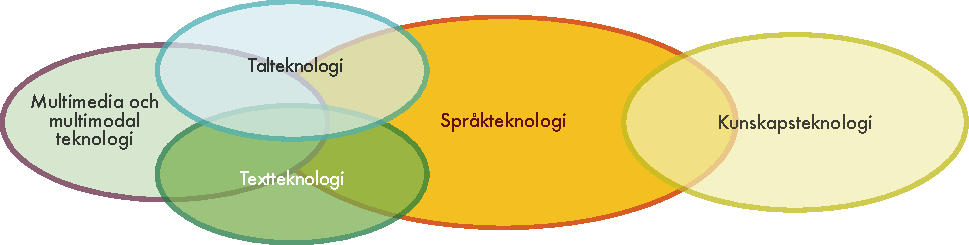
\includegraphics[width=\textwidth]{../_media/swedish/language_technologies}
  \caption{Språkteknologi}
  \label{fig:ltincontext_sv}
  \colorrule{grey3}{\textwidth}{1.5pt}
\end{figure*}

I vår kommunikation kombinerar vi språk med andra
kommunikationskanaler och informationsmedier. Talet kombineras
t.\,ex.~med gester och ansiktsuttryck. Digital text kombineras med
bilder och länkas till ljud och video. Filmer kan innehålla språk i
talad och skriven form. Med andra ord överlappar och interagerar
språkteknologi med andra teknologier för hantering och förmedling av
multimodala och multimediala data.

Nedan ska vi ge en översikt över de huvudsakliga användningsområdena
för språkteknologi, särskilt språkkontroll, webbsökteknologi, talad
interaktion och maskin\-över\-sätt\-ning. Här ingår tillämpningar och
basteknologier som exempelvis

\begin{itemize}
\item stavningskontroll
\item skrivstöd vid textproduktion
\item datorstödd språkinlärning
\item informationssökning
\item informationsextraktion
\item textsammanfattning
\item frågebesvarande system
\item taligenkänning
\item talsyntes
\end{itemize}

Språkteknologi är att väletablerat och livligt forskningsområde. För
den som är intresserad av att få veta mer om detta vittförgrenade
forskningsfält finns ett antal grundläggande och översiktliga arbeten,
t.ex.
\cite{jurafsky-martin01,manning-schuetze1,lt-world1,lt-survey1}.

Innan vi övergår till att diskutera de specifika tillämpningsområdena
närmare, ska vi beskriva hur ett typiskt språkteknologisystem är
uppbyggt.


\subsection{Tillämpnings- \ \ \ arkitekturer}

Programvara för hantering av språk består typiskt av ett antal
urskiljbara moduler, som avspeglar olika aspekter av
språket. Figur~\ref{fig:textprocessingarch_sv} visar i översiktlig och
starkt förenklad form uppbyggnaden av ett typiskt
textbearbetningssystem. De första tre modulerna svarar för att ta hand
om den inkommande textens struktur och betydelse:
\begin{enumerate}
\item förbearbetning: ``städar'' texten, analyserar eller tar bort
  formateringsinformation, samt bestämmer vilket eller vilka textens
  språk är, etc.
\item grammatisk analys: hittar verbet och dess argument (subjekt,
  objekt, etc.) och andra satsdelar, och utför en grammatisk analys av
  meningsstrukturen.
\item semantisk analys: disambiguerar flertydiga uttryck
  (d.v.s. bestämmer vilken betydelse uttrycket har i den aktuella
  kontexten), hanterar koreferens, alltså avgör vilka pronomen och
  substantiv som refererar till samma sak%i världen
, samt
  representerar språkliga uttrycks betydelse i en form som kan
  hanteras av datorprogram.
\end{enumerate}

Efter denna grundläggande textanalys kan specaliserade moduler ta sig
an specifika uppgifter, t.\,ex.~automatisk textsammanfattning eller
databassökning.

I nästa avsnitt beskriver vi översiktligt några centrala
användningsområden för språkteknologi. Därefter följer en översikt
över aktuell språkteknologiforskning och -utbildning i Sverige samt
över tidigare och nuvarande forskningsprogram. Slutligen presenterar
vi en expertuppskattning av tillgången till centrala
språkteknologiverktyg och -resurser för svenska, i termer av sådana
faktorer som tillgänglighet, mognad och kvalitet. I slutet av detta
avsnitt ges en sammanfattande lägesöversikt i en tabell
(figur~\ref{fig:lrlttable_sv} på
sidan~\pageref{fig:lrlttable_sv}). Tillämpningar och resurser som i
texten återges med fetstil återfinns även i denna tabell. Dessutom
finns i slutet av detta avsnitt en jämförelse mellan svenska och de
andra språken i vitboksserien med avseende på tillgången till
språkteknologiresurser.


\begin{figure*}[htb]
  \colorrule{grey3}{\textwidth}{1.5pt}
  \center
  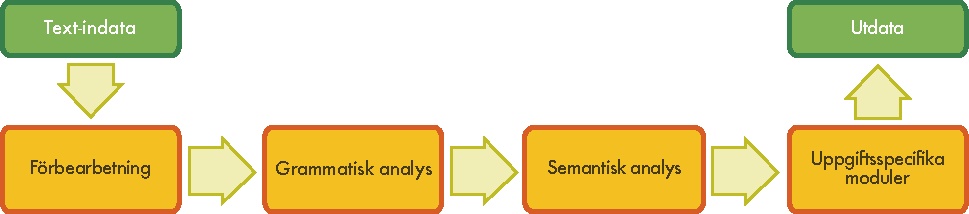
\includegraphics[width=\textwidth]{../_media/swedish/text_processing_app_architecture}
  \caption{En vanlig applikationsarkitektur för textbearbetning}
  \label{fig:textprocessingarch_sv}
  \colorrule{grey3}{\textwidth}{1.5pt}
\end{figure*}

\subsection{Centrala användningsområden} 

Här fokuserar vi på de mest centrala tillämpningarna och resurserna
samt ger en överblick över aktiviteter inom språkteknologiområdet i
Sverige.

\subsubsection{Språkgranskning}

De flesta ordbehandlingsprogram har numera en
stavningskontrollfunktion som markerar felstavningar och föreslår
korrekta alternativ. De tidigaste stavningskontrollprogrammen jämförde
en lista över orden i texten med en inbyggd lista över rättstavade
ord. Dagens språkgranskningsverktyg är mycket mer avancerade. Med
hjälp av språkspecifik \textbf{grammatisk analys} kan de upptäcka fel
både i ordböjning (t.\,ex.~felaktiga pluralformer) och i satsbyggnad,
exempelvis att verb saknas i en mening eller att fel artikel- eller
adjektivform används med ett substantiv (t.\,ex.~\textit{*en *stor
  fordon}). Däremot kommer ett språkgranskningsprogram troligen inte
att hitta några fel i följande text \cite{zar1}:

\begin{quote}
  I have a spelling checker,\\
  It came with my PC.\\
  It plane lee marks four my revue\\
  Miss steaks aye can knot sea.
\end{quote}

För att programmet ska kunna hitta denna typ av fel krävs i regel en
analys av kontexten, som i följande exempel där kontexten hjälper oss
att avgöra om det sista pronomenet i meningen ska vara ental (singular) eller
flertal (plural):

\begin{itemize}
\item \textit{Faxen} [maskin] blev tydligen \textit{skickad} [\textsc{ental}] förra veckan, men jag har inte sett \textit{den}.
\item \textit{Faxen} [meddelanden] blev tydligen \textit{skickade} [\textsc{flertal}] förra veckan, men jag har inte sett \textit{dem}.
\end{itemize}

För en analys av den här typen behövs antingen språkspecifika
\textbf{grammatiker}, formulerade och kodade för
språkteknologimjukvaran av experter -- en mycket arbetskrävande
procedur -- eller en statistisk språkmodell. I det senare fallet
beräknar modellen sannolikheten för ett visst ord i en viss position
(t.\,ex.~mellan två andra ord). Till exempel: \textit{sölig bardisk} är
en mycket sannolikare ordsekvens än \textit{sölig bar disk} (med
särskrivning av sammansättningsleden). En sådan statistisk språkmodell
kan skapas automatiskt utifrån stora mängder (korrekt) text, en
\textbf{textkorpus}. Oavsett vilken metod som används, har de flesta
tillämpningarna utvecklats för engelska, och det behöver inte med
nödvändighet vara så att de utan vidare kan användas på svensk text,
eftersom svenska uppvisar större frihet i ordföljden och använder en
stor mängd sammansättningar.


\begin{figure*}[htb]
  \colorrule{grey3}{\textwidth}{1.5pt}
  \center
  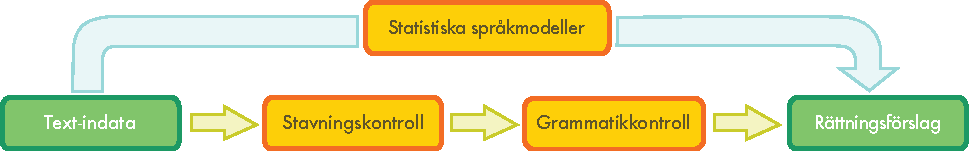
\includegraphics[width=\textwidth]{../_media/swedish/language_checking}
  \caption{Språkkontroll (överst: statistisk, underst: regelbaserad)}
  \label{fig:langcheckingaarch_sv}
  \colorrule{grey3}{\textwidth}{1.5pt}
\end{figure*}

Språkgranskning används inte bara i
ordbehandlingsprogram. Språkgranskningsverktyg återfinns även
integrerade i form av skrivstödsfunktioner i system för
dokumentproduktion, d.v.s. system avsedda för produktion av
standardiserade manualer och annan dokumentation för exempelvis
komplexa produkter och system inom IT, vård och industri. I syfte att
undvika kundklagomål om användningssvårigheter och skadeståndskrav som
ytterst beror på svårbegripliga instruktioner, fokuserar företag i
ökande grad på kvaliteten i sin dokumentation, samtidigt som de i
ökande grad riktar sig till en internationell marknad (med åtföljande
översättning och lokalisering av produkter och
dokumentation). Språkteknologiska komponenter i systemen för
dokumentproduktion hjälper därvid de tekniska skribenterna att använda
det ordförråd och den meningsbyggnad och övriga språkliga strukturer
som föreskrivs i företags- och branchspecifika skrivregelsamlingar.

\boxtext{Språkgranskning -- från ordbehandling till generellt skrivstöd.}

Det finns ett litet antal svenska företag som använder eller erbjuder
produkter och tjänster av detta slag, däribland Scania och några
mindre språkteknologiföretag.

Språkgranskning används dock inte enbart i
stav\-nings\-kon\-troll\-pro\-gram och system för
dokumentproduktion. Den förekommer även i datorstödd språkinlärning
och för att föreslå alternativa (korrigerade) sökord i sökmotorer, som
Googles \textit{Menade du~\ldots}-förslag.

Oribi (\url{http://www.oribi.se}) är ett svenskt småföretag som
utvecklar datorstöd -- bl.a. stavningskontroll och ordprediktion --
för personer med läs- och skrivsvårigheter.

\subsubsection{Sökning på webben}

Sökning på webben, i intranät eller i digitala bib\-lio\-tek är
förmodligen den mest spridda tillämp\-ning\-en av språkteknologi idag,
samtidigt som den paradoxalt nog är relativt underutvecklad i det
avseendet. Googles sökmotor, som introducerades 1998, svarar idag för
ungefär 80~\% av alla sökningar på webben \cite{spi1}. Verbet
\textit{googla} återfinns redan i svenska ordböcker (t.\,ex.~i senaste
upplagan av SAOL). Googles sökgränssnitt och träffsida har inte
förändrats i grunden sen den första versionen. Däremot har man infört
både stavningskorrigering och en rudimentär semantisk sökning som
bygger på en kontextuell analys av sökorden i relation till andra ord
i sökfrågan \cite{pc1}. Googles framgångar visar hur tillgång till
stora datamängder i kombination med effektiva
in\-dex\-er\-ings\-tek\-nik\-er och statistiskt baserad språkteknologi
kan producera godtagbara resultat för denna typ av sökningar på
webben.

\begin{figure*}[htb]
  \colorrule{grey3}{\textwidth}{1.5pt}
  \center
  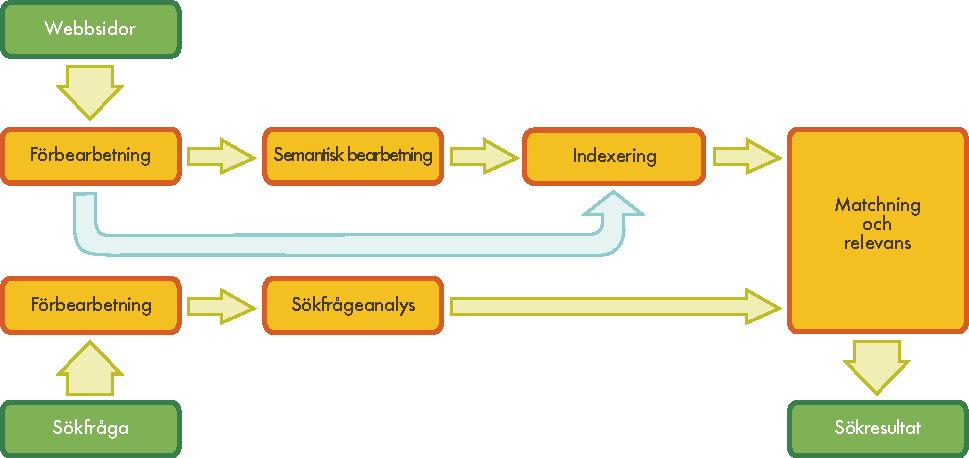
\includegraphics[width=\textwidth]{../_media/swedish/web_search_architecture}
  \caption{Webbsökning}
  \label{fig:websearcharch_sv}
  \colorrule{grey3}{\textwidth}{1.5pt}
\end{figure*}

När informationsbehoven växer i komplexitet blir det dock viktigt att
kunna bygga in mer språkkunskap i systemen för att kunna tolka
sökfrågorna och texten i de dokument som söks fram. Här har man
experimenterat med att använda den semantiska informationen i
\textbf{lexikonresurser} (t.\,ex.~maskinläsbara begreppsordböcker --
tesaurusar -- som WordNet för engelska eller SALDO för
svenska\cite{saldo1}) och därvid
lyckats förbättra sökresultaten genom att använda synonymer till de
ursprungliga sökorden, t.\,ex.~\textit{atomkraft}, \textit{kärnkraft}
and \textit{kärnenergi}, eller rentav bara mer löst relaterade ord
(som \textit{fission} eller \textit{reaktor}).

\boxtext{Nästa sökmotorgeneration behöver mycket mer sofistikerad språkteknologi.}

Nästa generation av sökmotorer måste använda mycket mer sofistikerad
språkteknologi, särskilt för att hantera sökfrågor formulerade som
riktiga frågor eller uppmaningar snarare än som en mängd sökord. För
en sökfråga som \textit{Ge mig en förteckning över alla företag som
  har köpts upp av andra företag under de senaste fem åren}, krävs
både en syntaktisk och en \textbf{semantisk analys}. Ett söksystem 
måste även indexera dokumentsamlingen för att snabbt hitta de
relevanta dokumenten. För att komma fram till ett svar på frågan
behöver sökmotorn analysera dess grammatiska struktur för att förstå
att vad som efterfrågas är de företag som har blivit uppköpta och inte
de företag som stått för uppköpen. För att kunna tolka uttrycket
\textit{de senaste fem åren} måste systemet bestämma vilket
tidsintervall det handlar om och förstå att innevarande år ska räknas
med i det. Frågan ska sedan matchas mot en mycket stor mängd texter
för att finna informationsfragment som tillsammans kan användas för
att sätta ihop ett svar. Matchnings\-pro\-cess\-en kallas
informationssökning och inbegriper bland annat metoder för att söka
igenom dokumentsam\-ling\-en och rangordna sökträffarna. För att
sammanställa den efterfrågade förteckningen över företag, måste
systemet känna igen de ordföljder i dokumenten som utgör företagsnamn
genom en process som brukar kallas namnigenkänning.

En ännu större utmaning består i att matcha en sökfråga på ett språk
med dokument på ett annat språk. Tvärspråklig informationssökning
innefattar översättning av sökfrågan till alla språk som förekommer i
dokumentsamlingen samt översättning av de funna dokumenten till
användarens språk. Utvecklingen går snabbt därhän att alltmer information på webben är
multimedial, vilket skapar ett behov av motsvarande sökfunktioner
direkt i bild-, ljud- och vi\-deo\-data. I ljud- och vi\-deo\-data måste en
taligenkänningsmodul användas för att omvandla talat språk till text,
som sedan kan matchas mot en sökfråga. Både allmänna teknologier med öppen källkod som Lucene och SOLr och
internationella söklösningar som FAST och Exalead används flitigt av
företag som grundkomponenter i specialiserade sök\-lös\-ning\-ar. Utvecklingen fokuserar i sådana företag på att tillhandahålla
tilläggsmoduler och avancerade sökmotorer för webbportaler genom att
utnyttja ämnesspecifik semantisk information. Eftersom detta innebär
mycket resurskrävande bearbetningar, är sådana sökmotorer ekonomiskt
realistiska endast med relativt små textkorpusar. Bearbetningstiden
kan lätt bli flera storleksordningar större än för en statistiskt
baserad sökmotor som Google. Detta tillsammans med behovet av relativt
omfattande ämnesspecifik domänmodellering gör att denna teknologi för
närvarande inte skalar upp för användning på webben som helhet.

I Sverige gjorde Hapax (\url{http://www.hapax.com}; nu Open\-Amplify) en
stor satsning på att utveckla denna typ av teknologi under åren
2000--2005. Ett företag som använder språkteknologi i fler\-språkiga
sök\-lösningar framför allt för företags\-intra\-nät är Findwise
(\url{http://www.findwise.com}). Ett relativt nystartat svenskt
företag är Gavagai (\url{http://www.gavagai.se}).


\subsubsection{Talad interaktion}

\begin{figure*}[htb]
  \colorrule{grey3}{\textwidth}{1.5pt}
  \center 
  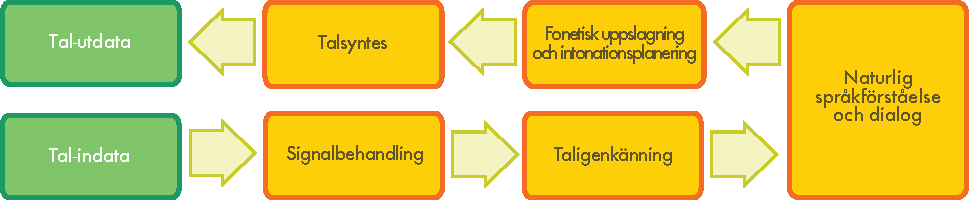
\includegraphics[width=\textwidth]{../_media/swedish/simple_speech-based_dialogue_architecture}
  \caption{Talbaserad dialogarkitektur}
  \label{fig:dialoguearch_sv}
  \colorrule{grey3}{\textwidth}{1.5pt}
\end{figure*}

Talad interaktion -- dialoger mellan människor och datorsystem av
olika slag -- är ett tillämpningsområde för talteknologi, alltså att
få datorer att förstå och producera talat språk. Talteknologi används
för att utveckla gränssnitt som låter användarna tala med
tillämpningarna istället för att använda bildskärm, tangentbord och
mus för interaktionen. Idag återfinner vi sådana talgränssnitt eller
dialogsystem i delvis eller helt automatiserade talsvarstjänster,
framför allt hos företag inom \mbox{bank-,} leverantörs-, transport-
och telekommunikationssektorerna. Talgränssnitt förekommer även
exempelvis i GPS-system i bilar samt som ett alternativ till
pek\-skärm\-en i smarttelefoner. Talgränssnitt eller dialogsystem omfattar följande fyra
forskningsområden:

\begin{enumerate}
\item Automatisk \textbf{taligenkänning} (\emph{Automatic Speech
  Recognition: ASR}) omvandlar den ljudföljd som användaren yttrar
  till den mest sannolika ordsekvensen med hjälp av en statistisk
  modell.
\item Språkanalys bestämmer yttrandets grammatiska struktur samt
  tolkar användarens yttrande i relation till det aktuella systemet,
  med hjälp av regler och/eller statistik.
\item Dialoghantering avgör på grundval av det analyserade yttrandet
  och dialoghistorik vilken systemfunktion som ska aktiveras.
\item \textbf{Talsyntes} (text-till-tal; \emph{Text-to-Speech: TTS})
  genererar en talad version av systemets svar.
\end{enumerate}

En av de största utmaningarna för tal\-igen\-känn\-ings\-sys\-tem är att med
godtagbar noggrannhet avgöra vilka ord en användare har yttrat. Det
kan göras genom att begränsa tillåtna yttranden till en liten mängd
nyckelord eller genom att manuellt skapa språkmodeller som täcker en
stor mängd yttranden och talare. Med maskininlärningstekniker kan
sådana språkmodeller ävan skapas automatiskt från taladatabaser eller
\textbf{talkorpusar}, d.v.s. stora samlingar transkriberade
taldata. Om man begränsar mängden yttranden som ett
taligenkänningssystem kan hantera, leder detta inte sällan till att
interaktionen uppfattas som styltad vilket kan påverka acceptansen för
gränssnittet negativt. Å andra sidan är det förknippat med betydande
kostnader att skapa, anpassa och underhålla omfattande
språkmodeller. Dialogsystem som inkluderar språkmodeller (normalt
automatiskt skapade från talkorpusar) och som tillåter användarna att
uttrycka sina önskemål på ett mer varierat sätt -- t.\,ex.~genom att
inleda dialogen med \textit{Hur kan jag stå till tjänst?} -- tenderar
att accepteras bättre av användarna.

\boxtext{Talteknologi används för att utveckla gränssnitt som låter
  användarna tala med tillämpningarna istället för att använda
  bildskärm, tangentbord och mus för interaktionen.}

I kommersiella system används ofta yttranden inlästa av professionella
inläsare för att generera talgränssnittets svar. Om svaret inte ska
innehålla någon del som är beroende av den specifika kontexten eller
av användardata, utan ett inspelat yttrande kan återanvändas i sin
helhet, kan en rik användarupplevelse uppnås. Om svaret däremot ska
anpassas i något avseende, kan resultatet bli undermåligt om detta för
med sig att systemet behöver klippa och klistra ihop bitar av de olika
inspelade yttranden, något som kan leda till att resultatet får en
onaturlig satsmelodi. Även om talsyntessystemen blir allt bättre på
att på detta sätt generera yttranden som låter naturliga, finns det
fortfarande mycket utrymme för förbättring inom detta område.

De komponenter som ingår i ett typiskt talgränssnitt på dagens marknad
har genomgått en långt driven standardisering under det senaste
årtiondet. Marknaden för taligenkänning och talsyntes har också
konsoliderats starkt under samma tid. I G20-länderna (starka ekonomier
med stor befolkning) har de nationella marknaderna dominerats av fem
globala företag, med Nuance (USA) och Loquendo (Italien) som de mest
framträdande. En ytterligare konsolidering av marknaden skedde 2011,
då Nuance köpte upp Loquendo.

På den svenska marknaden finns talsyntesröster för svenska utvecklade
av bl.a. Stockholmsföretaget Acapela och det statliga Talboks- och
punktskriftsbiblioteket (TPB). Det finns också en stark svensk
tal\-tekno\-logi\-forsk\-ning, med centrum vid KTH i Stockholm (som
har utvecklat ett antal egna system).

Marknaden för dialoghanteringsteknologi domineras starkt av
nationella, ofta små företag. De viktigaste aktörerna på den svenska
marknaden är idag Artificial Solutions och SpeechCraft. Bland mindre
företag på den svenska marknaden kan nämnas
Talkamatic (\url{http://www.talkamatic.se/}), som utvecklar
dialogsystem åt fordonsindustrin för användning i bilar. Dessa företag
bygger inte i första hand på utlicensiering av sin mjukvara, utan de
levererar hela talgränssnitt för integrering i specifika
systemmiljöer. Slutligen kan nämnas att det ännu inte har uppstått
någon riktig marknad för de grammatiska och semantiska
analysteknologierna i dialogsystem.

När det gäller faktisk användning av talgränssnitt har efterfrågan
ökat drastiskt i Sverige under de senaste 10 åren. Detta har framför
allt betingats av slutkundernas ökade krav på
själv\-be\-tjän\-ings\-möj\-lig\-het\-er, av den avsevärda
kost\-nads\-opti\-mer\-ings\-poten\-tial\-en i talsvarstjänster, samt
ökad acceptans för tal som medium för människa-datorinteraktion. En
viktig katalysator har också varit inrättandet av den svenska
nationella forskarskolan i språkteknologi (\emph{Graduate School of
  Language Technology: GSLT}) och därmed uppkomsten av ett livaktigt
nationellt nätverk av språkteknologiforskare, industriaktörer och
företagskunder. GSLT har i samarbete med andra organiserat nationella
work\-shop\-ar och inbjudit industrirepresentanter att hålla seminarier
för de forskarstuderande. De akademiska forskningsmiljöerna CLT
(\emph{Centre for Language Technology}) i Göteborg och Institutionen
för tal, musik och hörsel vid KTH i Stockholm har deltagit aktivt i
dessa aktiviteter för att sprida kunskap om talgränssnitts- och
dialogteknologier bland svenska företag.

Vi ser nu en utveckling där smarttelefoner håller på att etablera sig
som en ny viktig plattform för kundrelationer, i tillägg till fast
telefoni, internet och epost. Detta kommer också att påverka
användningen av talteknologi. På längre sikt kommer vi att se fler
talsvarssystem på fler områden, och talbaserade appar kommer att spela
en betydligt större roll som användarvänliga gränssnitt i
smarttelefoner. Denna utveckling kommer att drivas på av den ständiga
förbättring av talaroberoende taligenkänning som möjliggörs genom de
stora mängder taldata som ackumuleras i de centraliserade
dikteringstjänster som redan är tillgängliga för smattelefonanvändare.


\subsubsection{Maskin\-över\-sätt\-ning}

Idén att datorer skulle kunna översätta automatiskt mellan olika språk
lanserades redan i datorernas barndom 1946. Under 1950-talet och
återigen under 1980-talet har betydande summor satsats på forskning i
\textbf{maskin\-över\-sätt\-ning}, men trots det kan datorer fortfarande
inte uppfylla det gamla löftet om generell automatisk översättning.

\boxtext{Den enklaste maskin\-över\-sätt\-ningsmetoden är helt enkelt att
  byta ut varje källspråksord mot motsvarande målspråksord.}

Den enklaste metoden för maskin\-över\-sätt\-ning är helt enkelt att orden i
källspråkstexten byts ut mot motsvarande ord i målspråket. Detta kan
fungera i mycket begränsade domäner med formelartat språk, som
t.\,ex.~väderleksrapporter. Vill man prestera översättningar av god
kvalitet av mindre begränsade texter är det nödvändigt att passa ihop
större språkliga enheter (fraser, meningar eller ibland även längre
textavsnitt) med deras närmaste motsvarigheter i målspråket. Den
största stötestenen är att våra språk är fulla av flertydigheter,
vilket leder till komplikationer på alla språkliga nivåer. Det kan
handla om enstaka ord -- här talar man om lexikal disambiguering (en
\textit{jaguar} kan vara en bil eller ett djur) -- eller om
frågan om vilken roll ett prepositionsuttryck spelar i satsen,
attribut eller adverbial, till exempel:

\begin{itemize}
\item \textit{Polisen betraktade mannen med kikaren.}
\item \textit{Polisen betraktade mannen med revolvern.}
\end{itemize}

\begin{figure*}[htb]
  \colorrule{grey3}{\textwidth}{1.5pt}
  \center
  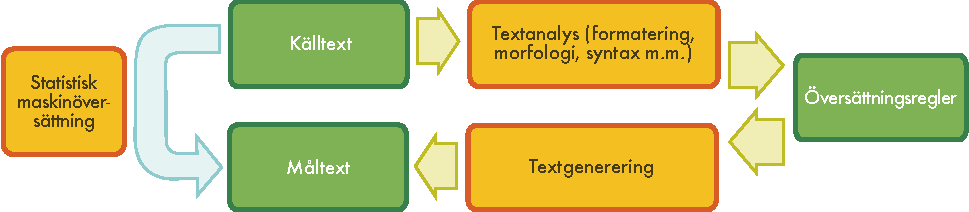
\includegraphics[width=\textwidth]{../_media/swedish/machine_translation}
  \caption{Maskinöversättning (till vänster: statistisk, till höger: regelbaserad)}
  \label{fig:mtarch_sv}
  \colorrule{grey3}{\textwidth}{1.5pt}
\end{figure*}

Ett maskin\-över\-sätt\-nings\-system kan byggas med hjälp av språkliga regler
(en grammatik). För översättning mellan närbesläktade språk kan en
ord-för-ord- eller fras-för-fras-översättning som den som skisserades
ovan fungera väl. Regelbaserade maskin\-över\-sätt\-nings\-system fungerar
dock normalt så att de analyserar källspråkstexten och skapar en
mellanliggande symbolisk representation som sen kan ligga till grund
för generering av målspråkstexten. Hur bra ett regelbaserat system
fungerar är ytterst beroende på tillgänglighet och kvalitet hos stora
lexikonresurser med morfologisk, syntaktisk och semantisk information,
samt omfattande uppsättningar av grammatikregler (för både analys och
generering) noggrant formulerade av språkvetare. Detta är en
omfattande och därmed mycket kostsam arbetsinsats.

Mot slutet av 1980-talet, när datorerna snabbt blev snabbare och
billigare, började intresset växa för tillämpningen av statistiska
modeller i maskin\-över\-sätt\-ning. Dessa är resultatet av analys av
tvåspråkiga textkorpusar, \textbf{parallellkorpusar}, exempelvis
Europarlkorpusen, som innehåller Europaparlamentets protokoll på 21
EU-språk. Med tillräckligt stora data\-mängd\-er till sitt förfogande
kan statistisk maskin\-över\-sätt\-ning ge ett godtagbart resultat. Man får
en unge\-fär\-lig version av källspråkets text som är resultatet av
statistisk analys av parallella texter och identifiering av troliga
ord\-mönster\-mot\-svarig\-het\-er. I motsats till kunskapsbaserade
system producerar dock statistisk (eller datadriven)
maskin\-över\-sätt\-ning ofta icke-välformat (ogrammatiskt)
språk. Datadriven maskin\-över\-sätt\-ning har den fördelen att den kräver
betydligt mindre manuell arbetsinsats och den kan också uppvisa bättre
täckning av vissa specifika språkfenomen -- exempelvis idiomatiska
uttryck -- som ofta behandlas styvmoderligt i kunskapsbaserade system.

Kunskapsbaserade och datadrivna maskin\-över\-sätt\-ningssystem tenderar att
uppvisa komplementära styrkor och brister. Därför fokuserar dagens
forskning inom området på att utveckla hybridsystem där de två
metoderna kombineras, t.\,ex.~genom att låta ett system av varje slag
översätta samma text och tillföra en ur\-vals\-algo\-ritm som för
varje översatt mening väljer den bästa översättningen enligt något
formaliserbart kriterium. Det visar sig dock att för längre meningar
(t.\,ex.~mer än 12 ord långa) blir resultatet ofta undermåligt oavsett
vilket system det gäller. En mer effektiv lösning är istället att
kombinera ihop de bästa delarna från samma mening översatt med två
eller flera olika system, en procedur som kan bli mycket komplex,
eftersom det inte alltid är uppenbart vilka delar som motsvarar
varandra, utan man behöver ta till samma typ av metoder som används
för att hitta översättningsmotsvarigheter i parallelltexter.

Svenskan erbjuder flera utmaningar för maskin\-över\-sätt\-ning. I
ordbildningssystemet leder möjligheten att fritt bilda nya tillfälliga
sammansättningar till svårigheter för den lexikala analysen. I
grammatiken gör den friare ordföljden det svårare att identifiera
satsens huvudled och växlingen i partikelverb mellan fristående
partiklar i vissa former och bundna prefix i andra komplicerar den
lexikala analysen.

För närvarande ingår svenska i språkutbudet för ett litet antal
maskin\-över\-sätt\-ningssystem och bara några av de större kommersiella
aktörerna på marknaden arbetar aktivt med utveckling av
maskin\-över\-sätt\-ning till och från svenska. Det finns även några mindre
företag på området, t.\,ex.~Convertus AB (\url{http://www.convertus.se}).

\boxtext{Svenskan erbjuder flera utmaningar för maskinöversättning.} 

Maskin\-över\-sätt\-ning kan öka produktiviteten avsevärt under
förutsättning att systemen kan an\-pas\-sas med avseende på
terminologi och integrering i arbetsflödet. Kommersiella aktörer har
utvecklat specialsystem för interaktivt
översättningsstöd. Språkportaler ger tillgång till allmänna
lexikonresurser och företagsspecifika terminologiresurser,
översättningsminnen och maskin\-över\-sätt\-ningsfunktioner. Ett svenskt
småföretag som specialicerat sig på flerspråkig terminologiutvinning
och terminologihantering är Fodina Language
Technology (\url{http://www.fodina.se}).

Förbättringspotentialen för maskin\-över\-sätt\-nings\-sys\-tem är fortfarande
enorm. Bland utmaningarna kan nämnas anpassning av språkresurser till
en viss domän eller ett visst användningsområde, samt integrering av
teknologin i arbetsflöden där man redan använder sig av termbaser och
översättningsminnen. Ett annat problem är att de flesta systemen är
inriktade på engelska och stöder på sin höjd översättning av något
enstaka språk till och från svenska direkt. Detta leder till
ineffektivitet i översättningsarbetet eftersom flera olika system
behöver användas parallellt (beroende på det aktuella språkparet) med
olika verktyg och konventioner för exempelvis tillägg av lexikal
information.

Utvärderingskampanjer underlättar kvalitetsjämförelser mellan
maskin\-över\-sätt\-ningssystem och maskin\-över\-sätt\-ningsmetoder samt
jämförelser mellan status för olika språkpar. I
figur~\ref{fig:euromatrix_sv} från EU-projektet EuroMatrix+ ser vi
resultaten av maskin\-över\-sätt\-ning mellan alla par av 22 av de 23
officiella EU-språken (iriska var inte med i jämförelsen). Resultaten
ges i form av BLEU-poäng \cite{bleu1}. BLEU är en helautomatisk
utvärderingsmetod för maskin\-över\-sätt\-ning som ger en grov uppskattning
av kvaliteten hos en översättning. Bättre översättningar får högre
poäng, och en mänsklig översättare borde normalt hamna på ungefär 80
BLEU-poäng.

De bästa siffrorna (gröna och blå) finner vi för språk där man har
lagt ner betydande forskningsinsatser i samordnade forskningsprogram
och där man dessutom förfogar över många och stora parallellkorpusar
(t.\,ex.~engelska, franska, nederländska, spanska och tyska). De språk
som uppvisar sämre resultat (återgivna med röda siffror) är sådana där
antingen utvecklingsinsatserna saknas delvis eller helt, eller där
språken i strukturellt hänseende skiljer sig starkt från de övriga
(t.\,ex.~ungerska, maltesiska och finska).


\begin{figure*}[htbp]
  \centering
  \setlength{\tabcolsep}{0.17em}
  \small
  \begin{tabular}{>{\columncolor{corange1}}cccccccccccccccccccccccc}
%    & \multicolumn{22}{>{\columncolor{corange1}}c}{Målspråk -- \textcolor{grey1}{Target language}}\\\addlinespace[{-.009cm}]
    & \multicolumn{22}{>{\columncolor{corange1}}c}{Målspråk -- \textcolor{grey1}{Target language}}\\\addlinespace[{-.009cm}]
    \rowcolor{corange1}  & EN & BG & DE & CS & DA & EL & ES & ET & FI & FR & HU & IT & LT & LV & MT & NL & PL & PT & RO & SK & SL & SV\\
    EN & -- & \textcolor{blue}{40,5} & \textcolor{blue}{46,8} & \textcolor{green2}{52,6} & \textcolor{green2}{50,0} & \textcolor{blue}{41,0} & \textcolor{green2}{55,2} & \textcolor{purple}{34,8} & \textcolor{purple}{38,6} & \textcolor{green2}{50,1} & \textcolor{purple}{37,2} & \textcolor{green2}{50,4} & \textcolor{purple}{39,6} & \textcolor{blue}{43,4} & \textcolor{purple}{39,8} & \textcolor{green2}{52,3} & \textcolor{blue}{49,2} & \textcolor{green2}{55,0} & \textcolor{blue}{49,0} & \textcolor{blue}{44,7} & \textcolor{green2}{50,7} & \textcolor{green2}{52,0}\\
    BG & \textcolor{green}{61,3} & -- & \textcolor{purple}{38,7} & \textcolor{purple}{39,4} & \textcolor{purple}{39,6} & \textcolor{purple}{34,5} & \textcolor{blue}{46,9} & \textcolor{red3}{25,5} & \textcolor{red3}{26,7} & \textcolor{blue}{42,4} & \textcolor{red3}{22,0} & \textcolor{blue}{43,5} & \textcolor{red3}{29,3} & \textcolor{red3}{29,1} & \textcolor{red3}{25,9} & \textcolor{blue}{44,9} & \textcolor{purple}{35,1} & \textcolor{blue}{45,9} & \textcolor{purple}{36,8} & \textcolor{purple}{34,1} & \textcolor{purple}{34,1} & \textcolor{purple}{39,9}\\
    DE & \textcolor{green2}{53,6} & \textcolor{red3}{26,3} & -- & \textcolor{purple}{35,4} & \textcolor{blue}{43,1} & \textcolor{purple}{32,8} & \textcolor{blue}{47,1} & \textcolor{red3}{26,7} & \textcolor{red3}{29,5} & \textcolor{purple}{39,4} & \textcolor{red3}{27,6} & \textcolor{blue}{42,7} & \textcolor{red3}{27,6} & \textcolor{purple}{30,3} & \textcolor{red2}{19,8} & \textcolor{green2}{50,2} & \textcolor{purple}{30,2} & \textcolor{blue}{44,1} & \textcolor{purple}{30,7} & \textcolor{red3}{29,4} & \textcolor{purple}{31,4} & \textcolor{blue}{41,2}\\
    CS & \textcolor{green2}{58,4} & \textcolor{purple}{32,0} & \textcolor{blue}{42,6} & -- & \textcolor{blue}{43,6} & \textcolor{purple}{34,6} & \textcolor{blue}{48,9} & \textcolor{purple}{30,7} & \textcolor{purple}{30,5} & \textcolor{blue}{41,6} & \textcolor{red3}{27,4} & \textcolor{blue}{44,3} & \textcolor{purple}{34,5} & \textcolor{purple}{35,8} & \textcolor{red3}{26,3} & \textcolor{blue}{46,5} & \textcolor{purple}{39,2} & \textcolor{blue}{45,7} & \textcolor{purple}{36,5} & \textcolor{blue}{43,6} & \textcolor{blue}{41,3} & \textcolor{blue}{42,9}\\
    DA & \textcolor{green2}{57,6} & \textcolor{red3}{28,7} & \textcolor{blue}{44,1} & \textcolor{purple}{35,7} & -- & \textcolor{purple}{34,3} & \textcolor{blue}{47,5} & \textcolor{red3}{27,8} & \textcolor{purple}{31,6} & \textcolor{blue}{41,3} & \textcolor{red3}{24,2} & \textcolor{blue}{43,8} & \textcolor{red3}{29,7} & \textcolor{purple}{32,9} & \textcolor{red3}{21,1} & \textcolor{blue}{48,5} & \textcolor{purple}{34,3} & \textcolor{blue}{45,4} & \textcolor{purple}{33,9} & \textcolor{purple}{33,0} & \textcolor{purple}{36,2} & \textcolor{blue}{47,2}\\
    EL & \textcolor{green2}{59,5} & \textcolor{purple}{32,4} & \textcolor{blue}{43,1} & \textcolor{purple}{37,7} & \textcolor{blue}{44,5} & -- & \textcolor{green2}{54,0} & \textcolor{red3}{26,5} & \textcolor{red3}{29,0} & \textcolor{blue}{48,3} & \textcolor{red3}{23,7} & \textcolor{blue}{49,6} & \textcolor{red3}{29,0} & \textcolor{purple}{32,6} & \textcolor{red3}{23,8} & \textcolor{blue}{48,9} & \textcolor{purple}{34,2} & \textcolor{green2}{52,5} & \textcolor{purple}{37,2} & \textcolor{purple}{33,1} & \textcolor{purple}{36,3} & \textcolor{blue}{43,3}\\
    ES & \textcolor{green}{60,0} & \textcolor{purple}{31,1} & \textcolor{blue}{42,7} & \textcolor{purple}{37,5} & \textcolor{blue}{44,4} & \textcolor{purple}{39,4} & -- & \textcolor{red3}{25,4} & \textcolor{red3}{28,5} & \textcolor{green2}{51,3} & \textcolor{red3}{24,0} & \textcolor{green2}{51,7} & \textcolor{red3}{26,8} & \textcolor{purple}{30,5} & \textcolor{red3}{24,6} & \textcolor{blue}{48,8} & \textcolor{purple}{33,9} & \textcolor{green2}{57,3} & \textcolor{purple}{38,1} & \textcolor{purple}{31,7} & \textcolor{purple}{33,9} & \textcolor{blue}{43,7}\\
    ET & \textcolor{green2}{52,0} & \textcolor{red3}{24,6} & \textcolor{purple}{37,3} & \textcolor{purple}{35,2} & \textcolor{purple}{37,8} & \textcolor{red3}{28,2} & \textcolor{blue}{40,4} & -- & \textcolor{purple}{37,7} & \textcolor{purple}{33,4} & \textcolor{purple}{30,9} & \textcolor{purple}{37,0} & \textcolor{purple}{35,0} & \textcolor{purple}{36,9} & \textcolor{red3}{20,5} & \textcolor{blue}{41,3} & \textcolor{purple}{32,0} & \textcolor{purple}{37,8} & \textcolor{red3}{28,0} & \textcolor{purple}{30,6} & \textcolor{purple}{32,9} & \textcolor{purple}{37,3}\\
    FI & \textcolor{blue}{49,3} & \textcolor{red3}{23,2} & \textcolor{purple}{36,0} & \textcolor{purple}{32,0} & \textcolor{purple}{37,9} & \textcolor{red3}{27,2} & \textcolor{purple}{39,7} & \textcolor{purple}{34,9} & -- & \textcolor{red3}{29,5} & \textcolor{red3}{27,2} & \textcolor{purple}{36,6} & \textcolor{purple}{30,5} & \textcolor{purple}{32,5} & \textcolor{red2}{19,4} & \textcolor{blue}{40,6} & \textcolor{red3}{28,8} & \textcolor{purple}{37,5} & \textcolor{red3}{26,5} & \textcolor{red3}{27,3} & \textcolor{red3}{28,2} & \textcolor{purple}{37,6}\\
    FR & \textcolor{green}{64,0} & \textcolor{purple}{34,5} & \textcolor{blue}{45,1} & \textcolor{purple}{39,5} & \textcolor{blue}{47,4} & \textcolor{blue}{42,8} & \textcolor{green}{60,9} & \textcolor{red3}{26,7} & \textcolor{purple}{30,0} & -- & \textcolor{red3}{25,5} & \textcolor{green2}{56,1} & \textcolor{red3}{28,3} & \textcolor{purple}{31,9} & \textcolor{red3}{25,3} & \textcolor{green2}{51,6} & \textcolor{purple}{35,7} & \textcolor{green}{61,0} & \textcolor{blue}{43,8} & \textcolor{purple}{33,1} & \textcolor{purple}{35,6} & \textcolor{blue}{45,8}\\
    HU & \textcolor{blue}{48,0} & \textcolor{red3}{24,7} & \textcolor{purple}{34,3} & \textcolor{purple}{30,0} & \textcolor{purple}{33,0} & \textcolor{red3}{25,5} & \textcolor{purple}{34,1} & \textcolor{red3}{29,6} & \textcolor{red3}{29,4} & \textcolor{purple}{30,7} & -- & \textcolor{purple}{33,5} & \textcolor{red3}{29,6} & \textcolor{purple}{31,9} & \textcolor{red2}{18,1} & \textcolor{purple}{36,1} & \textcolor{red3}{29,8} & \textcolor{purple}{34,2} & \textcolor{red3}{25,7} & \textcolor{red3}{25,6} & \textcolor{red3}{28,2} & \textcolor{purple}{30,5}\\
    IT & \textcolor{green}{61,0} & \textcolor{purple}{32,1} & \textcolor{blue}{44,3} & \textcolor{purple}{38,9} & \textcolor{blue}{45,8} & \textcolor{blue}{40,6} & \textcolor{red3}{26,9} & \textcolor{red3}{25,0} & \textcolor{red3}{29,7} & \textcolor{green2}{52,7} & \textcolor{red3}{24,2} & -- & \textcolor{red3}{29,4} & \textcolor{purple}{32,6} & \textcolor{red3}{24,6} & \textcolor{green2}{50,5} & \textcolor{purple}{35,2} & \textcolor{green2}{56,5} & \textcolor{purple}{39,3} & \textcolor{purple}{32,5} & \textcolor{purple}{34,7} & \textcolor{blue}{44,3}\\
    LT & \textcolor{green2}{51,8} & \textcolor{red3}{27,6} & \textcolor{purple}{33,9} & \textcolor{purple}{37,0} & \textcolor{purple}{36,8} & \textcolor{red3}{26,5} & \textcolor{red3}{21,1} & \textcolor{purple}{34,2} & \textcolor{purple}{32,0} & \textcolor{purple}{34,4} & \textcolor{red3}{28,5} & \textcolor{purple}{36,8} & -- & \textcolor{blue}{40,1} & \textcolor{red3}{22,2} & \textcolor{purple}{38,1} & \textcolor{purple}{31,6} & \textcolor{purple}{31,6} & \textcolor{red3}{29,3} & \textcolor{purple}{31,8} & \textcolor{purple}{35,3} & \textcolor{purple}{35,3}\\
    LV & \textcolor{green2}{54,0} & \textcolor{red3}{29,1} & \textcolor{purple}{35,0} & \textcolor{purple}{37,8} & \textcolor{purple}{38,5} & \textcolor{red3}{29,7} & \textcolor{red2}{8,0} & \textcolor{purple}{34,2} & \textcolor{purple}{32,4} & \textcolor{purple}{35,6} & \textcolor{red3}{29,3} & \textcolor{purple}{38,9} & \textcolor{purple}{38,4} & -- & \textcolor{red3}{23,3} & \textcolor{blue}{41,5} & \textcolor{purple}{34,4} & \textcolor{purple}{39,6} & \textcolor{purple}{31,0} & \textcolor{purple}{33,3} & \textcolor{purple}{37,1} & \textcolor{purple}{38,0}\\
    MT & \textcolor{green}{72,1} & \textcolor{purple}{32,2} & \textcolor{purple}{37,2} & \textcolor{purple}{37,9} & \textcolor{purple}{38,9} & \textcolor{purple}{33,7} & \textcolor{blue}{48,7} & \textcolor{red3}{26,9} & \textcolor{red3}{25,8} & \textcolor{blue}{42,4} & \textcolor{red3}{22,4} & \textcolor{blue}{43,7} & \textcolor{purple}{30,2} & \textcolor{purple}{33,2} & -- & \textcolor{blue}{44,0} & \textcolor{purple}{37,1} & \textcolor{blue}{45,9} & \textcolor{purple}{38,9} & \textcolor{purple}{35,8} & \textcolor{blue}{40,0} & \textcolor{blue}{41,6}\\
    NL & \textcolor{green2}{56,9} & \textcolor{red3}{29,3} & \textcolor{blue}{46,9} & \textcolor{purple}{37,0} & \textcolor{blue}{45,4} & \textcolor{purple}{35,3} & \textcolor{blue}{49,7} & \textcolor{red3}{27,5} & \textcolor{red3}{29,8} & \textcolor{blue}{43,4} & \textcolor{red3}{25,3} & \textcolor{blue}{44,5} & \textcolor{red3}{28,6} & \textcolor{purple}{31,7} & \textcolor{red3}{22,0} & -- & \textcolor{purple}{32,0} & \textcolor{blue}{47,7} & \textcolor{purple}{33,0} & \textcolor{purple}{30,1} & \textcolor{purple}{34,6} & \textcolor{blue}{43,6}\\
    PL & \textcolor{green}{60,8} & \textcolor{purple}{31,5} & \textcolor{blue}{40,2} & \textcolor{blue}{44,2} & \textcolor{blue}{42,1} & \textcolor{purple}{34,2} & \textcolor{blue}{46,2} & \textcolor{red3}{29,2} & \textcolor{red3}{29,0} & \textcolor{blue}{40,0} & \textcolor{red3}{24,5} & \textcolor{blue}{43,2} & \textcolor{purple}{33,2} & \textcolor{purple}{35,6} & \textcolor{red3}{27,9} & \textcolor{blue}{44,8} & -- & \textcolor{blue}{44,1} & \textcolor{purple}{38,2} & \textcolor{purple}{38,2} & \textcolor{purple}{39,8} & \textcolor{blue}{42,1}\\
    PT & \textcolor{green}{60,7} & \textcolor{purple}{31,4} & \textcolor{blue}{42,9} & \textcolor{purple}{38,4} & \textcolor{blue}{42,8} & \textcolor{blue}{40,2} & \textcolor{green}{60,7} & \textcolor{red3}{26,4} & \textcolor{red3}{29,2} & \textcolor{green2}{53,2} & \textcolor{red3}{23,8} & \textcolor{green2}{52,8} & \textcolor{red3}{28,0} & \textcolor{purple}{31,5} & \textcolor{red3}{24,8} & \textcolor{blue}{49,3} & \textcolor{purple}{34,5} & -- & \textcolor{purple}{39,4} & \textcolor{purple}{32,1} & \textcolor{purple}{34,4} & \textcolor{blue}{43,9}\\
    RO & \textcolor{green}{60,8} & \textcolor{purple}{33,1} & \textcolor{purple}{38,5} & \textcolor{purple}{37,8} & \textcolor{blue}{40,3} & \textcolor{purple}{35,6} & \textcolor{green2}{50,4} & \textcolor{red3}{24,6} & \textcolor{red3}{26,2} & \textcolor{blue}{46,5} & \textcolor{red3}{25,0} & \textcolor{blue}{44,8} & \textcolor{red3}{28,4} & \textcolor{red3}{29,9} & \textcolor{red3}{28,7} & \textcolor{blue}{43,0} & \textcolor{purple}{35,8} & \textcolor{blue}{48,5} & -- & \textcolor{purple}{31,5} & \textcolor{purple}{35,1} & \textcolor{purple}{39,4}\\
    SK & \textcolor{green}{60,8} & \textcolor{purple}{32,6} & \textcolor{purple}{39,4} & \textcolor{blue}{48,1} & \textcolor{blue}{41,0} & \textcolor{purple}{33,3} & \textcolor{blue}{46,2} & \textcolor{red3}{29,8} & \textcolor{red3}{28,4} & \textcolor{purple}{39,4} & \textcolor{red3}{27,4} & \textcolor{blue}{41,8} & \textcolor{purple}{33,8} & \textcolor{purple}{36,7} & \textcolor{red3}{28,5} & \textcolor{blue}{44,4} & \textcolor{purple}{39,0} & \textcolor{blue}{43,3} & \textcolor{purple}{35,3} & -- & \textcolor{blue}{42,6} & \textcolor{blue}{41,8}\\
    SL & \textcolor{green}{61,0} & \textcolor{purple}{33,1} & \textcolor{purple}{37,9} & \textcolor{blue}{43,5} & \textcolor{blue}{42,6} & \textcolor{purple}{34,0} & \textcolor{blue}{47,0} & \textcolor{purple}{31,1} & \textcolor{red3}{28,8} & \textcolor{purple}{38,2} & \textcolor{red3}{25,7} & \textcolor{blue}{42,3} & \textcolor{purple}{34,6} & \textcolor{purple}{37,3} & \textcolor{purple}{30,0} & \textcolor{blue}{45,9} & \textcolor{purple}{38,2} & \textcolor{blue}{44,1} & \textcolor{purple}{35,8} & \textcolor{purple}{38,9} & -- & \textcolor{blue}{42,7}\\
    SV & \textcolor{green2}{58,5} & \textcolor{red3}{26,9} & \textcolor{blue}{41,0} & \textcolor{purple}{35,6} & \textcolor{blue}{46,6} & \textcolor{purple}{33,3} & \textcolor{blue}{46,6} & \textcolor{red3}{27,4} & \textcolor{purple}{30,9} & \textcolor{purple}{38,9} & \textcolor{red3}{22,7} & \textcolor{blue}{42,0} & \textcolor{red3}{28,2} & \textcolor{purple}{31,0} & \textcolor{red3}{23,7} & \textcolor{blue}{45,6} & \textcolor{purple}{32,2} & \textcolor{blue}{44,2} & \textcolor{purple}{32,7} & \textcolor{purple}{31,3} & \textcolor{purple}{33,5} & --\\
    \end{tabular}
 \caption{Maskinöversättning mellan 22 EU-språk -- \textcolor{grey1}{Machine translation between 22 EU-languages \cite{euro1}}}
 % \caption{Maskinöversättning mellan 22 EU-språk \cite{euro1}}
  \label{fig:euromatrix_sv}
\end{figure*}

\subsection{Andra använd\-nings\-om\-råden}

Utvecklingen av språkteknologitillämpningar omfattar ett antal
grundläggande funktioner eller moduler, som många gånger är osynliga
för användaren, men som svarar för oundgängliga nyckelfunktioner
''bakom kulisserna'' i systemen. Samtidigt innebär var och en av dem
ett viktigt forskningsproblem som nu utgör ett eget delområde av
språkteknologin.

\boxtext{Språkteknologikomponenter svarar ofta för nyckelfunktioner bakom kulisserna i stora mjukvarusystem.}

Frågebesvarande system är sålunda ett aktivt forskningsområde, där
annoterade korpusar har tagits fram och där forskarna jämför sina
resultat i tävlingsform. Frågebesvarande innebär här något utöver
nyckelordsbaserad sökning av den sort som vi är vana vid från
webbsökmotorer, där det ''svar'' som avges är en samling
förhoppningsvis relevanta dokument. Istället ska användaren kunna
ställa en konkret fråga och få ett enda (korrekt) svar av
systemet. Till exempel:

\begin{itemize}
\item[]\textit{Fråga: Hur gammal var Neil Armstrong, då han för första gången satte ned foten på månens yta?}
\item[]\textit{Svar: 38 (år).}
\end{itemize}

Även om frågebesvarande hör intimt ihop med det centrala
tillämpningsområdet informationssökning på webben, är det idag närmast
en paraplyterm för en rad forskningsfrågor, som exempelvis: vilka
olika frågetyper man kan räkna med och hur de olika typerna ska
hanteras, hur en dokumentmängd där svaret eventuellt döljer sig kan
analyseras och dokumentens innehåll jämföras (vad händer t.\,ex.~om
olika dokument ger motstridiga svar?), samt hur svaret kan extraheras
ur ett dokument utan att man ignorerar kontexten.

Frågebesvarande har även mycket gemensamt med
in\-forma\-tions\-ex\-trak\-tion (IE), ett område som kom att växa
starkt i popularitet och inflytande i samband med att språkteknologin
kom att domineras av statistiska ansatser vid början av
1990-talet. Målet med IE är att identifiera specifika sakuppgifter i
vissa typer av dokument, t.\,ex.~huvudaktörerna i tidningsartklar om
företagsförvärv. En annan domän som har studerats ingående är
nyhetsrapporter om terroristdåd. Här ska IE-systemet fylla i ett
scenarioschema med lämpliga bitar ur texten. Schemat har fält för
utföraren av dådet, målet, tidpunkten, platsen och resultatet. IE är i
princip synonymt med detta domänspecifika schemaifyllande, och det är
därmed ytterligare ett bra exempel på en teknologi som lever bakom
kulisserna och som i praktiken behöver en större tillämpningskontext
för att bli meningsfull.

Textsammanfattning och \textbf{textgenerering} är två teknologier som
både förekommer som fristående tillämpningar och som stödfunktioner i
andra tillämpningar. Textsammanfattning går ut på att i komprimerad
form återge de viktigaste punkterna i en lång text. Det är en av
hjälpfunktionerna i Microsoft Word (dock inte för alla språk). Normalt
fungerar textsammanfattning så att man med en statistisk metod
identifierar de ''viktigaste'' orden i texten (d.v.s. ord som är
karakteristiska för texten ifråga, nämligen ord som förekommer ofta i
texten, men betydligt mer sällan i allmänspråket). Därefter räknar man
fram vilka meningar i texten som innehåller flest sådana ''viktiga''
ord och konstruerar sammanfattningen från dessa. Normalt är alltså
textsammanfattning helt enkelt ett slags textutdrag, en delmängd av
hela textens meningar. Ett alternativt tillvägagångssätt och aktuellt
forskningsproblem inom språkteknologi är att generera sammanfattningen
så att den delvis kommer att innehålla meningar som inte finns i
utgångstexten.

\boxtext{När det gäller svenska har forskningen om den här typen av textteknologier inte kommit lika långt som som för engelska.} 

För att man ska kunna göra det, fordras en djupare förståelse av
textens innehåll, vilket betyder att det senare tillvägagångssättet
ännu är relativt outvecklat och brister i robusthet. På det stora hela
finner vi sällan textgenerering som fristående tillämpning, utan
snarare nästan uteslutande som komponent i större mjukvarusystem,
t.\,ex.~i ett sjuk\-vårds\-informa\-tions\-system, där patient\-data
samlas in, lagras och bearbetas. Rapport\-generering är bara ett av
många tillämpningar av text\-genererings\-tekno\-logi.

När det gäller svenska har forskningen om den här typen av
textteknologier inte kommit lika långt som som för
engelska. Frågebesvarande system, informationsextraktion och
textsammanfattning har varit föremål för ett antal kombinerade
konferenser och ''tävlingar'' -- där forskare sätter sina system mot
varandra på en förutbestämd tävlingsuppgift -- i USA sedan 1990-talet,
främst organiserade av de statliga organisationerna
DARPA (Defense Advanced Research Projects Agency) och
NIST (National Institute of Standards and Technology). 

Dessa
tävlingar har starkt bidragit till utvecklingen av teknologierna, men
de har fokuserat på engelska. I några fall har det även funnits
flerspråkiga tävlingsuppgifter, men svenska har på sin höjd haft en
marginell närvaro i dessa sammanhang. 

Därmed finns inga annoterade
korpusar eller andra resurser för svenska inom dessa områden. Rent
statistiskt baserade textsammanfattningssystem är relativt
språk\-obe\-ro\-en\-de, och det finns ett antal forskningsprototyper att
tillgå. När det textgenerering, har återanvändbarheten huvudsakligen
begränsat sig till de komponenter som svarar för ytrealiseringen
(genereringsgrammatiker), alltså det sista steget i genereringen, och
därvid nästan uteslutande för engelska.


\subsection{Utbildning i språkteknologi}

Språkteknologi är ett starkt tvärvetenskapligt forskningsområde med
bidrag från bl.a. lingvistik, datavetenskap, matematik, filosofi,
psykolingvistik och neurovetenskap. 

Svensk forskning i språkteknologi
startade redan i slutet av 1960-talet, och efter en långsam men stadig
tillväxt under de följande två årtiondena, kom området i åtnjutande av
ett betydande resurstillskott under 1990-talet, såväl från
universiteten som från nationella forskningsfinansiärer. 

Ett resultat av denna kraftsamling är att Sverige har en relativt
välutvecklad och välorganiserad forskargemenskap. 2001 inrättades den
nationella forskarskolan i språkteknologi (GSLT) av regeringen som en
av 16 nationella forskarskolor. Värd\-uni\-ver\-si\-tet för GSLT är
Göteborgs universitet, men den utgör ett samarbete mellan följande
högskolor:

\begin{itemize}
\item Göteborgs universitet
\item Högskolan i Borås
\item Chalmers tekniska högskola
\item Kungliga Tekniska högskolan (KTH)
\item Linköpings universitet
\item Lunds universitet
\item Stockholms universitet
\item Uppsala universitet
\end{itemize}

Handledare kan också finnas på SICS (Swedish Institute of Computer
Science; Stockholm -- \url{http://www.sics.se/}). Under åren
2001--2010 ingick Högskolan i Skövde och Linnéuniversitetet (tidigare
Växjö universitet) i GSLT. När detta skrivs, har över 30 doktorer
disputerat inom GSLT, i ett antal olika ämnen, men med tyngdpunkten
inom lingvistik, datavetenskap och talteknologi. GSLT har bidragit
avsevärt till utvecklingen av språkteknologi i Sverige, genom att föra
samman olika forskningsgrupper och forskare. 

Forskarskolan har
möjliggjort nationella kurser och handledning på högsta
nivå. Forskarutbildningskurserna har även kunnat erbjudas till
nordiska och baltiska doktorander genom NGSLT-nätverket (Nordic
Graduate School of Language Technology) som bekostades av NorFA under
åren 2004--2009. Samverkan inom GSLT-nätverket har resulterat i flera
forskningssamarbeten och gemensamma projektansökningar till nationella
forskningsfinansiärer.

För närvarande finns två masterprogram i språkteknologi, i Göteborg
och Uppsala. Tills helt nyligen kunde ett antal universitet även
erbjuda grundutbildning i språkteknologi (t.\,ex.~Lund, Göteborg,
Uppsala och Stockholm) inklusive kandidat- och magisterprogram, men
sökandetrycket har minskat stadigt över ett antal år och av den
anledningen har istället de nya masterutbildningarna inrättats med en
bred rekryteringsbas.


\subsection{Nationella projekt och initiativ}

Sverige har har en relativt aktiv språkteknologiforskning, tack vare
en tidig start och några stora nationella satsningar under de senaste
årtiondena.

Under ett antal år har Språkrådet och GSLT gemensamt drivit
språkteknologi.se (\url{http://sprakteknologi.se/}) en webbportal för
svensk språkteknologi med information om aktivi\-teter, resurser,
produkter och aktörer, både i akademi och industri. Där kan den
intresserade finna mer detaljerad information om dessa saker än
utrymmet här medger.

Som ett resultat av forskningsområdets relativt långa historia i
landet, har Sverige för sin storlek ovanligt många aktiva
språk\-tekno\-logi\-forsknings\-centra:

\begin{itemize}
\item Göteborg: \emph{Centre for Language Technology}, ett samarbete mellan Göteborgs universitet och Chalmers tekniska högskola
\item Linköpings universitet
\item Lunds universitet
\item Stockholm: \emph{Centrum för talteknologi} (KTH), Stockholms universitet, SICS (Swedish Institute of Computer Science), Språkrådet
\item Uppsala universitet
\end{itemize}


Som nämnts ovan, finns även ett antal mindre företag inom området,
ofta som avknoppningar från de akademiska
forsknings\-miljöerna. Talteknologi är därvid något bättre företrätt
än textteknologi, utan tvivel ett resultat av den världsledande
forskning i talteknologi som bedrivits vid KTH sedan 1950-talet.

De svenska forsk\-nings\-grupperna har på det stora hela bedrivit sin
verk\-sam\-het utan särskild nationell koordinering. De
språkteknologiska forskningsprogrammen under 1990-talet och GSLT under
det följande årtiondet har dock främjat samverkan mellan grupperna,
och vi har sett forsknings\-samarbeten bl.a. inom
\emph{maskin\-över\-sätt\-ning och flerspråkig terminologiutvinning}
(Göteborg, Linköping och Uppsala) och \emph{resursuppbyggnad} (SUC --
Stockholm Umeå Corpus).

Språkbanken i Göteborg har sedan 1970-talet bedrivit ett långsiktigt
och systematiskt arbete med att samla in, förädla och tillgängliggöra
svenska språkresurser -- med ett särskilt fokus på högvärdiga
lexikonresurser -- och därvid utveckla verktyg och infrastruktur för
resursernas användning. Ett centralt projekt är för närvarande det
svenska frasnätet \cite{swefn}, en stor semantisk lexikonresurs för
svenska.

Centrum för talteknologi vid KTH -- en av de ledande institutionerna i
Europa när det gäller talteknologi -- har under många år systematiskt
byggt upp resurser och verktyg för svensk talteknologi.

Projekt för automatisk grammatisk analys av svenska har under senare
år bedrivits i Göteborg, Lund och Uppsala och olika aspekter av
automatisk semantisk analys har utvecklats i dessa och andra grupper,
t.ex. för informationsåtkomst vid SICS.

Under senare år har de svenska forskargrupperna samlats kring
nationella initiativ i syfte att stärka framför allt den grundläggande
forsk\-nings\-infra\-strukturen. Detta har resulterat i några stora
nationella ansökningar till Vetenskapsrådet, där samtliga
forskargrupper och ävan andra aktörer har varit representerade,
hittills dock utan framgång. Behovet av en sådan infra\-struktur har
dock uppmärksammats även utanför den snävare kretsen av
språkteknologiforskare, och kulturdepartementet har beställt ett
beredningsunderlag om en nationell språk\-infra\-struk\-tur
\cite{infrarapport}.

Som vi har sett, har alltså olika forskningsprogram och individuella
forskningsinsatser inom språkteknologi resulterat i ett antal
språkteknologiverktyg och -resurser för svenska. I nästa avsnitt ges
en sammanfattande översikt över tillgången på språkteknologi för
svenska.

\subsection{Verktyg och resurser för svenska}\label{section:LTavailability_sv}

I figur~\ref{fig:lrlttable_sv} ges en aktuell sammanfattning av
tillgången på språkteknologi för svenska. Tillgången på verktyg och
resurser har uppskattats av ledande experter. De har bedömt tillgången
till verktyg och resurser enligt sju kriterier på en skala från 0
(mycket låg) till 6 (mycket hög). De viktigaste resultaten när det gäller språkteknologi för svenska kan
sammanfattas som följer:


\begin{figure*}[htb]
  \centering
\begin{tabular}{>{\columncolor{orange1}}p{.33\linewidth}@{\hspace*{6mm}}c@{\hspace*{6mm}}c@{\hspace*{6mm}}c@{\hspace*{6mm}}c@{\hspace*{6mm}}c@{\hspace*{6mm}}c@{\hspace*{6mm}}c}
  \rowcolor{orange1}
   \cellcolor{white}&
 \begin{sideways}\makecell[l]{Mängd}\end{sideways} &
 \begin{sideways}\makecell[l]{\makecell[l]{Tillgänglighet~~~}}\end{sideways} &
 \begin{sideways}\makecell[l]{Kvalitet}\end{sideways} &
 \begin{sideways}\makecell[l]{Täckning}\end{sideways} &
 \begin{sideways}\makecell[l]{Mognad}\end{sideways} &
 \begin{sideways}\makecell[l]{Hållbarhet}\end{sideways} &
 \begin{sideways}\makecell[l]{Anpassbarhet}\end{sideways} \\ \addlinespace
\multicolumn{8}{>{\columncolor{orange2}}l}{\textcolor{black}{Språkteknologi: verktyg, tekniker och tillämpningar}} \\ \addlinespace
Taligenkänning &2&1&3&4&5&5&5 \\ \addlinespace
Talsyntes &3&1&3&3&3&3&3 \\ \addlinespace
Grammatisk analys &4,5&3,5&5&4&5&5&5 \\ \addlinespace
Semantisk analys &1,5&1&2&1,5&1,5&1&1,5 \\ \addlinespace
Textgenerering &3&3&3&2&4&3&4 \\ \addlinespace
Maskinöversättning &3&1&3&1&4&3&3 \\ \addlinespace
\multicolumn{8}{>{\columncolor{orange2}}l}{\textcolor{black}{Språkresurser: data- och kunskapsbaser}} \\ \addlinespace
Textkorpusar &2&2,5&3,5&3&5&5&5 \\ \addlinespace
Talkorpusar &4&3&3&3&5&4&4 \\ \addlinespace
Parallella korpusar &3&1&5&3&5&5&5 \\ \addlinespace
Lexikala resurser &4&2&5&4&3,5&4&4 \\ \addlinespace
Grammatiker &3&2&3&3&3&4&5 \\
\end{tabular}
\caption{Tillgång till språkteknologi för svenska}
\label{fig:lrlttable_sv}
\end{figure*}

\begin{itemize}
\item Å ena sidan verkar textteknologin ha kommit längre i mognad än
  talteknologi. Å den andra sidan finner vi fler företag och fler
  vardagstillämpningar av talteknologi än textteknologi,
  t.\,ex.~talsvarssystem, röststyrning av mobiltelefoner och GPS-röster.
\item Precis som för många andra språk är det uppen\-bart att
  språkteknologin för de ''lägre'' språkliga analysnivåerna -- som
  grammatisk analys och grundläggande taligenkänning -- fungerar
  mycket bättre än för exempelvis semantik, textförståelse och
  pragmatik. Teknikerna för att hantera dessa språkliga nivåer är
  fortfarande i sin linda.
\item När det gäller resurser, och om vi tänker på situationen för
  svenskan i termer av det som brukar kallas BLARK (Basic LAnguage
  Resource Kit) \cite{blark,sweblark}, så ser vi att vissa mycket
  grundläggande resurser helt saknas: Det finns några textkorpusar av hög kvalitet -- mestadels dock små --
men för svenska saknas en stor balanserad korpus (en ''nationell
korpus'' med en representativ sammansättning av texttyper inklusive
transkriberat talspråk) \cite{SNK}. Det finns heller ingen stor svensk korpus med
syntaktisk uppmärkning, en s.k. trädbank. Vidare är korpusar ofta
behäftade med användningsrestriktioner, p.g.a. att
upphovsrättsfrågorna inte har kunnat redas ut. 

När det gäller flerspråkiga resurser, ser vi en tydlig dominans för
svensk--engelska resurser (och maskin\-över\-sätt\-ning mellan svenska och
engelska), men mycket lite för andra språk, som de nationella
minoritetsspråken, andra nordiska språk, andra EU-språk eller andra
viktiga världsspråk än engelska.
\item Många av verktygen och resurserna är inte standardiserade, så
  att även om de faktiskt exi\-ste\-rar, är det inte säkert att de kan
  användas enkelt i komplexa system, eftersom åter\-an\-vänd\-bar\-het
  och inter\-operabilitet inte är garanterade. Fokuserade gemensamma
  ansträngningar behövs för att standardisera \mbox{data-} och
  metadataformat och informationsmodeller.
\item Den juridiska situationen är oklar när det gäller användningen
  av digital text, t.\,ex.~tidningstext på internet, för empirisk
  språkforskning och forskning i språkteknologi, exempelvis som rådata
  för statistiska språkmodeller. Forskarsamhället bör göra gemensam
  sak med politiker och beslutsfattare för att få till en lagstiftning
  som tillåter användningen av allmänt tillgänglig text för sådana
  forskningsändamål.
\item Samarbetet mellan språkteknologiforskare och dem som utvecklar
  den s.k. semantiska webben och relaterade teknologier bör
  intensifieras i syfte att få till stånd en gemensam digital
  kunskapsbas som kan användas både i webbaserade informationssystem
  och som semantiska kunskapsbaser i språk\-tekno\-logi\-sys\-tem. Detta mål
  bör helst uppfyllas för många språk i brett ett europeiskt
  samarbete.

\end{itemize}

De mest akuta behoven för svensk språkteknologi är för närvarande
(uppräknade i stigande svårighetsgrad och kostnad):

\begin{enumerate}
\item Standardisering (av data- och innehållsformat samt API:er för
  att uppnå interoperabilitet) av befintliga fritt tillgängliga (med
  open source-licenser) verktyg och resurser, för att göra dessa
  allmänt tillgängliga för forskning och utveckling av produkter och
  tjänster.
\item Förhandlingar i syfte att förbättra licensvillkoren för andra
  befintliga grundläggande verktyg och resurser. Om sådana
  förhandlingar framgångsrikt kan ros i land, kan de aktuella
  resurserna sedan ställas till forskningens och industrins
  förfogande.
\item Utveckling av saknade grundläggande verktyg och resurser i
  standardiserade format med maximalt fria licensvillkor, exempelvis
  en svensk nationell korpus (som skulle kunna inkludera en trädbank
  och även ett antal parallella korpuskomponenter) \cite{SNK} och ett
  fullskaligt svenskt ordnät länkat till det engelska Princeton
  WordNet.
\item Grundläggande forskning om de högre nivåerna av automatisk
  språkanalys för svenska, samt om integration av statistisk och
  regelbaserad språkteknologi, inte minst för att åstadkomma en
  närmare koppling mellan \mbox{tal-} och textteknologi.
\end{enumerate}

\subsection{Tvärspråklig jämförelse}

Tillgången till språkteknologiresurser varierar starkt från ett språk
till ett annat. I detta avsnitt presenteras en jämförande översikt
mellan ett antal europeiska språk baserad på en uppskattning av
resurstillgången inom två tillämpningsområden (maskin\-över\-sätt\-ning och
talteknologi) och en basteknologi (text\-ana\-lys) samt av tillgången till
grundläggande resurser som behövs för att bygga
språkteknologitillämpningar. Språken bedömdes enligt följande
femgradiga skala:

\begin{enumerate}
\item stor mängd högkvalitativa resurser
\item god resurstillgång
\item måttlig resurstillgång
\item fragmentariska resurser
\item få eller inga resurser
\end{enumerate}

För bedömningen användes följande kriterier:

\textbf{Talteknologi:} kvalitet på taligenkänning och talsyntes,
domäntäckning, antal och kvalitet på taldatabaser, antal och bredd i
talteknologiapplikationer

\textbf{Maskin\-över\-sätt\-ning:} kvalitet, antal språkpar, täckning av
språkstrukturer, domäntäckning, storlek och kvalitet på
parallellkorpusar, antal och bredd i maskin\-över\-sätt\-ningsapplikationer

\textbf{Textanalys:} kvalitet och täckning (ordförråd, morfologi,
syntax, semantik), täckning av språkstrukturer, domäntäckning, antal
och bredd i textanalysapplikationer, storlek och kvalitet på
textkorpusar, kvalitet och täckning hos lexikonresurser (t.\,ex.~ordnät)
och grammatiska resurser

\textbf{Resurser:} kvalitet och storlek på textkorpusar,
talspråkskorpusar, taldatabaser och parallella korpusar, kvalitet och
täckning hos lexikaliska och grammatiska resurser

\boxtext{Svenska placerar sig i allmänhet någonstans i mittgruppen bland de övriga språken i jäm\-fö\-rel\-sen.}

Det första vi kan notera är att figur~\ref{fig:speech_cluster_sv}
till~\ref{fig:resources_cluster_sv} tydligt visar att engelska intar
en helt ohotad ledarställning när det gäller tillgång på
språkteknologi. Detta trots att det även för engelska finns hur många
luckor som helst i tillgången på språkteknologi.

Tack vare en aktiv svensk språkteknologiforskning som sträcker sig
tillbaka till 1960-talet och tack vare de nationella
språkteknologiprogrammen under 1990-talet placerar sig svenska i
allmänhet någonstans i mittgruppen bland de övriga språken i
jäm\-fö\-rel\-sen, bättre när det gäller språkresurser, men sämre om det
handlar om maskin\-över\-sätt\-ning. Svensk talteknologi är bra nog för att det ska ha utvecklats ett antal
kommersiella applikationer, som talsvarssystem och
dikteringsprogram. Teknologi för textanalys finns med relativt god
täckning av centrala språkliga strukturer och fenomen och ingår som
komponent i tillämpningar som för det mesta bygger på en relativt
ytlig språklig analys, t.\,ex.~stavningskontroll och skrivstöd för
dokumentproduktion i industrin. Däremot står det klart att mer avancerade tillämpningar som t.ex.
högkvalitativ maskin\-över\-sätt\-ning mellan svenska och många andra språk
inte kan förverkligas med mindre än att svensk forskning och industri
kan ta fram resurser och teknologier för djupare innehållsanalys av
text och tal. Om vi kan göra det, öppnas nya möjligheter för att vi
med framgång ska kunna ta oss an ett brett spann av avancerade
tillämpningsområden.


\subsection{Slutsatser}

\emph{Dessa vitböcker representerar en viktig insats där vi har
  försökt uppskatta tillgången på språkteknologi för 30 europeiska
  språk, både i absoluta termer och i form av en inbördes jäm\-förelse
  mellan språken. Genom denna belys\-ning av brist\-områden och
  forsknings\-luckor, kan nu forskare, industri och andra
  intresse\-grupper gemen\-samt bidra till att utforma ett
  stor\-skaligt program för europeisk språk\-tekno\-logi\-forsk\-ning
  och -utveckling med målet att framtidens elektroniska kommunikation
  i Europa ska vila helt på fler\-språkig teknologi.}

De resultat som presenteras i vitböckerna visar tydligt att
skillnaderna är stora mellan språken i Europa när det gäller
tillgången till språkteknologi för det egna språket. För några språk
och några tillämpningsområden är situationen relativt god, men för
andra -- normalt mindre -- språk ser vi klara brister. Många språk
saknar basverktyg för textanalys och grundläggande språkresurser. För
andra finns de mest grundläggande verktygen och språkresurserna, men
de saknar exempelvis verktyg för semantisk språkanalys. Därför är en
samlad storskalig satsning nödvändig för att uppnå det ambitiösa målet
att alla europeiska språk i lika mån ska ha tillgång till
språkteknologi av hög kvalitet, t.\,ex.~högkvalitativ
maskin\-över\-sätt\-ning.

Som redan nämnts ovan har språkteknologiforskning bedrivits i Sverige
sen 1960-talet. De svenska forskningsgrupperna bildar ett tätt och
välfungerande nationellt nätverk, vilket till stor del ska tillskrivas
existensen av den nationella forskarskolan i språkteknologi
(GSLT). Jämfört med många andra språk finns det relativt gott om
språkteknologi och språkresurser för svenska, men det finns absolut
mycket utrymme för förbättringar. Resursernas omfång och mängden
språkverktyg är fortfarande blygsam om man jämför med engelska och
några andra stora språk, och de kommer hopplöst till korta när det
handlar om att utveckla de teknologier som behövs för att förverkliga
det flerspråkiga kunskapssamhället i full omfattning. Dessutom är det
i många fall så att även om verktygen och resurserna existerar,
begränsas återanvändbarheten i praktiken av proprietära licenser
och/eller idiosynkratiska dataformat.

Det är heller inte möjligt att överföra teknologier som är utvecklade
och optimerade för engelska och anta att de utan vidare ska kunna
hantera svenska. System för grammatisk analys av engelsk ord- och
meningsstruktur fungerar normalt betydligt sämre på svensk text, på
grund av språkspecifika drag i svenskan.

Vår inventering ger vid handen att den enda vägen framåt är att göra
en storskalig koncentrerad satsning på utveckling av
språkteknologiresurser för svenska, för att därigenom driva på
forskning, innovation och utveckling. Behovet av stora datamängder och
språkteknologisystemens ytterst höga komplexitet gör att det är av
yttersta vikt att utveckla en infrastruktur och samlad
forskningsorganisation för att främja gemensamt resursframtagande och
\mbox{-utnyttjande} samt forskningssamarbete.

Slutligen har vi kunnat konstatera att långsiktig finansiering av
forskning och utveckling inom språkteknologi på det stora hela
saknas. Kortfristiga programsatsningar tenderar att åtföljas av
perioder med små eller inga satsningar. Dessutom samordnas sällan
sådana programsatsningar mellan EU-länder eller på EU-nivå.

Det långsiktiga målet för META-NET är att möjliggöra uppbyggnaden av
högkvalitativ språkteknologi för alla språk. Detta förutsätter att
alla intressentgrupper -- politiker, forskare, näringsliv och
samhälle -- förenar sina ansträngningar. Den resulterande teknologin
kommer att bidra till att barriärer rivs och broar byggs mellan
Europas språk och därmed bana väg för politisk och ekonomisk enhet
genom kulturell mångfald.
\end{multicols}

\clearpage

\begin{figure*}
\small
\centering
\begin{tabular}
{ % defines color for each column.
>{\columncolor{corange5}}p{.15\linewidth}@{\hspace{.04\linewidth}}
>{\columncolor{corange4}}p{.15\linewidth}@{\hspace{.04\linewidth}}
>{\columncolor{corange3}}p{.15\linewidth}@{\hspace{.04\linewidth}}
>{\columncolor{corange2}}p{.15\linewidth}@{\hspace{.04\linewidth}}
>{\columncolor{corange1}}p{.15\linewidth} 
}
\rowcolor{white} % redefines color for all columns in row 1
\begin{center}\textbf{Högkvalitativa resurser}\vspace*{-2mm}\end{center} & 
\begin{center}\textbf{God resurstillgång}\vspace*{-2mm}\end{center} & 
\begin{center}\textbf{Måttlig resurstillgång}\vspace*{-2mm}\end{center} & 
\begin{center}\textbf{Fragmentariska resurser}\vspace*{-2mm}\end{center} & 
\begin{center}\textbf{Få eller inga resurser}\vspace*{-2mm}\end{center} \\

& \vspace*{0.5mm}engelska
& \vspace*{0.5mm}
    finska \newline 
    franska \newline 
    italienska \newline  
    nederländska \newline 
    portugisiska \newline 
    spanska \newline
    tjeckiska \newline 
    tyska \newline   
& \vspace*{0.5mm}
    baskiska \newline 
    bulgariska \newline 
    danska \newline 
    estniska \newline 
    galiciska\newline 
    grekiska \newline  
    iriska \newline  
    katalanska \newline 
    norska \newline 
    polska \newline 
    serbiska \newline 
    slovakiska \newline 
    slovenska \newline 
    \textbf{{svenska}} \newline 
    ungerska \newline
& \vspace*{0.5mm}
    isländska \newline  
    kroatiska \newline 
    lettiska \newline 
    litauiska \newline 
    maltesiska \newline 
    rumänska\\
\end{tabular}
\caption{Talteknologi: Tillgång till språkteknologi för 30 europeiska språk}
\label{fig:speech_cluster_sv}
\end{figure*}

\begin{figure*}
\small
\centering
\begin{tabular}
{ % defines color for each column.
>{\columncolor{corange5}}p{.15\linewidth}@{\hspace{.04\linewidth}}
>{\columncolor{corange4}}p{.15\linewidth}@{\hspace{.04\linewidth}}
>{\columncolor{corange3}}p{.15\linewidth}@{\hspace{.04\linewidth}}
>{\columncolor{corange2}}p{.15\linewidth}@{\hspace{.04\linewidth}}
>{\columncolor{corange1}}p{.15\linewidth} 
}
\rowcolor{white} % redefines color for all columns in row 1
\begin{center}\textbf{Högkvalitativa resurser}\vspace*{-2mm}\end{center} & 
\begin{center}\textbf{God resurstillgång}\vspace*{-2mm}\end{center} & 
\begin{center}\textbf{Måttlig resurstillgång}\vspace*{-2mm}\end{center} & 
\begin{center}\textbf{Fragmentariska resurser}\vspace*{-2mm}\end{center} & 
\begin{center}\textbf{Få eller inga resurser}\vspace*{-2mm}\end{center} \\

& \vspace*{0.5mm} engelska 
& \vspace*{0.5mm} 
    franska \newline 
    spanska
& \vspace*{0.5mm}
    italienska \newline 
    katalanska \newline 
    nederländska \newline 
    polska \newline 
    rumänska \newline 
    tyska \newline 
    ungerska \newline
& \vspace*{0.5mm}
    baskiska \newline 
    bulgariska \newline 
    danska \newline 
    estniska \newline 
    finska \newline 
    galiciska \newline 
    grekiska \newline 
    iriska \newline 
    isländska \newline 
    kroatiska \newline 
    lettiska \newline 
    litauiska \newline 
    maltesiska \newline 
    norska \newline 
    portugisiska \newline 
    serbiska \newline 
    slovakiska \newline 
    slovenska \newline 
    \textbf{{svenska}} \newline 
    tjeckiska \newline
\end{tabular}
\caption{Maskinöversättning: Tillgång till språkteknologi för 30 europeiska språk}
\label{fig:mt_cluster_sv}
\end{figure*}

\begin{figure*}
\small
\centering
\begin{tabular}
{ % defines color for each column.
>{\columncolor{corange5}}p{.15\linewidth}@{\hspace{.04\linewidth}}
>{\columncolor{corange4}}p{.15\linewidth}@{\hspace{.04\linewidth}}
>{\columncolor{corange3}}p{.15\linewidth}@{\hspace{.04\linewidth}}
>{\columncolor{corange2}}p{.15\linewidth}@{\hspace{.04\linewidth}}
>{\columncolor{corange1}}p{.15\linewidth} 
}
\rowcolor{white} % redefines color for all columns in row 1
\begin{center}\textbf{Högkvalitativa resurser}\vspace*{-2mm}\end{center} & 
\begin{center}\textbf{God resurstillgång}\vspace*{-2mm}\end{center} & 
\begin{center}\textbf{Måttlig resurstillgång}\vspace*{-2mm}\end{center} & 
\begin{center}\textbf{Fragmentariska resurser}\vspace*{-2mm}\end{center} & 
\begin{center}\textbf{Få eller inga resurser}\vspace*{-2mm}\end{center} \\

& \vspace*{0.5mm}engelska
& \vspace*{0.5mm}
    franska \newline 
    italienska \newline 
    nederländska \newline 
    spanska \newline
    tyska \newline 
& \vspace*{0.5mm}
    baskiska \newline 
    bulgariska \newline 
    danska \newline 
    finska \newline 
    galiciska \newline 
    grekiska \newline 
    katalanska \newline 
    norska \newline 
    polska \newline 
    portugisiska \newline 
    rumänska \newline 
    slovakiska \newline 
    slovenska \newline 
    \textbf{{svenska}} \newline 
    tjeckiska \newline 
    ungerska \newline 
& \vspace*{0.5mm}
    estniska \newline 
    iriska \newline 
    isländska \newline 
    kroatiska \newline 
    lettiska \newline 
    litauiska \newline 
    maltesiska \newline 
    serbiska \\
  \end{tabular}
\caption{Textanalys: Tillgång till språkteknologi för 30 europeiska språk}
\label{fig:text_cluster_sv}
\end{figure*}

\begin{figure*}
\small
\centering
\begin{tabular}
{ % defines color for each column.
>{\columncolor{corange5}}p{.15\linewidth}@{\hspace{.04\linewidth}}
>{\columncolor{corange4}}p{.15\linewidth}@{\hspace{.04\linewidth}}
>{\columncolor{corange3}}p{.15\linewidth}@{\hspace{.04\linewidth}}
>{\columncolor{corange2}}p{.15\linewidth}@{\hspace{.04\linewidth}}
>{\columncolor{corange1}}p{.15\linewidth} 
}
\rowcolor{white} % redefines color for all columns in row 1
\begin{center}\textbf{Högkvalitativa resurser}\vspace*{-2mm}\end{center} & 
\begin{center}\textbf{God resurstillgång}\vspace*{-2mm}\end{center} & 
\begin{center}\textbf{Måttlig resurstillgång}\vspace*{-2mm}\end{center} & 
\begin{center}\textbf{Fragmentariska resurser}\vspace*{-2mm}\end{center} & 
\begin{center}\textbf{Få eller inga resurser}\vspace*{-2mm}\end{center} \\
    
& \vspace*{0.5mm}engelska
& \vspace*{0.5mm} 
    franska \newline 
    italienska \newline
    nederländska \newline 
    polska \newline
    spanska \newline
    \textbf{{svenska}} \newline 
    tjeckiska \newline 
    tyska \newline 
    ungerska \newline
& \vspace*{0.5mm}
    baskiska\newline 
    bulgariska\newline 
    danska \newline 
    estniska \newline 
    finska \newline 
    galiciska \newline 
    grekiska \newline 
    katalanska \newline 
    kroatiska \newline 
    norska \newline 
    portugisiska \newline 
    rumänska \newline 
    serbiska \newline 
    slovakiska \newline 
    slovenska \newline
&  \vspace*{0.5mm}
    iriska \newline 
    isländska \newline 
    lettiska \newline 
    litauiska \newline 
    maltesiska  \\
  \end{tabular}
  \caption{Språkresurser: Tillgång till tal- och textresurser för 30 europeiska språk}
  \label{fig:resources_cluster_sv}
\end{figure*}


%\cleardoublepage
\clearpage

% --------------------------------------------------------------------------

\ssection[Vad är META-NET?]{Vad är META-NET?}

\begin{multicols}{2}

META-NET är ett spets\-forsk\-nings\-nätverk vars verksamhet bedrivs
med ekonomiskt stöd av EU \cite{rehm2011}. För närvarande ingår 54
forsk\-nings\-centra i 33 europeiska länder i nätverket. META-NET är
den drivande kraften i META (Multilingual Europe Technology Alliance),
ett växande samarbete mellan europeiska experter och organisationer
inom språkteknologi\-området.  META-NET bygger de teknologiska
grundvalarna för ett genuint mångspråkigt europeiskt
informations\-samhälle i syfte att åstadkomma:

\begin{itemize}
\item kommunikation och samarbete över språkgränserna,
\item samma tillgång för alla europeer till information och kunskap oavsett modersmål,
\item vidare funktionalitet för nätverksbaserad informationsteknologi.
\end{itemize}

Nätverket stöder ett Europa som förenas genom en enhetlig digital
marknad och informationsrymd. Det stimulerar och främjar flerspråkliga
teknologier för alla europeiska språk. Dessa teknologier möjliggör
automatisk översättning, innehållsproduktion, informationsbearbetning
och kunskapshantering för en mängd olika domäner och tillämpningar. De
möjliggör även intuitiva språkbaserade gränssnitt till teknologier
från hus\-hålls\-elek\-tro\-nik, maskiner och fordon till datorer och robotar.

META-NET lanserades 1 februari 2010, och har redan genomfört många
aktiviteter inom tre områden: % META-VISION, META-SHARE och
%META-RESEARCH.

I \textbf{META-VISION} formas en dynamisk och inflytelserik
intressegemenskap kring en delad vision och en gemensam strategisk
forskningsagenda. META-VISION fokuserar på att bygga upp en
sammanhållen och samstämd gemenskap inom europeisk språkteknologi
genom att föra samman hittills fragmenterade och isolerade
intressegrupper. Föreliggande vitbok tas fram samtidigt med
motsvarande dokument för 29 andra språk.  Den gemensamma
teknologivisionen har utvecklats inom tre visionsgrupper. META
Technology Council har bildats för att diskutera och förbereda den
gemensamma strategiska forskningsagendan utifrån visionen och i nära
samarbete med den språkteknologiska gemenskapen.

\textbf{META-SHARE} är en öppen decentraliserad plattform för
resursdelning. I ett icke-hierarkiskt (peer-to-peer, P2P) nätverk av
resursarkiv finns språkresurser, språkteknologiverktyg och
nättjänster, som dokumenteras med högvärdiga metadata och som är
indelade i standardiserade kategorier. Alla resurser är tillgängliga
och sökbara från varje nod i nätverket. De omfattar såväl fritt
tillgängliga resurser med open source-/open content-licenser som
kommersiella resurser tillgängliga endast mot avgift. 

\textbf{META-RESEARCH} bygger broar till andra relevanta
teknologiområden. Här försöker man utnyttja innovativ forskning inom
angränsande discipliner som kan vara till nytta för
språkteknologi. Aktiviteterna är särskilt inriktade mot att bedriva
världsledande forskning inom maskin\-över\-sätt\-ning, att samla in data,
att iordningställa databaser och organisera språkresurser för
utvärdering, att skapa kataloger över verktyg och metoder samt att
organisera workshopar och kurser för aktörer inom
språk\-tekno\-logi\-området. \\\\

\textbf{\centerline{office@meta-net.eu -- http://www.meta-net.eu}}
\end{multicols}

\addtocontents{toc}{\protect\clearpage\protect}
\addtocontents{toc}{\protect\thispagestyle{empty}\protect}
\addtocontents{toc}{\protect\vspace*{4mm}\protect}
\addtocontents{toc}{\smallskip{\Large\textsf{\centerline{THE SWEDISH LANGUAGE IN THE DIGITAL AGE}}\par}}
\setcounter{section}{0}
\setcounter{figure}{0}

\makeatletter
\@ifundefined{theHsection}{
}
{
  \renewcommand*{\theHsection}{\thepart.\thesection}
}
\makeatother

\cleardoublepage

% --------------------------------------------------------------------------
%	ENGLISH VERSION
% --------------------------------------------------------------------------

\selectlanguage{english}
\nonfrenchspacing
\ssection[Executive Summary]{Executive Summary}

\begin{multicols}{2}

Information technology changes our everyday lives. We typically use
computers for writing, editing, calculating, and information
searching, and increasingly for reading, listening to music, viewing
photos and watching movies. We carry small computers in our pockets
and use them to make phone calls, write emails, get information and
entertain ourselves, wherever we are. How does this massive
digitisation of information, knowledge and everyday communication
affect our language? Will our language change or even disappear?

%\boxtext{Language technology builds bridges.}
%\boxtext{Language technology as a key for the future}
%\boxtext{Language technology helps unify Europe}

All our computers are linked together into an increasingly dense and
powerful global network. When Europe's netizens discuss the effects of
the Fukushima nuclear accident on European energy policy in forums and
chat rooms, they do so in cleanly-separated language communities. What
the internet connects is still divided by the languages of its
users. Will it always be like this?

Many of the world’s 7,000 languages will not survive in a globalised
digital information society. It is estimated that at least 2,000
languages are doomed to extinction in the decades ahead. Others will
continue to play a role in families and neighbourhoods, but not in the
wider business and academic world. What are the Swedish language’s
chances of survival?

With its 10 million speakers, the Swedish lang\-uage is fairly well
positioned compared to many lang\-uages. There is a number of public
tele\-vision \mbox{channels} with Swedish-language programming (Sweden: 7,
Finland: 1) and some private TV broadcasters. The book and newspaper
market, although often declared moribund, is in fact fairly \mbox{stable} and
active, and the annual Swedish Book Fair is a major Nordic event with
over 100,000 visitors.

Traditionally, it has been possible to use Swedish for communication
all over the Nordic area. \mbox{Mutual} intelligibility with Norwegian
and \mbox{Danish} is high. The three languages together have on the
order of 20 million speakers, and the mixed varieties used in this
context are commonly referred to as ``Scandinavian''. Swedish is one
of Finland's two official languages, and \mbox{Danish} is taught in
schools in Iceland, the Faroe \mbox{Islands} and Greenland. However,
English is increasingly taking the role of the \emph{lingua franca} of
the Nordic \mbox{region}, especially among younger speakers, and
especially outside Denmark, Norway and \mbox{Sweden}, where
Scandinavian still holds its own against \mbox{English}.

There are plenty of complaints about the ever-increasing use of
English words and phrases in Swedish, and some even fear that Swedish
will turn into a kind of mixed language. But our study \mbox{suggests} that
this is misguided. Swedish has already survived the massive influx of
new words and terms from German in the Middle Ages, as well as the
intrusion of French words in the 18th and early 19th centuries. A good
countermeasure to the threat of losing our beloved Swedish words and
phrases is to actually use them -- frequently and consciously; \mbox{neither}
linguistic polemics about foreign influences nor government
regulations are usually of any help. Our main concern should not be
the gradual angli\-cisation of our language, but its complete
disappearance from major areas of our personal lives. These are not
science, aviation and the global financial markets, which actually
need a world-wide \emph{lingua franca}. We have in mind the many areas of
life in which it is far more important to be close to a country’s
citizens than to international partners -- for example, domestic
policies, administrative procedures, the law, culture and shopping.

The status of a language depends not only on the number of speakers or
books, films and TV \mbox{stations} that use it, but also on the presence of
the lang\-uage in the digital information space and software
applications. Here too, the Swedish language is fairly well-placed:
all important international software products are available in Swedish
and the Swedish Wikipedia ranks number eleven in the world,
right before the Chinese one.
 
In the field of language technology, Swedish is also well equipped
with products, technologies and \mbox{resources}. There are applications and
tools for speech synthesis, speech recognition, spelling \mbox{correction},
and grammar checking. There are also many applications for
automatically translating lang\-uage, even though these often fail to
produce linguistically and idiomatically correct translations,
especially when Swedish is the target lang\-uage. This is partly due to
the specific linguistic characteristics of the Swedish language.

Information and communication technology are now preparing for the
next revolution. \mbox{After} \mbox{personal} computers, net\-works, miniatur\-isation,
multi\-media, mobile devices and cloud-computing, the next generation of
technology will feature software that will support users far better
because it speaks, knows and understands their language. Forerunners
of such developments are the free online service Google Translate that
translates between 57 languages, IBM’s supercomputer Watson that was
able to defeat the US champion in the game of “Jeopardy”, and Apple’s
mobile assistant Siri for the iPhone that can react to voice commands
and answer questions in English, German, French and Japanese.

The next generation of information technology will master \mbox{human}
language to such an extent that \mbox{human} users will be able to
communicate using the technology in their own language. Devices will
be able to automatically find the most important news and information
from the world’s digital knowledge store in reaction to easy-to-use
voice commands. Language-enabled technology will be able to translate
automatically or assist interpreters; summarise conversations and
documents; and support users in learning scenarios. For example, it
will help immigrants to learn Swedish and integrate more fully into
the country’s culture.

The next generation of information and communi\-cation technologies will
enable industrial and \mbox{service} robots (currently under development in
\mbox{research} laboratories) to faithfully understand what their users want
them to do and then proudly report on their achievements.

This level of performance means going way \mbox{beyond} simple character sets
and lexicons, spell checkers and pronunciation rules. The technology
must move on from simplistic approaches and start model\-ing language in
an all-encompassing way, taking \mbox{syntax} as well as semantics into
account to understand the drift of questions and generate rich and
rele\-vant \mbox{answers}.

However, there is a yawning technological gap \mbox{between} English and
Swedish, and it is currently getting wider. After a very successful
research record in the 1980s and especially the 1990s, Sweden has
currently put research and development in language technology on the
backburner, because \mbox{research} \mbox{support} policies constantly need novel
\mbox{topics}. As a result, Sweden (and Europe in general) lost \mbox{several} very
promising high-tech innovations to the US, where there is greater
continuity in their strategic research planning and more financial
backing for bringing new technologies to the market. In the race for
technology innovation, an early start with a vision\-ary concept will
only ensure a competitive advantage if you can actually make it over
the finish line. Otherwise all you get is an honorary mention in
Wikipedia.

 Nevertheless, there is still a very high research \mbox{potential} on this
 side of the Atlantic. Apart from internationally renowned research
 centres and universities, there are a number of innovative small and
 medium-sized language technology companies that manage to survive
 through sheer creativity and immense efforts, despite the lack of
 venture capital or sustained public funding. On the other hand, many
 of these are oriented to an international market, where English-based
 products are a must. Although Swedish companies are active developers
 of web and search technologies, for example, technology specifically
 adapted to Swedish is only marginally involved and most R\&D results
 and prototypes use the English language.

Every international technology competition tends to show that results
for the automatic analysis of \mbox{English} are far better than those for
Swedish, even though (or precisely because) the methods of \mbox{analysis}
are similar, if not identical. This holds true for extracting
information from texts, grammar checking, machine translation and a
whole range of other applications.

Many researchers reckon that these setbacks are due to the fact that,
for fifty years now, the methods and algorithms of computational
linguistics and lang\-uage technology application research have first
and foremost focused on English. The number of publications on
language technology for Swedish in leading international conferences
and scientific journals is minuscule compared to the volume of \mbox{papers}
focus\-ing on English.
 
However, other researchers believe that English is inherently better
suited to computer processing. And languages such as Spanish and
French are also a lot easier to process than Swedish using current
methods. This means that we need a dedicated, consistent, and
sustainable research effort if we want to be able to use the next
generation of information and communication technology in those areas
of our \mbox{private} and work life where we live, speak and write Swedish.

Summing up, despite the prophets of doom, the Swedish language is not in
danger, even from the prowess of English language computing. However,
the whole situation could change dramatically when a new generation of
technologies really starts to master human languages
effectively. Through improvements in machine translation, language
technology will help in overcoming language barriers, but it will only
be able to operate between those languages that have managed to
survive in the digital world. If there is adequate language technology
available, then it will be able to ensure the survival of languages
with very small populations of speakers. If not, even ‘large’
languages will come under severe pressure.

The dentist jokingly warns: "Only brush the teeth you want to
keep". The same principle also holds true for research support policies: you can
study every language under the sun all you want, but if you really intend
to keep them alive, you need to develop technologies to support them.

\end{multicols}

\clearpage
%\cleardoublepage

\ssection[Languages at Risk: a Challenge for Language Technology]{Languages at Risk: a Challenge for Language Technology}

\begin{multicols}{2}

We are witnesses to a digital revolution that is dramatically impacting communication and society. Recent developments in information and communication technology are sometimes compared to Gutenberg’s invention of the printing press. What can this analogy tell us about the future of the European information society and our languages in particular?


\boxtext{The digital revolution is comparable to Gutenberg’s invention of the printing press.}

After Gutenberg’s invention, real breakthroughs in communication were accomplished by efforts such as Luther’s translation of the Bible into vernacular language. In subsequent centuries, cultural techniques have been developed to better handle language processing and knowledge exchange:

\begin{itemize}
\item the orthographic and grammatical standardisation of major languages enabled the rapid dissemination of new scientific and intellectual ideas;
\item the development of official languages made it possible for citizens to communicate within certain (often political) boundaries;
\item the teaching and translation of languages enabled exchanges across languages;
\item the creation of editorial and bibliographic guidelines assured the quality of printed material;
\item the creation of different media like newspapers, radio, television, books, and other formats satisfied different communication needs. 
\end{itemize}

In the past twenty years, information technology has helped to automate and facilitate many processes:

\begin{itemize}
\item desktop publishing software has replaced typewriting and typesetting;
\item presentation software has replaced overhead projector transparencies;
\item e-mail allows documents to be sent and received more quickly than using a fax machine;
\item Skype offers cheap internet phone calls and hosts virtual meetings;
\item audio and video encoding formats make it easy to exchange multimedia content;
\item web search engines provide keyword-based access;
\item online services like Google Translate produce quick, approximate translations;
\item social media platforms such as Facebook, Twitter and Google+ facilitate communication, collaboration, and information sharing.
\end{itemize}

Although these tools and applications are helpful, they are not yet capable of supporting a fully-sustainable, multilingual European society in which information and goods can flow freely.

\subsection[Language Borders Hold back the European Information Society]{Language Borders\newline Hold back the European Information Society}

We cannot predict exactly what the future information society will look like. However, there is a strong likelihood that the revolution in communication technology is bringing together people who speak different languages in new ways. This is putting pressure both on individuals to learn new languages and especially on developers to create new technology applications to ensure mutual understanding and access to shareable knowledge. In the global economic and information space, there is increasing interaction between different languages, speakers and content thanks to new types of media. The current popularity of social media (Wikipedia, Facebook, Twitter, YouTube, and, recently, Google+) is only the tip of the iceberg.

\boxtext{The global economy and information space confronts us with different languages, speakers and content.}

Today, we can transmit gigabytes of text around the world in a few
seconds before we recognise that it is in a language that we do not
understand. According to a report from the European Commission,
57\% of internet users in Europe purchase goods and services in non-native
languages; English is the most
common foreign language followed by French, German and Spanish. 55\%
of users read content in a foreign language while 35\% use another
language to write e-mails or post comments on the web \cite{EC1}. A
few years ago, English might have been the lingua franca of the
web -- the vast majority of content on the web was in English -- but the
situation has now drastically changed. The amount of online content in
other European (as well as Asian and Middle Eastern) languages has
exploded.

Surprisingly, this ubiquitous digital linguistic divide has not gained
much public attention. Yet, it raises a very pressing question: Which European languages will thrive in the networked information and knowledge society, and which are doomed to disappear?

\subsection{Our Languages at Risk}

While the printing press helped step up the exchange of information in
Europe, it also led to the extinction of many
languages. Regional and minority languages were rarely printed and
languages such as Cornish and Dalmatian were limited to oral forms of
transmission, which in turn restricted their scope of use. Will the
internet have the same impact on our modern languages?

\boxtext{The wide variety of languages in Europe is one of its richest and most important cultural assets.}

Europe’s approximately 80 languages are one of our richest and most important cultural assets, and a vital part of this unique social model \cite{EC2}. While languages such as English and Spanish are likely to survive in the emerging digital marketplace, many languages could become irrelevant in a networked society. This would weaken Europe’s global standing, and run counter to the goal of ensuring equal participation for every citizen regardless of language. According to a UNESCO report on multilingualism, languages are an essential medium for the enjoyment of fundamental rights, such as political expression, education and participation in society \cite{Unesco1}.

\subsection{Language Technology is a Key Enabling Technology}

In the past, investments in language preservation focussed primarily
on language education and translation. According to one estimate, the
European market for translation, interpretation, software localisation
and website globalisation was €8.4 billion in 2008 and is expected to
grow by 10\% per annum \cite{EC3}. Yet this figure covers just a small
proportion of current and future needs in communicating between
languages. The most compelling solution for ensuring the breadth and
depth of language usage in Europe tomorrow is to use appropriate
technology, just as we use technology to solve our transport and
energy needs among others.

Language technology targeting all forms of written text and spoken discourse can help people to collaborate, conduct business, share knowledge and participate in social and political debate regardless of language barriers and computer skills. It often operates invisibly inside complex software systems to help us already today to:

\begin{itemize}
\item find information with a search engine;
\item check spelling and grammar in a word processor;
\item view product recommendations in an online shop;
\item follow the spoken directions of a navigation system;
\item translate web pages via an online service.
\end{itemize}

Language technology consists of a number of core applications that enable processes within a larger application framework. The purpose of the META-NET language white papers is to focus on how ready these core enabling technologies are for each European language. 

\boxtext{Europe needs robust and affordable language technology for all European languages.}

To maintain our position in the frontline of global innovation, Europe will need language technology, tailored to all European languages, that is robust and affordable and can be tightly integrated within key software environments. Without language technology, we will not be able to achieve a really effective interactive, multimedia and multilingual user experience in the near future.

\subsection{Opportunities for Language Technology}

In the world of print, the technology breakthrough was the rapid duplication of an image of a text using a suitably powered printing press. Human beings had to do the hard work of looking up, assessing, translating, and summarising knowledge. We had to wait until Edison to record spoken language – and again his technology simply made analogue copies.

Language technology can now simplify and automate the processes of translation, content production, and knowledge management for all European languages. It can also empower intuitive speech-based interfaces for household electronics, machinery, vehicles, computers and robots. Real-world commercial and industrial applications are still in the early stages of development, yet R\&D achievements are creating a genuine window of opportunity. For example, machine translation is already reasonably accurate in specific domains, and experimental applications provide multilingual information and knowledge management, as well as content production, in many European languages. 

\boxtext{Language technology helps overcome the ``disability'' of linguistic diversity.}

As with most technologies, the first language applications such as voice-based user interfaces and dialogue systems were developed for specialised domains, and often exhibit limited performance. However, there are huge market opportunities in the education and entertainment industries for integrating language technologies into games, edutainment packages, libraries, simulation environments and training programs. Mobile information services, computer-assisted language learning software, eLearning environments, self-assessment tools and plagiarism detection software are just some of the application areas in which language technology can play an important role. The popularity of social media applications like Twitter and Facebook suggest a need for sophisticated language technologies that can monitor posts, summarise discussions, suggest opinion trends, detect emotional responses, identify copyright infringements or track misuse.

Language technology represents a tremendous opportunity for the European Union. It can help to address the complex issue of multilingualism in Europe – the fact that different languages coexist naturally in European businesses, organisations and schools. However, citizens need to communicate across the language borders of the European Common Market, and language technology can help overcome this final barrier, while supporting the free and open use of individual languages. Looking even further ahead, innovative European multilingual language technology will provide a benchmark for our global partners when they begin to support their own multilingual communities. Language technology can be seen as a form of “assistive” technology that helps overcome the “disability” of linguistic diversity and makes language communities more accessible to each other. Finally, one active field of research is the use of language technology for rescue operations in disaster areas, where performance can be a matter of life and death: Future intelligent robots with cross-lingual language capabilities have the potential to save lives.

\subsection{Challenges Facing Language Technology}

Although language technology has made considerable progress in the last few years, the current pace of technological progress and product innovation is too slow. Widely-used technologies such as the spelling and grammar correctors in word processors are typically monolingual, and are only available for a handful of languages. Online machine translation services, although useful for quickly generating a reasonable approximation of a document’s contents, are fraught with difficulties when highly accurate and complete translations are required. 


\boxtext{Technological progress needs to be accelerated.}

Due to the complexity of human language, modelling our tongues in software and testing them in the real world is a long, costly business that requires sustained funding commitments. Europe must therefore maintain its pioneering role in facing the technological challenges of a multiple-language community by inventing new methods to accelerate development right across the map. These could include both computational advances and techniques such as crowdsourcing.

\subsection{Language Acquisition in Humans and Machines}

To illustrate how computers handle language and why it is difficult to program them to process different tongues, let’s look briefly at the way humans acquire first and second languages, and then see how language technology systems work.

Humans acquire language skills in two different ways. Babies acquire a language by listening to the real interactions between their parents, siblings and other family members. From the age of about two, children produce their first words and short phrases. This is only possible because humans have a genetic disposition to imitate and then rationalise what they hear. 

Learning a second language at an older age requires more cognitive effort, largely because the child is not immersed in a language community of native speakers. At school, foreign languages are usually acquired by learning grammatical structure, vocabulary and spelling using drills that describe linguistic knowledge in terms of abstract rules, tables and examples.

\boxtext{Humans acquire language skills in two different ways:
  learning from examples and learning the underlying language rules.}

Moving now to language technology, the two main types of systems
``acquire'' language capabilities in a similar manner. Statistical (or
``data-driven'') approaches obtain linguistic knowledge from vast
collections of concrete example texts. While it is sufficient to use
text in a single language for training, e.\,g.~a spell checker,
parallel texts in two (or more) languages have to be available for
training a machine translation system. The machine learning algorithm
then “learns” patterns of how words, short phrases and complete
sentences are translated.

This statistical approach usually requires millions of sentences to boost performance quality. This is one reason why search engine providers are eager to collect as much written material as possible. Spelling correction in word processors, and services such as Google Search and Google Translate, all rely on statistical approaches. The great advantage of statistics is that the machine learns quickly in a continuous series of training cycles, even though quality can vary randomly.

The second approach to language technology, and to machine translation in particular, is to build rule-based systems. Experts in the fields of linguistics, computational linguistics and computer science first have to encode grammatical analyses (translation rules) and compile vocabulary lists (lexicons). This is very time consuming and labour intensive. Some of the leading rule-based machine translation systems have been under constant development for more than 20 years. The great advantage of rule-based systems is that the experts have more detailed control over the language processing. This makes it possible to systematically correct mistakes in the software and give detailed feedback to the user, especially when rule-based systems are used for language learning. However, due to the high cost of this work, rule-based language technology has so far only been developed for a few major languages. 

As the strengths and weaknesses of statistical and rule-based systems tend to be complementary, current research focuses on hybrid approaches that combine the two methodologies. However, these approaches have so far been less successful in industrial applications than in the research lab. 

\boxtext{The two main types of language technology systems acquire language in a similar manner.}

As we have seen in this section, many applications widely used in today’s information society rely heavily on language technology, particularly in Europe’s economic and information space. Although this technology has made considerable progress in the last few years, there is still huge potential to improve the quality of language technology systems. In the next two sections, we describe the role of Swedish in the European information society and assess the current state of language technology for the Swedish language.
\end{multicols}

\clearpage

\ssection[The Swedish Language in the European Information Society]{The Swedish Language in the\newline European Information Society}

\begin{multicols}{2}

\subsection{General Facts}

According to the estimation of Parkvall \cite{parkvall2009}, the
number of monolingual native speakers of Swedish, i.\,e., who have
Swedish as their \emph{only} mother tongue, is about 85\% of
Sweden’s population, which corresponds to approximately 7.7 million
people. Of the remaining 15\% of the population (approximately 1.35
million people), those who have grown up in Sweden can be assumed to
have acquired Swedish as one of their native languages, whether as an
addition to an immigrant language or to an indigenous minority tongue.

\boxtext{Swedish is an official language of Sweden and Finland.}

Additionally, a similar number (1.35 million) of Sweden's residents
are born abroad, according to \textit{Statistics
  Sweden} (\url{http://www.scb.se}) in 2010. The foreign-born
population includes adopted children, some individuals born abroad to
Swedish parents, and members of Swedish-speaking ethnic groups in
Finland, Estonia and the Ukraine (see further information regarding
these ethnic groups below). Together, these ethnic groups total just
over 100,000.

Figure~\ref{fig:swedish_langs_en} shows the proportion of languages (mother tongue figures) of Sweden as of 2006 \cite{parkvall2009}.

Parkvall \cite{parkvall2009} estimates about 185,000 native speakers
of highly divergent Swedish dialects, of whom 5--10,000 use varieties
divergent enough from the standard language to merit being considered
languages in their own right.

In general, however, the regional differences in Sweden are moderately
marked, and -- as in most other industrialized countries -- people born
after the Second World War generally speak the standard with only
phonological clues betraying their approximate geographical
origin. Some lexical peculiarities can of course also be noticed, but
the differences in morphology and syntax are, generally speaking, no
longer more noticeable between different geographical areas than they
are between generations. Swedish-speakers in Finland have in general
followed the same path, although the local dialects are in somewhat
better health there than they are in Sweden. However, east of the
Baltic, words and constructions denoting concepts regarding modern
society are frequently borrowed or calqued from Finnish.

The geographical differences that do exist are virtually exclusive to
the spoken language, and for a newspaper text, it would be well-nigh
impossible to determine the area in which it was produced, and even
for a newspaper from Finland, this would be difficult, save for a
small number of words and expressions denoting concepts relating
specifically to Finnish society.


\begin{figure*}[htb]
\centering
\begin{tabular}{lrlr} \addlinespace\toprule
\multicolumn{2}{c}{\textbf{Official majority language}} & & \\
Swedish & 85.2\% & &  \\  \addlinespace\midrule\addlinespace
\multicolumn{2}{c}{\textbf{Official minority languages}} &
\multicolumn{2}{c}{\textbf{Indigenous languages without official
    recognition}} \\ \addlinespace
Finnish (including Meänkieli/& 2.5\% & Swedish Sign Language & 0.1\% \\
\hspace{1em}Torne River Valley Finnish) &  &  Elfdalian (``dialect'' of Swedish) & 0.02\% \\
Romani & 0.1\% & Överkalix (``dialect'' of Swedish) & 0.02\% \\
Saami languages & 0.05\% &  &  \\
Yiddish & 0.01\% &  &  \\  \addlinespace\midrule\addlinespace
\multicolumn{4}{c}{\textbf{Major immigrant languages without official recognition}} \\ \addlinespace
Serbo-Croatian & 1.2\% & Aramaic & 0.4\% \\  
Arabic & 1.0\% & Turkish & 0.4\% \\ 
Kurdish & 0.7\% & Somali & 0.3\% \\ 
Spanish & 0.7\% & Hungarian & 0.2\% \\
German & 0.7\% & Russian & 0.2\% \\ 
Farsi & 0.6\% & Thai & 0.2\% \\ 
Norwegian & 0.6\% & Cantonese & 0.1\% \\ 
Danish & 0.6\% & Greek & 0.1\% \\  
Polish & 0.5\% & Estonian & 0.1\% \\ 
Albanian & 0.5\% & & \\ 
English & 0.5\% & \textit{Other immigrant languages} & 2.3\% \\  \addlinespace\bottomrule
\end{tabular}
\caption{Languages in Sweden (mother tongue speakers in percentage of
  population)}
\label{fig:swedish_langs_en}
\end{figure*}

The number of daily newspapers in Sweden was 168 in 2008, according to
Statistics Sweden, a number that seems reasonably stable despite
falling circulation. In official statistics, the definition of a
``daily'' newspaper is one which is published at least three times a
week. 26,182 ``books and pamphlets'' were published in Sweden in 2008,
a number which increased consistently over the last decade. The total
includes 86\% original works and 14\% translations. Interestingly,
about one fourth of the original works were published in languages
other than Swedish. However, only approximately 3\% of these
publications were in any of the indigenous minority languages or major
immigrant languages. An overwhelming 22\% of all original works
published in Sweden in 2008 were in English.

Additionally, UNESCO’s \textit{Index translationum}
data\-base (\url{http://www.unesco.org/xtrans/}) features 31,474
translations into Swedish, and 31,358 with Swedish as the source
language. Given that Statistics Sweden counts about 3,000 annual
translations into Swedish in Sweden alone, it would seem that the two
sources differ in scope. However, since 2005, the \textit{Index
  translationum} does include about 2,500 cases yearly of Swedish as a
target language of translations, which is compatible with the figures
already cited.

According to Statistics Finland (\url{http://www.stat.fi}), about
500 original Swedish-language titles are published yearly in Finland
and about an additional 100 publications are translated into Swedish.

Among the 50 songs most frequently played on P3 (the public service
radio music channel\cite{p3})
in 2010, 88\% were performed in English (five songs were in Swedish
and one in French; note that many of the English-language songs were
sung by Swedish performers). In other popular music charts, however,
Swedish tends to fare somewhat better.

As for television, 74\% of the programs on the public service channel
SVT were of domestic origin in 1999, which implies the use of Swedish
or -- more rarely -- one of the national minority languages. In the
commercial TV channels TV3, TV4 and TV5, this proportion was between
12\% and 49\% \cite[79]{falk2001}. Again, a language other than Swedish
almost invariably implies English, especially in the commercial
channels.

In Finland, the national public broadcasting offers two radio channels
in Swedish (\url{http://svenska.yle.fi}), and almost 20 hours of televised material, in addition to
which a similar amount of Swedish TV programming is available
exclusively on the web.

At the cinemas, Swedish films were responsible for about one fourth of
the attendance around the turn of the millennium \cite[85]{falk2001},
with -- again -- the remainder being almost exclusively in English.


\subsection{Particularities of the Swedish Language}

In general, Swedish is a relatively normal representative of European
languages, and Germanic languages in particular. The most ``exotic''
aspects of the language are found in the domain of phonology, with
notable features being:

\begin{itemize}    
\item a phonemic pitch accent system;
\item presence of the cross-linguistically unusual
  phoneme~{\fontspec[Scale=MatchLowercase]{Arial Unicode MS} /ɧ/};
\item an unusually large vowel system, including front rounded vowels
  (where the high vowels display an unusual two degrees of
  rounding:~{\fontspec[Scale=MatchLowercase]{Arial Unicode MS} /ʉ̘ ~
    y/}); and
\item rather liberal phonotactics with CCC onsets, and CCCC codas, yielding half a million potential syllables.
\end{itemize}

Structurally, Swedish generally follows the patterns typical of
Germanic languages, including V2 word order. More unusual traits that
might deserve mention include negation placement before the tensed
verb in subordinate clauses, and the presence of a ``reflexive
possessive'' in the third person (i.\,e.~a special possessive form used
if and only if the possessor is co-referential with the subject).

\boxtext{Swedish is a relatively \mbox{normal} representative of European languages.}

In line with, e.\,g.~German, the Swedish language features plenty of
compounding, which may yield rather long words. While any native
speaker phonologically marks these as compounds, and while they are
written as one word in the prescriptive tradition, many writers
produce a space in-between the constituent words, something that might
be relevant for language technology purposes. A compound word such as
\textit{långhårig} `long-haired' might thus be written \textit{lång
  hårig}, which, in a more normative vein would be interpreted as
`tall (and) hairy'.

\subsection{Recent Developments}

Language legislation in Sweden was virtually non-existent until 1999,
when a law on minority languages was passed by the parliament. It
promoted five languages (Finnish, Saami, Romani, Yiddish and Meänkieli
[or Torne Valley Finnish]) to the status of ``official minority
languages''. Simultaneously Sweden ratified the \emph{European
  Charter on Regional or Minority Languages} for these languages. In
practice, however, the concrete effects of these measures were
limited, and seemingly cosmetic in nature.

After the passing of the minority-language bill, some people found it
odd that the country only had minority languages, but not an official
majority language. As is the case in countries such as Britain and the
United States, the majority language was of course \emph{de facto}
official, but lacked \emph{de jure} recognition. Therefore, a new
language law became effective in 2009, which stipulated that Swedish
is the ``main language'' (\emph{huvudspråk}) of the
country. The full text can be found in Svensk författningssamling 
(The Swedish Code of Statutes), No. 2009:600 \cite{spraklag1}.

It is difficult to deny that the text of this law is rather
vacuous. Loosely translated, it states the obvious fact that ``Swedish
is the main language of Sweden'', and that ``every inhabitant of Sweden
should have access to it''. Speakers of any language (the ``main'' one,
the five ``minority'' ones, and any other language) should be allowed to
``use and develop'' their mother tongue. The authorities have a ``special
responsibility'' for protecting Swedish, the minority languages and
Swedish Sign Language.

The closest that the new law gets to regulating actual behaviour would
seem to be Section 10, which states that the language of ``courts,
authorities, and other administrative bodies performing public
services'' should be Swedish. A couple of complaints have been filed
against authorities since, by individuals and organisations who have
observed what they perceive as an excessive use of English, complaints
which have met with varying degrees of success. They usually deal with
symbolic issues such as the email addresses of the government
ministries, which used the English name of the ministry in question,
rather than the Swedish one.

For a convenient overview (in French) of language legislation issues
with regard to Sweden (and indeed any other country in the world), the
Canadian site \textit{L'aménagement linguistique dans le
  monde} (\url{http://www.tlfq.ulaval.ca/axl}) can be recommended,
it being as accurate as one can reasonably expect from a work that
aspires to cover the entire planet.

\subsection{Official Language Protection in Sweden}

As mentioned above, the Swedish language has until recently not had
any official recognition whatsoever in Sweden, and while it has been
recognised as such in Finland, authorities have in general not
interfered with the development and makeup of the language as such.

\boxtext{The Swedish language only received official recognition in Sweden in 2009, while minority languages have enjoyed a legal status since 1999.}

Some official or semi-official bodies, such as
\textit{Klarspråksgruppen} (the governmental committee ‘Clear Language
Group’), the Swedish Academy and \textit{Svenska språknämnden}
(`Swedish language board') have engaged in language cultivation, and
are or were seen as having a normative mandate. In Finland, the
\textit{Institute for the Languages of Finland} fulfils a similar
role. In 2006, the \textit{Språkrådet} (`Language Council of Sweden'),
was formed by the government, an organisation billing itself as the
``official language cultivation body of Sweden''. Its mission is to
``monitor the development of spoken and written Swedish and also to
monitor the use and status of all other languages spoken in Sweden
[and to] strengthen Nordic language unity''. However, their
homepage (\url{http://www.sprakradet.se/international}) explicitly
states that ``all other languages spoken in Sweden'' refers only to
Swedish, the five official minority languages and Swedish Sign
Language.

There are also a number of private initiatives, which usually combat
anglicisms and the use of English at the expense of Swedish, with the
most vocal being \textit{Språkförsvaret} (`The language defence'),
which enjoys a relatively limited following and a moderate degree of
public awareness.

\subsection{Language in Education}

Education in Sweden (and in Swedish-speaking parts of Finland) is
generally in Swedish, but there is concern in some circles about
English encroaching on Swedish. University-level education in English
is not rare, and at some departments, most of the teaching is done in
English, regardless of whether or not foreigners are present
\cite[25,~29f]{falk2001}. In 1999, 2--3\% of the children attending
public schools (primary and secondary levels) were taught in a
language other than Swedish, which in three fourths of the cases meant
English \cite[18f]{falk2001}. This phenomenon appears not to have been
investigated since, but Falk noted that the proportion was rising
steadily. She also referred to studies \cite[19]{falk2001}
demonstrating that these children were less proficient in Swedish than
their Swedish-educated peers.

There also exist a limited number of schools using other languages
(German, French, Finnish \ldots) as their main medium of
instruction. Specific classes using both Finnish and Swedish have
existed, and to some extent still do, in public schools. The use of
languages other than Swedish in public education has, however,
generally been reduced to schools being obliged to offer mother tongue
education outside of normal school hours, provided that it is required
by a certain number of students. Here, the language does not have to
be an officially recognised one, but can be any language, provided it
is actively used in the home environment (though this proviso does not
apply to the official minority languages).

In Finland, education in Swedish is offered from kindergarten to
university level (in localities where there is a Swedish-speaking
presence in the first place). The majority of the students are of
course Swedish-speaking Finns, but some schools also have sizeable
proportions of Finnish returnee migrants from Sweden, and sometimes
also pupils with a purely Finnish background. In the latter case, the
parents have taken the advantage of giving their children another
language ``for free'', but concerns have been expressed that the lack of
prior knowledge among these children risks turning them into a ``Trojan
horse'', and that their presence might turn the classroom (or at least
the school playground) into a Finnish-dominated language environment.

\subsection{International Aspects}

Outside Sweden, Swedish also enjoys official standing in Finland,
whose statistic authorities claim 290,000 native speakers (about 5.5\%
of the nation’s total population). Their number has been declining
since the Second World War, and in terms of their proportion of the
population in Finland, the Swedish Finns have been decreasing since
the 17th century (when the percentage was about 16.5\%).

While occasionally questioned, the status of Swedish in Finland is
remarkably strong, given the small size of the minority (which,
legally speaking, is not even considered a minority, but one of the
two ``domestic languages'') and the relative lack of international
currency of Swedish. All Finns are required to study Swedish, which of
course does not guarantee that they leave school with any proficiency
in it. Most in fact do not, but when questioned in a survey
administered by the European Union,\cite{EC243} 38\%
of those with Finnish as their mother tongue did claim capability of
conversing in Swedish.

\boxtext{English is the most dominant foreign language in Sweden.}

Indigenous Swedish-speaking communities are here (arbitrarily) defined as
groups where the language survives more than three generational
changes among a sizeable proportion. Such communities have also
existed in four other (present-day) countries: Russia (small enclaves
in the Petersburg and Karelian areas, which were mainly offshoots of
Finland’s Swedish-speaking population), the United States (where the
language of the 17th century colony of New Sweden survived until the
early 1800s), Estonia and later the Ukraine. In Estonia, the vast
majority of the Swedish-speaking population (present there since at
least the 13th century) of about 8,000 fled to Sweden in the wake of
the Second World War, and the remaining individuals are probably to be
counted in dozens (at most) rather than hundreds or thousands. The
Ukrainian group descended from Estonian Swedes deported in the late
18th century. Most immigrated to Sweden and North America in 1929, and
only a handful of survivors remain today.

Apart from these groups, Swedish-speakers outside of Sweden and
Finland consist of immigrants and temporary expatriates from these two
countries. The number is likely to be around 300,000
\cite{parkvall2010}, mainly in the other Nordic countries, in western
Europe, the United States, Canada and Australia. In none of these
countries, however, they represent more than a negligible
proportion of the recipient countries' total population.

Looking at Swedish international relations with regard to breaking through the
communication barrier, we see that the vast majority of
Swedish-speakers in Finland have a decent (and often impeccable)
command of Finnish. For Sweden, EU statistics\cite{EC237, EC243} 
indicate that about 90\% of the Swedish population claim
to be capable of conversing in English, 28\% in German, and 10\% in
French. During the entire post-war era, English has been a compulsory
school subject, and most school children have studied either German or
French (but rarely both). 

\boxtext{Sweden's foremost trading partner is Germany, followed by Norway, Denmark and Britain.}

A recent survey (\url{http://www.ef.se/epi/}) shows that Swedes are not only
quantitatively more Anglophone than other nationalities, but that
their English is also qualitatively impressive. Continuous media
exposure is of course partly responsible for the high level of
competence in English, but this does little to improve the knowledge
of German or French. In 1994, Spanish was promoted to the same status
in the school system as German and French, and it rapidly rose to
become the most popular foreign language after English -- mostly at the
expense of German.

As of 2011, Sweden's foremost trading partner (according to
\textit{Statistics Sweden} -- \url{http://www.scb.se}) is Germany,
followed by (in order) Norway, Denmark, Britain, the Netherlands,
Finland, the United States, France, Belgium, China and Russia.

Swedes travel extensively, but are not likely to use anything other
than English on their trips abroad.  Similarly, tourists travelling to
Sweden will probably have a hard time being understood by Swedes if
they use another language than English (or, of course, Swedish).

In short, the linguistic reality for the average Swedish native
speaker in Sweden is such that only two languages co-exist: Swedish
and English. The Swedes are proud of their knowledge of English -- most
of them do speak English and they speak it relatively well. Sweden is
unusual, however, also because it relies to such an extent on one
single \textit{lingua franca}, where EU
statistics\cite{EC243} indicate that other Europeans
are more likely to speak a variety of foreign languages. Indeed,
respondents were asked whether they favoured (a) the current EU policy
that every EU citizen should learn a language other than their mother
tongue; and (b) whether they would favour a policy requiring the
learning of \textit{two} additional languages. The Swedes were
resoundingly in favour of the first proposal, but were opposed to the
second one to a higher degree than \textit{any other} nationality.

Globally speaking, Swedish has a large number of native speakers (over
98\% of the world’s 6--7,000 languages have smaller native speaker
communities). Additionally, its presence in public life is even larger
than this number alone would suggest. It is very much a healthy
language, with a secure position in Sweden (if not in Finland) in the
short- to medium-term perspective. However, even though the only
competition in the local linguistic ecology stems from English, it
must not be ignored, for it is not negligible -- as can be seen from
the already strong position of English in the daily lives of many
Swedes, which continues to strengthen.

\subsection{Swedish on the internet}

Swedish is conspicuous on the web, and in some surveys that have been
carried out in this regard, it consistently features among the 15
or so best represented languages in the world (see, e.\,g.,
\cite[63]{parkvall2006}). At the time of writing, Swedish ranks as
number 11 among the languages used on Wikipedia. In other similar
measures of media presence (film industry, economic power, etc.),
Swedish is typically among the top 20 among the world’s 6,000 or so
languages, although in terms of native speakers, it only ranks about
85th \cite[55--64]{parkvall2006}. Swedish is also the dominant
language in broadcasting in Sweden, including the nationwide public
service networks. It should be kept in mind, however, that much of the
material broadcast is of foreign origin, which in the overwhelming
majority of cases means Anglo-American.

\boxtext{Swedish is a small language with a big web presence.}

Swedes are in general keener on using the internet than most other
nationalities, and more than two thirds of the adult population use it
daily.\cite{findahl1} 85\% of
the population have access to a broadband connection, and more than
half of the Swedes are internet users before the age of four.
\end{multicols}

\clearpage

\ssection[Language Technology Support for Swedish]{Language Technology Support\newline for Swedish}

\begin{multicols}{2}

Language technology (LT) is used to develop software systems designed
to handle human language and are therefore often called ``human
language technology''. Human language comes in spoken and written
forms. In addition, sign language occurs naturally wherever the
need arises. While speech and sign are the oldest, and in terms of
human evolution, most natural forms of language communication,
complex information and most human knowledge is stored and transmitted
through the written word. Speech and text technologies process or
produce these different forms of language, using dictionaries, rules
of grammar, and semantics. This means that LT links
language to various forms of knowledge, independently of the media
(speech or text) in which it is
expressed. Figure~\ref{fig:ltincontext_en} illustrates the LT
landscape.

\begin{figure*}[htb]
  \colorrule{grey3}{\textwidth}{1.5pt}
  \center
  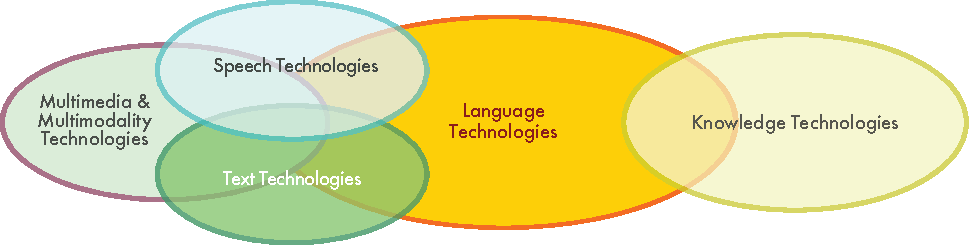
\includegraphics[width=\textwidth]{../_media/english/language_technologies}
  \caption{Language technologies}
  \label{fig:ltincontext_en}
  \colorrule{grey3}{\textwidth}{1.5pt}
\end{figure*}

When we communicate, we combine language with other modes of communication and information media -- for example speaking can involve gestures and facial expressions. Digital texts link to pictures and sounds. Movies may contain language in spoken and written form. In other words, speech and text technologies overlap and interact with other multimodal communication and multimedia technologies.\\ 
In this section, we will discuss the main application areas of language technology, i.\,e.~language checking, web search, speech interaction, and machine translation. These applications and basic technologies include: 

\begin{itemize}
\item spelling correction
\item authoring support
\item computer-assisted language learning
\item information retrieval 
\item information extraction
\item text summarisation
\item question answering
\item speech recognition 
\item speech synthesis 
\end{itemize}

Language technology is an established area of research with an
extensive set of introductory literature. The interested reader is
referred to the following references: \cite{jurafsky-martin01,
  manning-schuetze1, lt-world1, lt-survey1}.

Before discussing the above application areas, we will briefly describe the architecture of a typical LT system.

\subsection{Application Architectures}

Software applications for language processing typically consist of
several components that mirror different aspects of language. While
such applications tend to be very complex, figure~\ref{fig:textprocessingarch_en} shows a highly simplified architecture of a typical text processing system. The first three modules handle the structure and meaning of the text input:

\begin{enumerate}
\item Pre-processing: cleans the data, analyses or removes formatting, detects the input languages, and so on.
\item Grammatical analysis: finds the verb, its objects, modifiers and
  other sentence elements; detects the sentence structure.
\item Semantic analysis: performs disambiguation (i.\,e.~computes the appropriate meaning of words in a given context); resolves anaphora (i.\,e.~which pronouns refer to which nouns in the sentence); represents the meaning of the sentence in a machine-readable way.
\end{enumerate}

After analysing the text, task-specific modules can perform other operations, such as automatic summarisation and database look-ups.

In the remainder of this section, we firstly introduce the core application areas for language technology, and follow this with a brief overview of the state of LT research and education today, and a description of past and present research programmes. Finally, we present an expert estimate of core LT tools and resources for Swedish in terms of various dimensions such as availability, maturity and quality. The general situation of LT for the Swedish language is summarised in figure~\ref{fig:lrlttable_en} (p.~\pageref{fig:lrlttable_en}) at the end of this chapter. This table lists all tools and resources that are boldfaced in the text. LT support for Swedish is also compared to other languages that are part of this series.


\begin{figure*}[htb]
  \colorrule{grey3}{\textwidth}{1.5pt}
  \center
  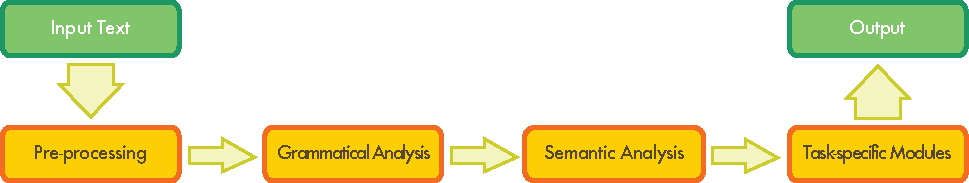
\includegraphics[width=\textwidth]{../_media/english/text_processing_app_architecture}
  \caption{A typical text processing architecture}
  \label{fig:textprocessingarch_en}
  \colorrule{grey3}{\textwidth}{1.5pt}
\end{figure*}

\subsection{Core Application Areas}

In this section, we focus on the most important LT tools and resources, and provide an overview of LT activities in Sweden. 

\subsubsection{Language Checking}

Anyone who has used a word processor such as Microsoft Word knows that
it has a spell checker that highlights spelling mistakes and proposes
corrections. The earliest spelling correction programs compared a list
of extracted words against a dictionary of correctly spelled
words. Today these programs are far more sophisticated. Using
language-dependent algorithms for \textbf{grammatical analysis}, they
detect errors related to morphology (e.\,g.~plural formation) as well
as syntax–related errors, such as a missing verb or a conflict of
verb-subject agreement (e.\,g.~\textit{she *write a
  letter}). However, most spell checkers will not find any errors in
the following text \cite{zar1}:

\begin{quote}
  I have a spelling checker,\\
  It came with my PC.\\ 
  It plane lee marks four my revue\\
  Miss steaks aye can knot sea.
\end{quote}

Handling these kinds of errors usually requires an analysis of the context. For example: 

\begin{itemize}
\item \textit{Faxen} blev tydligen \textit{skickad} förra veckan, men jag har inte sett \textit{den}.\\
=> ‘\emph{The fax} [machine] was supposedly \emph{sent} [\textsc{singular}] last week, but I have not seen \emph{it}.’
\item \textit{Faxen} blev tydligen \textit{skickade} förra veckan, men jag har inte sett \textit{dem}.\\
=> ‘\emph{The faxes} [messages] were supposedly \emph{sent} [\textsc{plural}] last week, but I have not seen \emph{them}.’
\end{itemize}

This type of analysis either needs to draw on language-specific
\textbf{grammars} laboriously coded into the software by experts, or
on a statistical language model. In this case, a model calculates the
probability of a particular word as it occurs in a specific position
(e.\,g.~between the words that precede and follow it). For example:
\textit{sölig bardisk} `soiled bar' (literally `soiled bar counter')
is a much more probable word sequence than \textit{sölig bar disk}
`soiled naked counter' (with the parts of the compound written
separately). A statistical language model can be automatically created
by using a large amount of (correct) language data, a \textbf{text
  corpus}. Most of these two approaches have been developed around
data from English. However, they do not necessarily transfer
straightforwardly to Swedish with its more flexible word order and
compound word building.

\begin{figure*}[htb]
  \colorrule{grey3}{\textwidth}{1.5pt}
  \center
  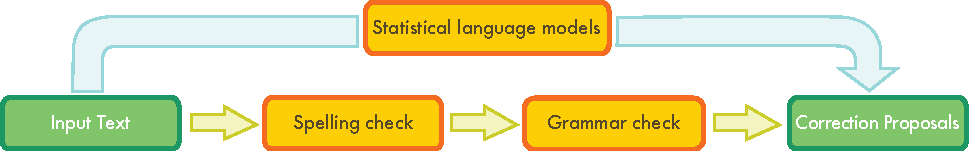
\includegraphics[width=\textwidth]{../_media/english/language_checking}
  \caption{Language checking (top: statistical; bottom: rule-based)}
  \label{fig:langcheckingaarch_en}
  \colorrule{grey3}{\textwidth}{1.5pt}
\end{figure*}

Language checking is not limited to word processors; it is also used in “authoring support systems”, i.\,e.~software environments in which manuals and other types of technical documentation for complex IT, healthcare, engineering and other products, are written. To offset customer complaints about incorrect use and damage claims resulting from poorly understood instructions, companies are increasingly focusing on the quality of technical documentation while targeting the international market (via translation or localisation) at the same time. Advances in natural language processing have led to the development of authoring support software, which helps the writer of technical documentation to use vocabulary and sentence structures that are consistent with industry rules and (corporate) terminology restrictions.

\boxtext{The use of language checking is not limited to word processors. It also applies to authoring support systems.}

Only a few Swedish companies and Language Service Providers offer products in this area, e.\,g.~Scania and some SMEs.

Besides spell checkers and authoring support, language checking is also important in the field of computer-assisted language learning. Language checking applications also automatically correct search engine queries, as found in Google's \textit{Did you mean…} suggestions.

Oribi (\url{http://www.oribi.se}) is a Swedish SME which develops
assistive technology -- including spell checking and word prediction
-- for individuals with reading and writing difficulties.

\subsubsection{Web Search}

Searching the web, intranets or digital libraries is probably the most widely used yet largely underdeveloped language technology application today. The Google search engine, which started in 1998, now handles about 80\% of all search queries \cite{spi1}. The verb \textit{googla} `to google' even has an entry in the Swedish modern dictionaries. The Google search interface and results page display has not significantly changed since the first version. However, in the current version, Google offers spelling correction for misspelled words and incorporates basic semantic search capabilities that can improve search accuracy by analysing the meaning of terms in a search query context \cite{pc1}. The Google success story shows that a large volume of data and efficient indexing techniques can deliver satisfactory results using a statistical approach to language processing. 

\boxtext{The next generation of search engines will have to include much more sophisticated\\ language technology.}

For more sophisticated information requests, it is essential to
integrate deeper linguistic knowledge to facilitate text
interpretation. Experiments using \textbf{lexical resources} such as
machine-readable thesauri or ontological language resources (e.\,g.,
WordNet for English or the Swedish
SALDO\cite{saldo1}) have
demonstrated improvements in finding pages using synonyms of the
original search terms, such as \textit{atomkraft} `atomic energy',
\textit{kärnkraft} `nuclear power' and \textit{kärnenergi} `nuclear
energy', or even more loosely related terms (such as \textit{fission}
`fission' or \textit{reaktor} `reactor').

The next generation of search engines will have to include much more
sophisticated language technology, especially to deal with search
queries consisting of a question or other sentence type rather than a
list of keywords. For the query, \textit{Give me a list of all
  companies that were taken over by other companies in the last five
  years}, a syntactic as well as \textbf{semantic analysis} is
required. The system also needs to provide an index to quickly
retrieve relevant documents. A satisfactory answer will require
syntactic parsing to analyse the grammatical structure of the sentence
and determine that the user wants companies that have been acquired,
rather than companies that have acquired other companies. For the
expression \textit{last five years}, the system needs to determine the
relevant range of years, taking into account the present year. The
query then needs to be matched against a huge amount of unstructured
data to find the pieces of information that are relevant to the user’s
request. This process is called information retrieval, and involves
searching and ranking relevant documents. To generate a list of
companies, the system also needs to recognise a particular string of
words in a document represents a company name, using a process called
named entity recognition.


\begin{figure*}[htb]
  \colorrule{grey3}{\textwidth}{1.5pt}
  \center
  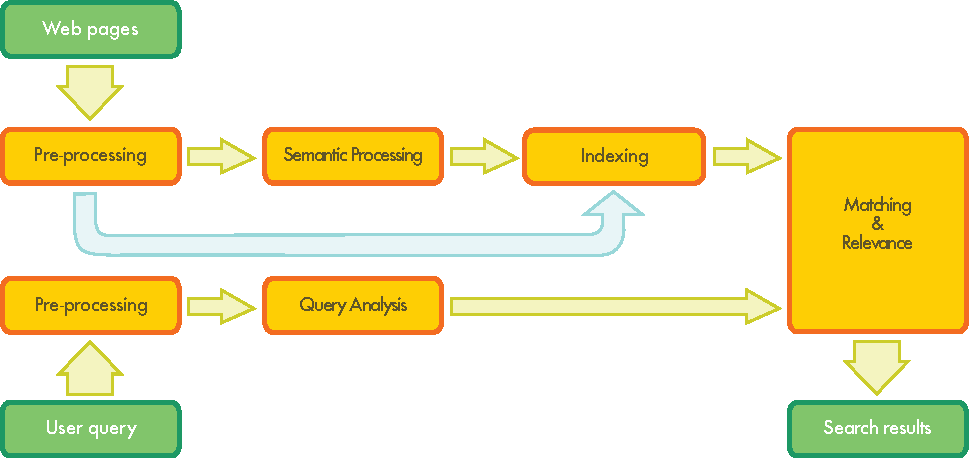
\includegraphics[width=\textwidth]{../_media/english/web_search_architecture}
  \caption{Web search}
  \label{fig:websearcharch_en}
  \colorrule{grey3}{\textwidth}{1.5pt}
 \end{figure*}

A more demanding challenge is matching a query in one language with
documents in another language. Cross-lingual information retrieval
involves automatically translating the query into all languages
present in the document collection and then translating the results
back into the user's target language.

Now that data is increasingly found in non-textual formats, there is a need for services that deliver multimedia information retrieval by searching images, audio files and video data. In the case of audio and video files, a speech recognition module must convert the speech content into text (or into a phonetic representation) that can then be matched against a user query.

Open source based technologies like Lucene and SOLr are often used by search-focused companies to provide the basic search infrastructure. Other search-based companies rely on international search technologies like, e.\,g.~FAST or Exalead.

Focus on development for companies lies on providing add-ons and advanced search engines for special-interest portals by exploiting topic-relevant semantics. Due to the still high demands in processing power, such search engines are only economically usable on relatively small text corpora. Processing time easily exceeds that of a common statistical search engine, such as e.\,g.~provided by Google, by a several orders of magnitude. These search engines also have high demand in topic-specific domain modelling, making it not feasible to use these mechanisms on web scale. 

In Sweden, Hapax (\url{http://www.hapax.com}; now Open\-Amplify) has
spent a great amount of resources on developing these technologies
around 2000–2005. Findwise (\url{http://www.findewise.com}) is a
Swedish company offering multilingual LT-enabled search solutions
primarily aimed at corporate intranets. A relatively recent Swedish
startup company is Gavagai (\url{http://www.gavagai.se}).

\subsubsection{Speech Interaction}

Speech interaction is one of many application areas that depend on speech technology, i.\,e.~technologies for processing spoken language. Speech interaction technology is used to create interfaces that enable users to interact in spoken language instead of using a graphical display, keyboard and mouse.  Today, these voice user interfaces (VUI) are used for partially or fully automated telephone services provided by companies to customers, employees or partners. Business domains that rely heavily on VUIs include banking, supply chain, public transportation, and telecommunications. Other uses of speech interaction technology include interfaces to car navigation systems and the use of spoken language as an alternative to the graphical or touchscreen interfaces in smartphones.

\begin{figure*}[htb]
  \colorrule{grey3}{\textwidth}{1.5pt}
  \center
  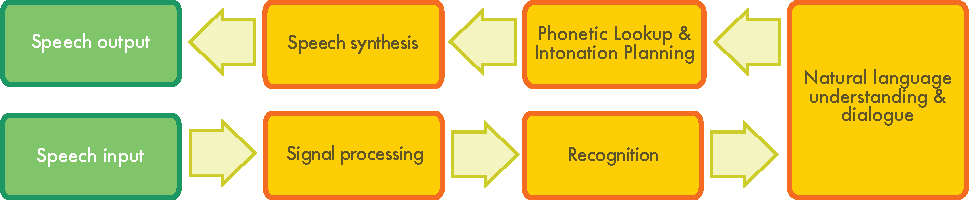
\includegraphics[width=\textwidth]{../_media/english/simple_speech-based_dialogue_architecture}
  \caption{Speech-based dialogue system}
  \label{fig:dialoguearch_en}
  \colorrule{grey3}{\textwidth}{1.5pt}
\end{figure*}

Speech interaction technology comprises four technologies: 

\begin{enumerate}
\item Automatic \textbf{speech recognition} (ASR) determines which words are actually spoken in a given sequence of sounds uttered by a user.  
\item Natural language understanding analyses the syntactic structure of a user’s utterance and interprets it according to the system in question.
\item Dialogue management determines which action to take given the user input and system functionality.   
\item \textbf{Speech synthesis} (text-to-speech or TTS) transforms the system’s reply into sounds for the user.
\end{enumerate}

One of the major challenges of ASR systems is to accurately recognise the words a user utters. This means restricting the range of possible user utterances to a limited set of keywords, or manually creating language models that cover a large range of natural language utterances. Using machine learning techniques, language models can also be generated automatically from \textbf{speech corpora}, i.\,e.~large collections of speech audio files and text transcriptions. Restricting utterances usually forces people to use the voice user interface in a rigid way and can damage user acceptance; but the creation, tuning and maintenance of rich language models will significantly increase costs. VUIs that employ language models (normally automatically created from speech corpora) and initially allow a user to express their intent more flexibly -- prompted by a \textit{How may I help you?} greeting -- are better accepted by users.

Companies tend to use utterances pre-recorded by professional speakers
for generating the output of the voice user interface. For static
utterances where the wording does not depend on particular contexts of
use or personal user data, this can deliver a rich user
experience. But more dynamic content in an utterance may suffer from
unnatural intonation because different parts of audio files have simply been strung together. Through optimisation, today’s TTS systems are getting better at producing natural-sounding dynamic utterances.

\boxtext{Speech interaction is the basis for interfaces that allow a
  user to interact with spoken language.}

Interfaces in speech interaction have been considerably standardised during the last decade in terms of their various technological components. There has also been strong market consolidation in speech recognition and speech synthesis. The national markets in the G20 countries (economically resilient countries with high populations) have been dominated by just five global players, with Nuance (USA) and Loquendo (Italy) being the most prominent players in Europe. In 2011, Nuance announced the acquisition of Loquendo, which represents a further step in market consolidation.

On the Swedish TTS market, there are voices developed e.\,g.~by Acapela, headquartered in Stockholm and also by the Swedish Library of Talking Books and Braille (TPB). There is also a strong research community mainly based at KTH, Stockholm (who have also developed their own systems).

Regarding dialogue management technology and know-how, markets are
strongly dominated by national players, which are usually
SMEs. Today’s key players in Sweden are Artificial Solutions and
SpeechCraft, and among smaller SMEs we can mention
Talkamatic (\url{http://www.talkamatic.se/}), a developer of
in-vehicle dialogue systems for the automotive industry. Rather than
exclusively relying on a product business based on software licenses,
these companies have positioned themselves mostly as full-service
providers that offer the creation of VUIs as a system integration
service. 

Finally, within the domain of speech interaction, a genuine
market for the linguistic core technologies for syntactic and semantic
analysis does not exist yet.

As for the actual employment of VUIs, demand in Sweden has strongly
increased within the last 10 years. This tendency has been driven by
end customers’ increasing demand for customer self-service and the
considerable cost optimisation aspect of automated telephone services,
as well as by a significantly increased acceptance of spoken language
as a modality for human-machine interaction. 

These factors were
catalysed by the creation of the Graduate School of Language
Technology (GSLT) network, bringing together industry players,
research institutes and enterprise customers. In collaboration with
others, the school has organised national workshops and invited
industry to give talks to the graduate students. As academic partners,
the Centre for Language Technology (CLT) at the University of
Gothenburg and the department of Speech, Music and Hearing at KTH,
Stockholm, were strongly participating in this process of spreading
the knowledge about the advantages of Speech Interaction among Swedish
enterprises. Looking ahead, there will be significant changes, due to the spread of
smartphones as a new platform for managing customer relationships, in
addition to fixed telephones, the internet and e-mail. This will also
affect how speech interaction technology is used. In the long term,
there will be more telephone-based VUIs, and spoken language apps will
play a far more central role as a user-friendly input for
smartphones. This will be largely driven by stepwise improvements in
the accuracy of speaker-independent speech recognition via the speech
dictation services already offered as centralised services to
smartphone users.

\subsubsection{Machine Translation}

\begin{figure*}[htb]
  \colorrule{grey3}{\textwidth}{1.5pt}
  \center
  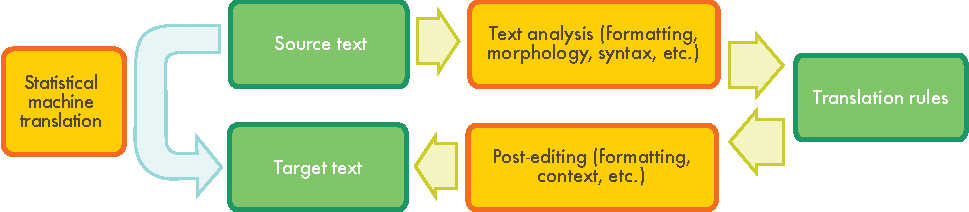
\includegraphics[width=\textwidth]{../_media/english/machine_translation}
  \caption{Machine translation (left: statistical; right: rule-based)}
  \label{fig:mtarch_en}
  \colorrule{grey3}{\textwidth}{1.5pt}
\end{figure*}


The idea of using digital computers to translate natural languages
goes back to 1946 and was followed by substantial funding for research
during the 1950s and again in the 1980s. Yet \textbf{machine
  translation} (MT) still cannot deliver on its initial promise of across-the-board automated translation. 

\boxtext{At its basic level, machine translation simply substitutes words in one natural language with words in another language.}

The most basic approach to machine translation is the automatic replacement of the words in a text written in one natural language with the equivalent words of another language. This can be useful in subject domains that have a very restricted, formulaic language such as weather reports. However, in order to produce a good translation of less restricted texts, larger text units (phrases, sentences, or even whole passages) need to be matched to their closest counterparts in the target language. The major difficulty is that human language is ambiguous. Ambiguity creates challenges on multiple levels, such as word sense disambiguation at the lexical level (a \textit{jaguar} is a brand of car or an animal) or the assignment of case on the syntactic level, for example:

\begin{itemize}
\item \textit{Polisen betraktade mannen med kikaren.}
\\`The policeman observed the man with the binoculars.'
\item \textit{Polisen betraktade mannen med revolvern.}
\\`The policeman observed the man with the revolver.'
\end{itemize}

One way to build an MT system is to use linguistic rules. For translations between closely related languages, a translation using direct substitution may be feasible, such as the one indicated above. However, rule-based (or linguistic knowledge-driven) systems often analyse the input text and create an intermediary symbolic representation from which the target language text can be generated. The success of these methods is highly dependent on the availability of extensive lexicons with morphological, syntactic, and semantic information, and large sets of grammar rules carefully designed by skilled linguists. This is a very long and therefore costly process.

In the late 1980s when computational power increased and became cheaper, interest in statistical models for machine translation began to grow. Statistical models are derived from analysing bilingual text corpora, \textbf{parallel corpora}, such as the Europarl parallel corpus, which contains the proceedings of the European Parliament in 21 European languages. Given enough data, statistical MT works well enough to derive an approximate meaning of a foreign language text by processing parallel versions and finding plausible patterns of words. Unlike knowledge-driven systems, however, statistical (or data-driven) MT systems often generate ungrammatical output. Data-driven MT is advantageous because less human effort is required, and it can also cover special particularities of the language (e.\,g.~idiomatic expressions) that are often ignored in knowledge-driven systems. 

The strengths and weaknesses of knowledge-driven and data-driven machine translation tend to be complementary, so that nowadays researchers focus on hybrid approaches that combine both methodologies. One such approach uses both knowledge-driven and data-driven systems, together with a selection module that decides on the best output for each sentence. However, results for sentences longer than, say, 12 words, will often be far from perfect. A more effective solution is to combine the best parts of each sentence from multiple outputs; this can be fairly complex, as corresponding parts of multiple alternatives are not always obvious and need to be aligned. 

\boxtext{Swedish offers several challenges for machine translation.} 

For Swedish, a challenging aspect of machine translation stems from
the possibility of creating arbitrary new words by compounding, which
makes dictionary analysis and dictionary coverage difficult. Other
challenges arise from grammatical phenomena such as word order
variation, which makes it harder to find the main functional
constituents of sentences. The alternation in particle (phrasal)
verbs between a freestanding particle in some forms and a bound prefix
in others complicates dictionary analysis.

A few machine translation systems handle Swedish currently and only a few of the larger commercial actors work on developing Swedish. In addition, there are some SMEs active in the field, e.\,g.~Convertus AB (\url{http://www.convertus.se/home-en.html}).

Provided that good adaptation is available in terms of user-specific
terminology and workflow integration, the use of machine translation
can increase productivity significantly. Commercial actors have
developed special systems for interactive translation
support. Language portals provide access to dictionaries and
company-specific terminology, translation memory and machine
translation support. An SME specializing in multilingual terminology
mining and terminology management is Fodina
Language Technology (\url{http://www.fodina.se/en}).

There is still a huge potential for improving the quality of MT systems. The challenges involve adapting language resources to a given subject domain or user area, and integrating the technology into workflows that already have term bases and translation memories. Another problem is that most of the current systems are English-centred and only support a few languages from and into Swedish. This leads to friction in the translation workflow and forces MT users to learn different lexicon coding tools for different systems.

Evaluation campaigns help to compare the quality of MT systems, the
different approaches and the status of the systems for different
language pairs. Figure~\ref{fig:euromatrix_sv}, (p.~\pageref{fig:euromatrix_sv})
which was prepared during the EC
EuroMatrix+ project, shows the pair-wise performances obtained for
22 of the 23 official EU languages (Irish was not compared). The
results are ranked according to a BLEU score, which indicates higher
scores for better translations \cite{bleu1}. A human translator would
normally achieve a score of around 80 points.

The best results (in green and blue) were achieved by languages that
benefit from a considerable research effort in coordinated programmes
and the existence of many parallel corpora (e.\,g.~English, French,
Dutch, Spanish and German). The languages with poorer results are
shown in red. These languages either lack such development efforts or
are structurally very different from the other languages (e.\,g.,
Hungarian, Maltese and Finnish).

\subsection{Other Application Areas}

Building language technology applications involves a range of subtasks that do not always surface at the level of interaction with the user, but they provide significant service functionalities “behind the scenes” of the system in question. They all form important research issues that have now evolved into individual sub-disciplines of computational linguistics.  Question answering, for example, is an active area of research for which annotated corpora have been built and scientific competitions have been initiated. The concept of question answering goes beyond keyword-based searches (in which the search engine responds by delivering a collection of potentially relevant documents) and enables users to ask a concrete question to which the system provides a single answer. For example:

\begin{itemize}
\item[] \textit{Question: How old was Neil Armstrong when he stepped on the moon?}
\item[] \textit{Answer: 38.}
\end{itemize}

While question answering is obviously related to the core area of web
search, it is nowadays an umbrella term for such research issues as which different types of questions exist, and how they should be handled; how a set of documents that potentially contain the answer can be analysed and compared (do they provide conflicting answers?); and how specific information (the answer) can be reliably extracted from a document without ignoring the context. 

\boxtext{Language technology applications often provide significant service functionalities "behind the scenes” of larger software systems.}

Question answering is in turn related to information extraction (IE),
an extremely popular and influential area when computational
linguistics took a statistical turn in the early 1990s. IE aims to
identify specific pieces of information in specific document classes, such as the key players in company takeovers as reported in newspaper stories. Another common scenario that has been studied is reports on terrorist incidents. The task here consists of mapping appropriate parts of the text to a template that specifies the perpetrator, target, time, location and results of the incident. Domain-specific template-filling is the central characteristic of IE, which makes it another example of a “behind the scenes” technology that forms a well-demarcated research area, which in practice needs to be embedded into a suitable application environment. 

Text summarisation and \textbf{text generation} are two borderline areas that can act either as standalone applications or play a supporting role. Summarisation attempts to give the essentials of a long text in a short form, and is one of the features available in Microsoft Word. It mostly uses a statistical approach to identify the “important” words in a text (i.\,e.~words that occur very frequently in the text in question but less frequently in general language use) and determine which sentences contain the most of these “important” words. These sentences are then extracted and put together to create the summary. In this very common commercial scenario, summarisation is simply a form of sentence extraction, and the text is reduced to a subset of its sentences. 

\boxtext{For Swedish, research in most text technologies is much less
  developed than for English.}

An alternative approach, for which some research has been carried out, is to generate brand new sentences that do not exist in the source text. 
This requires a deeper understanding of the text, which means that so far this approach is far less robust. On the whole, a text generator is rarely used as a stand-alone application but is embedded into a larger software environment, such as a clinical information system that collects, stores and processes patient data. Creating reports is just one of many applications for text summarisation. 

For Swedish, research in these text technologies is much less developed than for the English language. Question answering, information extraction, and summarisation have been the focus of numerous open competitions in the USA since the 1990s, primarily organised by the government-sponsored organisations DARPA (Defense Advanced Research Projects Agency) and NIST (National Institute of Standards and Technology). These competitions have significantly improved the state of the art, but their focus has mostly been on the English language; some competitions have added multilingual tracks, but Swedish was never prominent. Accordingly, there are hardly any annotated corpora or other resources for these tasks. When summarisation systems use purely statistical methods, they are largely language-independent and a number of research prototypes are available. For text generation, reusable components have traditionally been limited to surface realisation modules (generation grammars) and most of the available software is for the English language.

\subsection{Educational Programmes}

Language technology is a very interdisciplinary field that involves
the combined expertise of linguists, computer scientists,
mathematicians, philosophers, psycholinguists, and neuroscientists
among others. 

Research in language technology started in Sweden
already in the late 1960s, and after a slow but steady progress
through the 1970s and 1980s, quite a lot of resources were invested in
language technology research in the 1990s. The investments have
contributed to a relatively well-developed Swedish research community
with good organisation. In 2001, the National Graduate School of
Language Technology (GSLT) was established by the Swedish government
as one of sixteen national graduate schools. 

The graduate school is
hosted by the University of Gothenburg, but is a collaboration between
the following centres:

\begin{itemize}
\item University of Gothenburg
\item University College of Borås
\item Chalmers University of Technology (Gothenburg)
\item KTH (Royal Institute of Technology; Stockholm)
\item Linköping University
\item Lund University
\item Stockholm University
\item Uppsala University
\end{itemize}

Supervision is also available from SICS (Swedish Institute of Computer
Science; Stockholm; \url{http://www.sics.se/}). Between 2001 and
2010 the University College of Skövde and Linnaeus University (Växjö
University) were part of GSLT. At the time of writing, more than 30
PhD degrees have been awarded in the framework of GSLT, in a number of
academic subjects, but with a concentration in Linguistics, Computer
Science, and Speech Processing. GSLT has contributed significantly to
the development of language technology in Sweden bringing different
research centers and researchers together. It has made it possible to
hold national courses and provide high-quality supervision. The PhD
courses have also been offered to Nordic and Baltic PhD students
through the NGSLT (Nordic Graduate School of Language Technology)
network, funded by NorFA in the years 2004–2009. Through its national
networking aspect GSLT has also contributed to several new research
collaborations and joint proposals to national research funding
agencies.

Currently, there are two master’s programmes in language technology,
one in Gothenburg and one at Uppsala University. Up until recently
several universities also had undergraduate programmes in
computational linguistics (for example Lund University, University of
Gothenburg, Uppsala University, Stockholm University) but the number
of students has been dropping for several years, which is why new
initiatives have been taken with the master's programmes, thus
broadening the recruitment base.

\subsection{National Projects and Initiatives}

The existence of a relatively lively LT sector in Sweden can be traced
back to an early start and some major national LT programmes organised
in the last decades.

For some years the Swedish Language council and GSLT have cooperated
in building and maintaining språkteknologi.se
(\url{http://sprakteknologi.se/}), a web portal for Swedish language
technology with information about activities, resources, products and
actors, both academic and commercial. At this site, more detailed
information about these activities can be found than space permits us
to provide here.

As a result of the relatively long history of the field in Sweden,
there is an unusually large number of active language technology
research centres considering the size of the country: 

\begin{itemize}
\item Gothenburg: \emph{Centre for Language Technology}, a collaboration between University of Gothenburg and Chalmers University of Technology
\item Linköping University
\item Lund University
\item Stockholm: \emph{Center for Speech Technology} (KTH; Royal
  Institute of Technology); Stockholm University; SICS (Swedish
  Institute of Computer Science); Swedish Language Council
\item Uppsala University
\end{itemize}

As already mentioned, there is also a number of SMEs -- often
spin-offs from the academic research centers -- speech technology
being somewhat better represented than text technology, no doubt
because of the world leading research in speech technology which has
been conducted at KTH since the 1950s.

The Swedish research groups have, on the whole, worked without any
form of national coordination. However, the LT research programmes
funded in the 1990s and the existence of GSLT during the subsequent
decade have stimulated cooperation among the groups, and we have seen
research collaboration on, e.g.~\emph{machine translation and
  multilingual terminology extraction} (Gothenburg, Linköping and
Uppsala) and \emph{resource construction} (SUC -- Stockholm Umeå
Corpus).

Starting in the 1970s, Språkbanken (the Swedish Language Bank;
Gothenburg) has systematically collected, refined and distributed
Swedish language resources -- in particular rich lexical resources --
and in this connection developed tools and infrastructur for using the
resources. A current central effort is the work on the Swedish
FrameNet \cite{swefn}, a large-scale semantic lexicon resource for
Swedish.

The Center for Speech Technology at KTH (Royal Institute of
Technology; Stockholm) -- one of the leading European research centers
in the area of speech technology -- has for many years systematically
built a resource and tool base for Swedish speech technology.

During recent years, projects for automatical grammatical analysis of
Swedish have been conducted at Gothenburg, Lund and Uppsala, and
various aspects of automatic semantic processing have been developed
by these and other groups, e.g.~in the context of information access
at SICS.

Recently, Swedish research groups have joined their efforts in
national initiatives, with the primary aim of strengthening the basic
research infrastructure. These activities have resulted in some major
national proposals to the Swedish Research Council involving all the
research groups and also some other stakeholders, so far without
success, however. The need for a national LT infrastructure has now
been perceived also outside the LT research community, and the Swedish
Ministry of Culture has commissioned a report on a national linguistic
infrastructure \cite{infrarapport}.

As we have seen, previous programmes have led to the development of a
number of LT tools and resources for the Swedish language. The
following section summarises the current state of LT support for
Swedish.
  
\subsection{Availability of Tools and Resources}
\label{section:LTavailability_en}

Figure~\ref{fig:lrlttable_en} provides a rating for language technology support for the Swedish language. This rating of existing tools and resources was generated by leading experts in the field who provided estimates based on a scale from 0 (very low) to 6 (very high) using seven criteria.

\begin{figure*}[htb]
\centering
\begin{tabular}{>{\columncolor{orange1}}p{.33\linewidth}@{\hspace*{6mm}}c@{\hspace*{6mm}}c@{\hspace*{6mm}}c@{\hspace*{6mm}}c@{\hspace*{6mm}}c@{\hspace*{6mm}}c@{\hspace*{6mm}}c}
\rowcolor{orange1}
 \cellcolor{white}&
 \begin{sideways}\makecell[l]{Quantity}\end{sideways} &
 \begin{sideways}\makecell[l]{\makecell[l]{Availability} }\end{sideways} &
 \begin{sideways}\makecell[l]{Quality}\end{sideways} &
 \begin{sideways}\makecell[l]{Coverage}\end{sideways} &
 \begin{sideways}\makecell[l]{Maturity}\end{sideways} &
 \begin{sideways}\makecell[l]{Sustainability~~~}\end{sideways} &
 \begin{sideways}\makecell[l]{Adaptability}\end{sideways} \\ \addlinespace
\multicolumn{8}{>{\columncolor{orange2}}l}{Language Technology: Tools, Technologies and Applications} \\ \addlinespace
Speech Recognition &2&1&3&4&5&5&5 \\ \addlinespace
Speech Synthesis &3&1&3&3&3&3&3 \\ \addlinespace 
Grammatical analysis &4.5&3.5&5&4&5&5&5 \\ \addlinespace 
Semantic analysis &1.5&1&2&1.5&1.5&1&1.5 \\ \addlinespace
Text generation &3&3&3&2&4&3&4 \\ \addlinespace 
Machine translation &3&1&3&1&4&3&3 \\ \addlinespace 
\multicolumn{8}{>{\columncolor{orange2}}l}{Language Resources: Resources, Data and Knowledge Bases} \\ \addlinespace
Text corpora &2&2.5&3.5&3&5&5&5 \\ \addlinespace 
Speech corpora &4&3&3&3&5&4&4 \\ \addlinespace 
Parallel corpora &3&1&5&3&5&5&5 \\ \addlinespace 
Lexical resources &4&2&5&4&3.5&4&4 \\ \addlinespace 
Grammars &3&2&3&3&3&4&5 \\ 
\end{tabular}
\caption{State of language technology support for Swedish}
\label{fig:lrlttable_en}
\end{figure*}

The key results for Swedish language technology can be summed up as follows:

\begin{itemize}
\item On the one hand, processing of written text currently seems to
  be more mature than speech processing. On the other hand, speech
  technology -- and less so text technology -- has already been
  successfully integrated into many everyday applications, from spoken
  dialogue systems and voice-based interfaces to mobile phones and car
  navigation systems.
\item As for many other languages, it is clear that the ``lower''
  levels of linguistic analysis -- e.\,g.~morphological and syntactic
  processing, as well as basic speech processing -- are much better
  catered for than, e.\,g.~semantics, text linguistics and
  pragmatics. Advanced technologies that require deep linguistic
  processing and semantic knowledge are still in their infancy.
\item As to resources, if we think of the Swedish situation in terms
  of the BLARK (Basic LAnguage Resource Kit) concept \cite{blark,sweblark}, we
  may note that there is a conspicuous lack of certain basic
  resources:
%\begin{itemize}

While there are some -- mainly small -- specific corpora of high
quality, a large balanced corpus (a ``national corpus'') \cite{SNK}
does not exist, nor is a large syntactically annotated and manually
validated corpus (treebank) available for Swedish. Corpus access is
also generally restricted because many copyright issues remain to be
resolved.

No full-scale Swedish wordnet is available to the language
  technology community.

In the area of multilingual resources, there is a clear focus on
  Swedish--English resources (and Swedish--English/English--Swedish
  machine translation), and not much in the way of support for other
  languages, e.\,g.~the national minority languages, other Nordic
  languages, and other important European and world languages than
  English.
%\end{itemize}
\item Many of the tools and resources lack standardisation, i.\,e.~even
  if they exist, sustainability and interoperability are not a given;
  concerted programmes and initiatives are needed to standardise data,
  information models and interchange formats.
\item An unclear legal situation restricts the use of digital texts,
  e.\,g.~those published online by newspapers, for empirical
  linguistic and language technology research, such as training
  statistical language models. Together with politicians and policy
  makers, researchers should try to establish laws or regulations that
  enable researchers to use publicly available texts for
  language-related R\&D activities.
\item The cooperation between the language technology community and
  those involved with the Semantic Web and the closely related Linked
  Open Data movement should be intensified with the goal of
  establishing a collaboratively maintained, machine-readable
  knowledge base that can be used both in web-based information
  systems and as semantic knowledge bases in LT applications. Ideally,
  this endeavour should be addressed multilingually on the European
  scale.
\end{itemize}

The most urgent needs of Swedish language technology at present are
(in order of decreasing feasibility/increasing cost):
\begin{enumerate}
\item Standardisation (for interoperabilty, of data and content
  formats, as well as APIs) of existing basic open source/open content
  tools and resources, in order to make them generally available to
  the research community and industry.
\item Negotiations with the aim of improving licensing conditions of
  other existing basic tools and resources. If negotiations are
  successful, such tools and resources can then be standardised as in
  the preceding point.
\item Creation of missing basic tools and resources in standard
  formats with maximally open licenses, e.\,g.~a Swedish national
  corpus (which could include a treebank component and a number of
  parallel corpora) \cite{SNK} and a full-scale open Swedish wordnet linked to
  the English Princeton WordNet.
\item Basic research on the higher levels of automatic linguistic
  analysis for Swedish, and on integration of statistical and
  rule-based language technology, not least in order to aim for a
  closer interaction between speech and text technology.
\end{enumerate}


\subsection{Cross-language comparison}

The current state of LT support varies considerably from one language community to another. In order to compare the situation between languages, this section will present an evaluation based on two sample application areas (machine translation and speech processing) and one underlying technology (text analysis), as well as basic resources needed for building LT applications. The languages were categorised using the following five-point scale: 

\begin{enumerate}
\item Excellent support
\item Good support
\item Moderate support
\item Fragmentary support
\item Weak or no support
\end{enumerate}

LT support was measured according to the following criteria:

\textbf{Speech processing:} Quality of existing speech recognition technologies, quality of existing speech synthesis technologies, coverage of domains, number and size of existing speech corpora, amount and variety of available speech-based applications.

\textbf{Machine translation:} Quality of existing MT technologies, number of language pairs covered, coverage of linguistic phenomena and domains, quality and size of existing parallel corpora, amount and variety of available MT applications.

\textbf{Text analysis:} Quality and coverage of existing text analysis technologies (morphology, syntax, semantics), coverage of linguistic phenomena and domains, amount and variety of available applications, quality and size of existing (annotated) text corpora, quality and coverage of existing lexical resources (e.\,g.~WordNet) and grammars.

\textbf{Resources:} Quality and size of existing text corpora, speech corpora and parallel corpora, quality and coverage of existing lexical resources and grammars.

Figures~\ref{fig:speech_cluster_en} to~\ref{fig:resources_cluster_en}
show that, first of all, English is in a class of its own when it
comes to both basic application areas and language technology
resources, being in the lead in almost all LT areas. And yet there are
still plenty of gaps in English language resources with regard to high
quality applications.

Thanks to an active LT research community with roots going back to the
1960s, and thanks to the national LT funding programmes of the 1990s,
Swedish generally falls somewhere in the middle in comparison with
other European languages. It fares better in the area of language
resources, but worse when it comes to machine translation.

\boxtext{Swedish generally falls somewhere in the middle in comparison with
other European languages.}

For speech processing, current technologies perform well enough to be
successfully integrated into a number of industrial applications such
as spoken dialogue and dictation systems. Today's text analysis
components and language resources already cover the linguistic
phenomena of Swedish to a certain extent and form part of many
applications involving mostly shallow natural language processing,
e.\,g. spelling correction and authoring support.

However, for building more sophisticated applications, such as
high-quality machine translation between Swedish and several other
languages, there is a clear need for resources and technologies that
cover a wider range of linguistic aspects and enable a deep semantic
analysis of the input text. By improving the quality and coverage of
these basic resources and technologies, we shall be able to open up
new opportunities for tackling a broader range of advanced application
areas.


\subsection{Conclusions}

\emph{In this series of white papers, we have provided the first high-level comparison of language technology support across 30 European languages.
By identifying the gaps, needs and deficits, the European language technology community and its related stakeholders are now in a position to design a large scale research and development programme aimed at building truly multilingual, technology-enabled communication across Europe.}

The results of this white paper series show that there is a dramatic difference in language technology support between the various European languages. While there are good quality software and resources available for some languages and application areas, others, usually smaller languages, have substantial gaps. Many languages lack basic technologies for text analysis and the essential resources. Others have basic tools and resources but the implementation of, for example, semantic methods is still far away. Therefore a large-scale effort is needed to attain the ambitious goal of providing high-quality language technology support for all European languages, for example through high quality machine translation. 

As already mentioned, Language Technology research has been pursued in
Sweden since the 1960s, and the research community forms a close-knit
national network, in no small part due to the existence of the
national graduate school of language technology. 

Compared to many
other languages, Swedish is reasonably well endowed with language
tools and resources. However, there is certainly room for improvement;
the scope of the resources and the range of tools are still very
limited when compared to English and some other major languages, and
they are simply not sufficient in quality and quantity to develop the
kind of technologies required to support a truly multilingual
knowledge society. Also, in many cases, although tools and resources
exist, their wider use is hampered by proprietary licenses or arcane
data formats, or both. 

We cannot simply transfer technologies already developed and
optimised for the English language to handle Swedish. English-based
systems for grammatical analysis of word and sentence structure
typically perform far less well on Swedish texts, due to the specific
characteristics of the Swedish language. Our findings lead to the conclusion that the only way forward is to make a substantial effort to create language technology resources for Swedish, as a means to drive forward research, innovation and development. The need for large amounts of data and the extreme complexity of language technology systems makes it vital to develop an infrastructure and a coherent research organisation to spur greater sharing and cooperation.

Finally there is a lack of continuity in research and development funding. Short-term coordinated programmes tend to alternate with periods of sparse or zero funding. In addition, there is an overall lack of coordination with programmes in other EU countries and at the European Commission level.

The long term goal of META-NET is to enable the creation of
high-quality language technology for all languages. This requires all
stakeholders -- in politics, research, business, and society -- to
unite their efforts. The resulting technology will help tear down
existing barriers and build bridges between Europe’s languages, paving
the way for political and economic unity through cultural diversity.
\end{multicols}

\clearpage

\begin{figure*}
\small
\centering
\begin{tabular}
{ % defines color for each column.
>{\columncolor{corange5}}p{.15\linewidth}@{\hspace{.04\linewidth}}
>{\columncolor{corange4}}p{.15\linewidth}@{\hspace{.04\linewidth}}
>{\columncolor{corange3}}p{.15\linewidth}@{\hspace{.04\linewidth}}
>{\columncolor{corange2}}p{.15\linewidth}@{\hspace{.04\linewidth}}
>{\columncolor{corange1}}p{.15\linewidth} 
}
\rowcolor{white} % redefines color for all columns in row 1
\begin{center}\textbf{Excellent support}\vspace*{-2mm}\end{center} & 
\begin{center}\textbf{Good support}\vspace*{-2mm}\end{center} & 
\begin{center}\textbf{Moderate support}\vspace*{-2mm}\end{center} & 
\begin{center}\textbf{Fragmentary support}\vspace*{-2mm}\end{center} & 
\begin{center}\textbf{Weak/no support}\vspace*{-2mm}\end{center} \\

& \vspace*{0.5mm}English
& \vspace*{0.5mm}
  Czech \newline 
  Dutch \newline 
  Finnish \newline 
  French \newline 
  German \newline   
  Italian \newline  
  Portuguese \newline 
  Spanish \newline
& \vspace*{0.5mm}Basque \newline 
  Bulgarian \newline 
  Catalan \newline 
  Danish \newline 
  Estonian \newline 
  Galician\newline 
  Greek \newline  
  Hungarian  \newline
  Irish \newline  
  Norwegian \newline 
  Polish \newline 
  Serbian \newline 
  Slovak \newline 
  Slovene \newline 
  \textbf{{Swedish}} \newline
& \vspace*{0.5mm}
  Croatian \newline 
  Icelandic \newline  
  Latvian \newline 
  Lithuanian \newline 
  Maltese \newline 
  Romanian\newline
\end{tabular}
\caption{Speech processing: State of language technology support for 30 European languages}
\label{fig:speech_cluster_en}
\end{figure*}

\begin{figure*}
\small
\centering
\begin{tabular}
{ % defines color for each column.
>{\columncolor{corange5}}p{.15\linewidth}@{\hspace{.04\linewidth}}
>{\columncolor{corange4}}p{.15\linewidth}@{\hspace{.04\linewidth}}
>{\columncolor{corange3}}p{.15\linewidth}@{\hspace{.04\linewidth}}
>{\columncolor{corange2}}p{.15\linewidth}@{\hspace{.04\linewidth}}
>{\columncolor{corange1}}p{.15\linewidth} 
}
\rowcolor{white} % redefines color for all columns in row 1
\begin{center}\textbf{Excellent support}\vspace*{-2mm}\end{center} & 
\begin{center}\textbf{Good support}\vspace*{-2mm}\end{center} & 
\begin{center}\textbf{Moderate support}\vspace*{-2mm}\end{center} & 
\begin{center}\textbf{Fragmentary support}\vspace*{-2mm}\end{center} & 
\begin{center}\textbf{Weak/no support}\vspace*{-2mm}\end{center} \\ 

& \vspace*{0.5mm} English 
& \vspace*{0.5mm} 
  French \newline 
  Spanish
& \vspace*{0.5mm}
  Catalan \newline 
  Dutch \newline 
  German \newline 
  Hungarian \newline
  Italian \newline 
  Polish \newline 
  Romanian \newline 
& \vspace*{0.5mm}Basque \newline 
  Bulgarian \newline 
  Croatian \newline 
  Czech \newline
  Danish \newline 
  Estonian \newline 
  Finnish \newline 
  Galician \newline 
  Greek \newline 
  Icelandic \newline 
  Irish \newline 
  Latvian \newline 
  Lithuanian \newline 
  Maltese \newline 
  Norwegian \newline 
  Portuguese \newline 
  Serbian \newline 
  Slovak \newline 
  Slovene \newline 
  \textbf{Swedish}\newline 
\end{tabular}
\caption{Machine translation: State of language technology support for 30 European languages}
\label{fig:mt_cluster_en}
\end{figure*}

\begin{figure*}
\small
\centering
\begin{tabular}
{ % defines color for each column.
>{\columncolor{corange5}}p{.15\linewidth}@{\hspace{.04\linewidth}}
>{\columncolor{corange4}}p{.15\linewidth}@{\hspace{.04\linewidth}}
>{\columncolor{corange3}}p{.15\linewidth}@{\hspace{.04\linewidth}}
>{\columncolor{corange2}}p{.15\linewidth}@{\hspace{.04\linewidth}}
>{\columncolor{corange1}}p{.15\linewidth} 
}
\rowcolor{white} % redefines color for all columns in row 1
\begin{center}\textbf{Excellent support}\vspace*{-2mm}\end{center} & 
\begin{center}\textbf{Good support}\vspace*{-2mm}\end{center} & 
\begin{center}\textbf{Moderate support}\vspace*{-2mm}\end{center} & 
\begin{center}\textbf{Fragmentary support}\vspace*{-2mm}\end{center} & 
\begin{center}\textbf{Weak/no support}\vspace*{-2mm}\end{center} \\

& \vspace*{0.5mm}English
& \vspace*{0.5mm}
  Dutch \newline 
  French \newline 
  German \newline 
  Italian \newline 
  Spanish
& \vspace*{0.5mm}Basque \newline 
  Bulgarian \newline 
  Catalan \newline 
  Czech \newline 
  Danish \newline 
  Finnish \newline 
  Galician \newline 
  Greek \newline 
  Hungarian \newline 
  Norwegian \newline 
  Polish \newline 
  Portuguese \newline 
  Romanian \newline 
  Slovak \newline 
  Slovene \newline 
  \textbf{{Swedish}} \newline 
& \vspace*{0.5mm}
  Croatian \newline 
  Estonian \newline 
  Icelandic \newline 
  Irish \newline 
  Latvian \newline 
  Lithuanian \newline 
  Maltese \newline 
  Serbian \\
  \end{tabular}
\caption{Text analysis: State of language technology support for 30 European languages}
\label{fig:text_cluster_en}
\end{figure*}

\begin{figure*}
\small
\centering
\begin{tabular}
{ % defines color for each column.
>{\columncolor{corange5}}p{.15\linewidth}@{\hspace{.04\linewidth}}
>{\columncolor{corange4}}p{.15\linewidth}@{\hspace{.04\linewidth}}
>{\columncolor{corange3}}p{.15\linewidth}@{\hspace{.04\linewidth}}
>{\columncolor{corange2}}p{.15\linewidth}@{\hspace{.04\linewidth}}
>{\columncolor{corange1}}p{.15\linewidth} 
}
\rowcolor{white} % redefines color for all columns in row 1
\begin{center}\textbf{Excellent support}\vspace*{-2mm}\end{center} & 
\begin{center}\textbf{Good support}\vspace*{-2mm}\end{center} & 
\begin{center}\textbf{Moderate support}\vspace*{-2mm}\end{center} & 
\begin{center}\textbf{Fragmentary support}\vspace*{-2mm}\end{center} & 
\begin{center}\textbf{Weak/no support}\vspace*{-2mm}\end{center} \\
    
& \vspace*{0.5mm}English
& \vspace*{0.5mm} 
    Czech \newline 
    Dutch \newline 
    French \newline 
    German \newline 
    Hungarian \newline
    Italian \newline
    Polish \newline
    Spanish \newline
    \textbf{{Swedish}} \newline 
& \vspace*{0.5mm} Basque\newline 
    Bulgarian\newline 
    Catalan \newline 
    Croatian \newline 
    Danish \newline 
    Estonian \newline 
    Finnish \newline 
    Galician \newline 
    Greek \newline 
    Norwegian \newline 
    Portuguese \newline 
    Romanian \newline 
    Serbian \newline 
    Slovak \newline 
    Slovene \newline
&  \vspace*{0.5mm}
    Icelandic \newline 
    Irish \newline 
    Latvian \newline 
    Lithuanian \newline 
    Maltese  \\
  \end{tabular}
  \caption{Speech and text resources: State of support for 30 European languages}
  \label{fig:resources_cluster_en}
\end{figure*}

\clearpage

\ssection[About META-NET]{About META-NET}

\begin{multicols}{2}
META-NET is a Network of Excellence partially funded by the European
Commission \cite{rehm2011}. The network currently consists of 54 research centres in 33 European countries. META-NET forges META, the Multilingual Europe Technology Alliance, a growing community of language technology professionals and organisations in Europe. META-NET fosters the technological foundations for a truly multilingual European information society that: 

\begin{itemize}
\item makes communication and cooperation possible across languages;
\item grants all Europeans equal access to information and knowledge regardless of their language; 
\item builds upon and advances functionalities of networked information technology.
\end{itemize}

The network supports a Europe that unites as a single digital market
and information space. It stimulates and promotes multilingual
technologies for all European languages. These technologies support
automatic translation, content production, information processing and
knowledge management for a wide variety of subject domains and
applications. They also enable intuitive language-based interfaces to
technology ranging from household electronics, machinery and vehicles
to computers and robots. Launched on 1 February 2010, META-NET has already conducted various activities in its three lines of action META-VISION, META-SHARE and META-RESEARCH. 

\textbf{META-VISION} fosters a dynamic and influential stakeholder community that unites around a shared vision and a common strategic research agenda (SRA). The main focus of this activity is to build a coherent and cohesive LT community in Europe by bringing together representatives from highly fragmented and diverse groups of stakeholders. The present White Paper was prepared together with volumes for 29 other languages. The shared technology vision was developed in three sectorial Vision Groups. The META Technology Council was established in order to discuss and to prepare the SRA based on the vision in close interaction with the entire LT community. 

\textbf{META-SHARE} creates an open, distributed facility for exchanging and sharing resources. The peer-to-peer network of repositories will contain language data, tools and web services that are documented with high-quality metadata and organised in standardised categories. The resources can be readily accessed and uniformly searched. The available resources include free, open source materials as well as restricted, commercially available, fee-based items. 

\textbf{META-RESEARCH} builds bridges to related technology
fields. This activity seeks to leverage advances in other fields and to
capitalise on innovative research that can benefit language
technology. In particular, the action line focuses on conducting
leading-edge research in machine translation, collecting data, preparing data sets and organising language resources for evaluation purposes; compiling inventories of tools and methods; and organising workshops and training events for members of the community. \\\\

\textbf{\centerline{office@meta-net.eu -- http://www.meta-net.eu}}
\end{multicols}

\cleardoublepage

\appendix
\addtocontents{toc}{\protect\bigskip}

\cleardoublepage

\phantomsection\bsection[Litteratur -- References]{Litteratur --- References}
\bibliographystyle{unsrt}
\bibliography{swedish_references}
  
\cleardoublepage

\phantomsection\bsection[Medlemmar i META-NET -- META-NET Members]{META-NETs
  medlemmar --- META-NET \ \ \ \ \ \  Members}
\label{metanetmembers}

\small
\begin{longtable}{llp{114mm}}
  Belgien & \textcolor{grey1}{Belgium} & Computational Linguistics and Psycholinguistics Research Centre, University of Antwerp: Walter Daelemans\\ \addlinespace
  & & Centre for Processing Speech and Images, University of Leuven: Dirk van Compernolle \\ \addlinespace
  Bulgarien & \textcolor{grey1}{Bulgaria} & Institute for Bulgarian Language, Bulgarian Academy of Sciences: Svetla Koeva \\ \addlinespace
  Cypern &  \textcolor{grey1}{Cyprus} & Language Centre, School of Humanities: Jack Burston\\ \addlinespace
  Danmark &  \textcolor{grey1}{Denmark} & Centre for Language Technology, University of Copenhagen: \newline Bolette Sandford Pedersen, Bente Maegaard\\ \addlinespace
  Estland & \textcolor{grey1}{Estonia} & Institute of Computer Science, University of Tartu: Tiit Roosmaa, Kadri Vider\\ \addlinespace
  Finland & \textcolor{grey1}{Finland} & Computational Cognitive Systems Research Group, Aalto University: Timo Honkela\\ \addlinespace
  & & Department of Modern Languages, University of Helsinki: Kimmo Koskenniemi,\newline Krister Lindén \\ \addlinespace
  Frankrike & \textcolor{grey1}{France} & Centre National de la Recherche Scientifique, Laboratoire d'Informatique pour la Mécanique et les Sciences de l'Ingénieur and Institute for Multilingual and Multimedia Information: Joseph Mariani \\ \addlinespace
  & & Evaluations and Language Resources Distribution Agency: Khalid Choukri\\ \addlinespace
  Grekland & \textcolor{grey1}{Greece} & R.C. “Athena”, Institute for
  Language and Speech Processing: Stelios Piperidis\\ \addlinespace
  Irland & \textcolor{grey1}{Ireland} & School of Computing, Dublin City University: Josef van Genabith\\ \addlinespace
  Island & \textcolor{grey1}{Iceland} & School of Humanities, University of Iceland: Eiríkur Rögnvaldsson\\ \addlinespace
  Italien & \textcolor{grey1}{Italy} & Consiglio Nazionale delle Ricerche, Istituto di Linguistica Computazionale “Antonio Zampolli”: Nicoletta Calzolari\\ \addlinespace
  & & Human Language Technology Research Unit, Fondazione Bruno Kessler:\newline Bernardo Magnini\\ \addlinespace 
  Kroatien & \textcolor{grey1}{Croatia} & Institute of Linguistics, Faculty of Humanities and Social Science, University of Zagreb: Marko Tadić \\ \addlinespace
  Lettland & \textcolor{grey1}{Latvia} & Tilde: Andrejs Vasiļjevs\\ \addlinespace 
  & & Institute of Mathematics and Computer Science, University of Latvia: Inguna Skadiņa\\ \addlinespace
  Litauen & \textcolor{grey1}{Lithuania} & Institute of the Lithuanian Language: Jolanta Zabarskaitė\\ \addlinespace
  Luxemburg & \textcolor{grey1}{Luxembourg} & Arax Ltd.: Vartkes Goetcherian\\ \addlinespace
  Malta & \textcolor{grey1}{Malta} & Department Intelligent Computer Systems, University of Malta: Mike Rosner\\ \addlinespace
  Nederländerna & \textcolor{grey1}{Netherlands} & Utrecht Institute of Linguistics, Utrecht University: Jan Odijk\\ \addlinespace 
  & & Computational Linguistics, University of Groningen: Gertjan van Noord\\ \addlinespace
  Norge & \textcolor{grey1}{Norway} & Department of Linguistic,
  Literary and Aesthetic Studies, University of Bergen:\newline Koenraad De Smedt\\ \addlinespace 
  & & Department of Informatics, Language Technology Group, University of Oslo:\newline Stephan Oepen \\ \addlinespace
  Österrike  & \textcolor{grey1}{Austria} & Zentrum für Translationswissenschaft, Universität Wien: Gerhard Budin\\ \addlinespace 
  Polen & \textcolor{grey1}{Poland} & Institute of Computer Science, Polish Academy of Sciences: Adam Przepiórkowski,\newline Maciej Ogrodniczuk \\ \addlinespace
  & & University of Łódź: Barbara Lewandowska-Tomaszczyk, Piotr Pęzik\\ \addlinespace
  & & Department of Computer Linguistics and Artificial Intelligence, Adam Mickiewicz University: Zygmunt Vetulani \\ \addlinespace
  Portugal & \textcolor{grey1}{Portugal} & University of Lisbon: António Branco, Amália Mendes \\ \addlinespace
  & & Spoken Language Systems Laboratory, Institute for Systems Engineering and Computers: Isabel Trancoso \\ \addlinespace
  Rumänien & \textcolor{grey1}{Romania} & Research Institute for Artificial Intelligence, Romanian Academy of Sciences: Dan Tufiș \\ \addlinespace
  & & Faculty of Computer Science, University Alexandru Ioan Cuza of
  Iași: Dan Cristea \\ \addlinespace
  Schweiz & \textcolor{grey1}{Switzerland} & Idiap Research Institute: Hervé Bourlard \\ \addlinespace 
  Serbien & \textcolor{grey1}{Serbia} & University of Belgrade, Faculty of Mathematics: Duško Vitas, Cvetana Krstev,\newline Ivan Obradović \\ \addlinespace
  & & Pupin Institute: Sanja Vranes \\ \addlinespace  
  Slovakien & \textcolor{grey1}{Slovakia} & Ľudovít Štúr Institute of Linguistics, Slovak Academy of Sciences: Radovan Garabík \\ \addlinespace 
  Slovenien & \textcolor{grey1}{Slovenia} & Jožef Stefan Institute: Marko Grobelnik \\ \addlinespace 
  Spanien & \textcolor{grey1}{Spain} & Barcelona Media: Toni Badia, Maite Melero \\ \addlinespace 
  & & Institut Universitari de Lingüística Aplicada, Universitat Pompeu Fabra: Núria Bel \\ \addlinespace 
  & & Aholab Signal Processing Laboratory, University of the Basque Country:\newline Inma Hernaez Rioja \\ \addlinespace 
  & & Centre for Language and Speech Technologies and Applications, Universitat Politècnica de Catalunya:  Asunción Moreno \\ \addlinespace 
  & & Department of Signal Processing and Communications, University
  of Vigo:\newline Carmen García Mateo \\ \addlinespace 
  Storbritannien & \textcolor{grey1}{UK} & 
  School of Computer Science, University of Manchester: Sophia Ananiadou \\ \addlinespace 
  & & Institute for Language, Cognition and Computation, Centre for Speech Technology Research, University of Edinburgh: Steve Renals \\ \addlinespace 
  & & Research Institute of Informatics and Language Processing,
  University of Wolverhampton: Ruslan Mitkov \\ \addlinespace  
  Sverige & \textcolor{grey1}{Sweden} & Språkbanken, Department of Swedish, University of Gothenburg: Lars Borin \\ \addlinespace
  Tjeckien & \textcolor{grey1}{Czech Republic} & Institute of Formal and Applied Linguistics, Charles University in Prague: Jan Hajič \\ \addlinespace
  Tyskland & \textcolor{grey1}{Germany} & Language Technology Lab, DFKI: Hans Uszkoreit, Georg Rehm\\ \addlinespace
  & & Human Language Technology and Pattern Recognition, RWTH Aachen University: Hermann Ney \\ \addlinespace
  & & Department of Computational Linguistics, Saarland University: Manfred Pinkal\\ \addlinespace   
  Ungern & \textcolor{grey1}{Hungary} & Research Institute for Linguistics, Hungarian Academy of Sciences: Tamás Váradi\\  \addlinespace
  & & Department of Telecommunications and Media Informatics, Budapest University of Technology and Economics: Géza Németh, Gábor Olaszy
\end{longtable}
\normalsize

\renewcommand*{\figureformat}{}
\renewcommand*{\captionformat}{}

\begin{figure*}[htbp]
   \colorrule{grey3}{\textwidth}{1.5pt}
  \center
  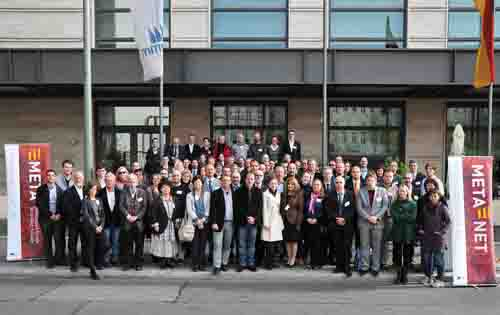
\includegraphics[width=\textwidth]{../_media/meta-net_team.jpg}
  \caption{Närmare 100 språkteknologiexperter -- från länderna och
    språkgemenskaperna i META-NET -- diskuterade och finputsade
    höjdpunkterna i vitböckerna vid ett META-NET-möte i Berlin den
    21--22 oktober 2011. --- \textcolor{grey1}{About 100 language
      technology experts -- representatives of the countries and
      languages represented in META-NET -- discussed and finalised the
      key results and messages of the White Paper Series at a META-NET
      meeting in Berlin, Germany, on October 21/22, 2011.}}
  \colorrule{grey3}{\textwidth}{1.5pt}
\end{figure*}

\cleardoublepage

\phantomsection\bsection[META-NETs vitböcker -- The META-NET White Paper
Series]{META-NETs vitböcker --- The META-NET \ \ \ \ \ \ \ \ White Papers}% Series}
\label{whitepaperseries}

\vspace*{-5mm}
\centering
  \setlength{\tabcolsep}{2.5em}
  \begin{tabularx}{\textwidth}{lllll} \toprule\addlinespace
%  \begin{tabulary}{170mm}{LLL} \toprule
  &baskiska & Basque & euskara\\
  &bulgariska & Bulgarian & български\\
  &danska & Danish & dansk\\
  &engelska & English & English\\
  &estniska & Estonian & eesti\\
  &finska & Finnish & suomi\\
  &franska & French & français\\
  &galiciska & Galician & galego\\
  &grekiska & Greek & ελληνικά\\
  &iriska & Irish & Gaeilge\\
  &isländska & Icelandic & íslenska\\
  &italienska & Italian & italiano\\
  &katalanska & Catalan & català\\
  &kroatiska & Croatian & hrvatski\\
  &lettiska & Latvian & latviešu valoda\\
  &litauiska & Lithuanian & lietuvių kalba\\
  &maltesiska & Maltese & Malti\\
  &nederländska & Dutch & Nederlands\\
  &norska bokmål & Norwegian Bokmål & bokmål\\
  &nynorska & Norwegian Nynorsk & nynorsk\\
  &polska & Polish & polski\\
  &portugisiska & Portuguese & português\\
  &rumänska & Romanian & română\\
  &serbiska & Serbian & српски\\
  &slovakiska & Slovak & slovenčina\\
  &slovenska & Slovene & slovenščina\\
  &spanska & Spanish & español\\
  &svenska & Swedish & svenska\\
  &tjeckiska & Czech & čeština\\
  &tyska & German & Deutsch\\
  &ungerska & Hungarian & magyar\\ \addlinespace \bottomrule
\end{tabularx}
